\documentclass[a4paper]{article}

\usepackage[english]{babel}
\usepackage[utf8]{inputenc}
\usepackage{amsmath}
\usepackage{graphicx}
\usepackage{enumerate}
\usepackage{caption}
\usepackage[colorinlistoftodos]{todonotes}
\usepackage{graphicx}
\usepackage{advdate}
\usepackage{listings}
\usepackage{color}%red, green, blue, yellow, cyan, magenta, black, white
\definecolor{mygreen}{RGB}{28,172,0}% color values Red, Green, Blue
\definecolor{mylilas}{RGB}{170,55,241}
\graphicspath{c:/Users/Max/Pictures}
\title{AE 370: Finite Element Project}
\lstset{language=Matlab,%
    %basicstyle=\color{red},
    breaklines=true,%
    morekeywords={matlab2tikz},
    keywordstyle=\color{blue},%
    morekeywords=[2]{1}, keywordstyle=[2]{\color{black}},
    identifierstyle=\color{black},%
    stringstyle=\color{mylilas},
    commentstyle=\color{mygreen},%
    showstringspaces=false,%without this there will be a symbol in the places where there is a space
    numbers=left,%
    numberstyle={\tiny \color{black}},% size of the numbers
    numbersep=9pt, % this defines how far the numbers are from the text
    emph=[1]{for,end,break},emphstyle=[1]\color{red}, %some words to emphasise
    %emph=[2]{word1,word2}, emphstyle=[2]{style},    
}
\author{Max A. Feinberg, Mike O'Connell}

\date{\AdvanceDate[-1]\today}

\begin{document}
\maketitle

Utilizing the finite element analysis (FEA) software package, Abaqus, the following cantilever linearly elastic beam problem was analyzed:

\begin{figure}[ht]
\centering
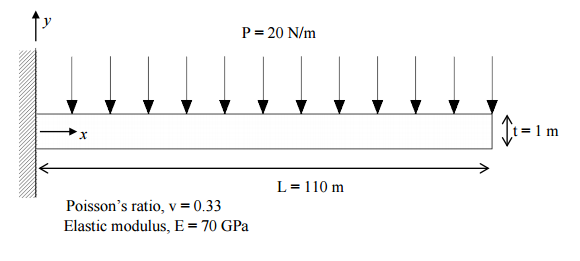
\includegraphics[scale=.75]{beam.PNG}
\caption{A linearly Elastic Cantilever Beam Subjected to Uniform Pressure}
\end{figure}
\textbf{a)}\\

The problem was initially analyzed using 3-node plane stress triangular elements.  The stress and deflection contours for the simulations can be found on the following pages in Figure 2 through Figure 21.  The first contour plot on each page is a stress contour and the second contour plot is a deflection contour.  The element size, the number of nodes, and the number of elements used in each simulation can be found in the caption under each figure. The maximum deflection magnitude can also be found in the caption of each deflection contour plot.

\begin{figure}[ht]
\centering
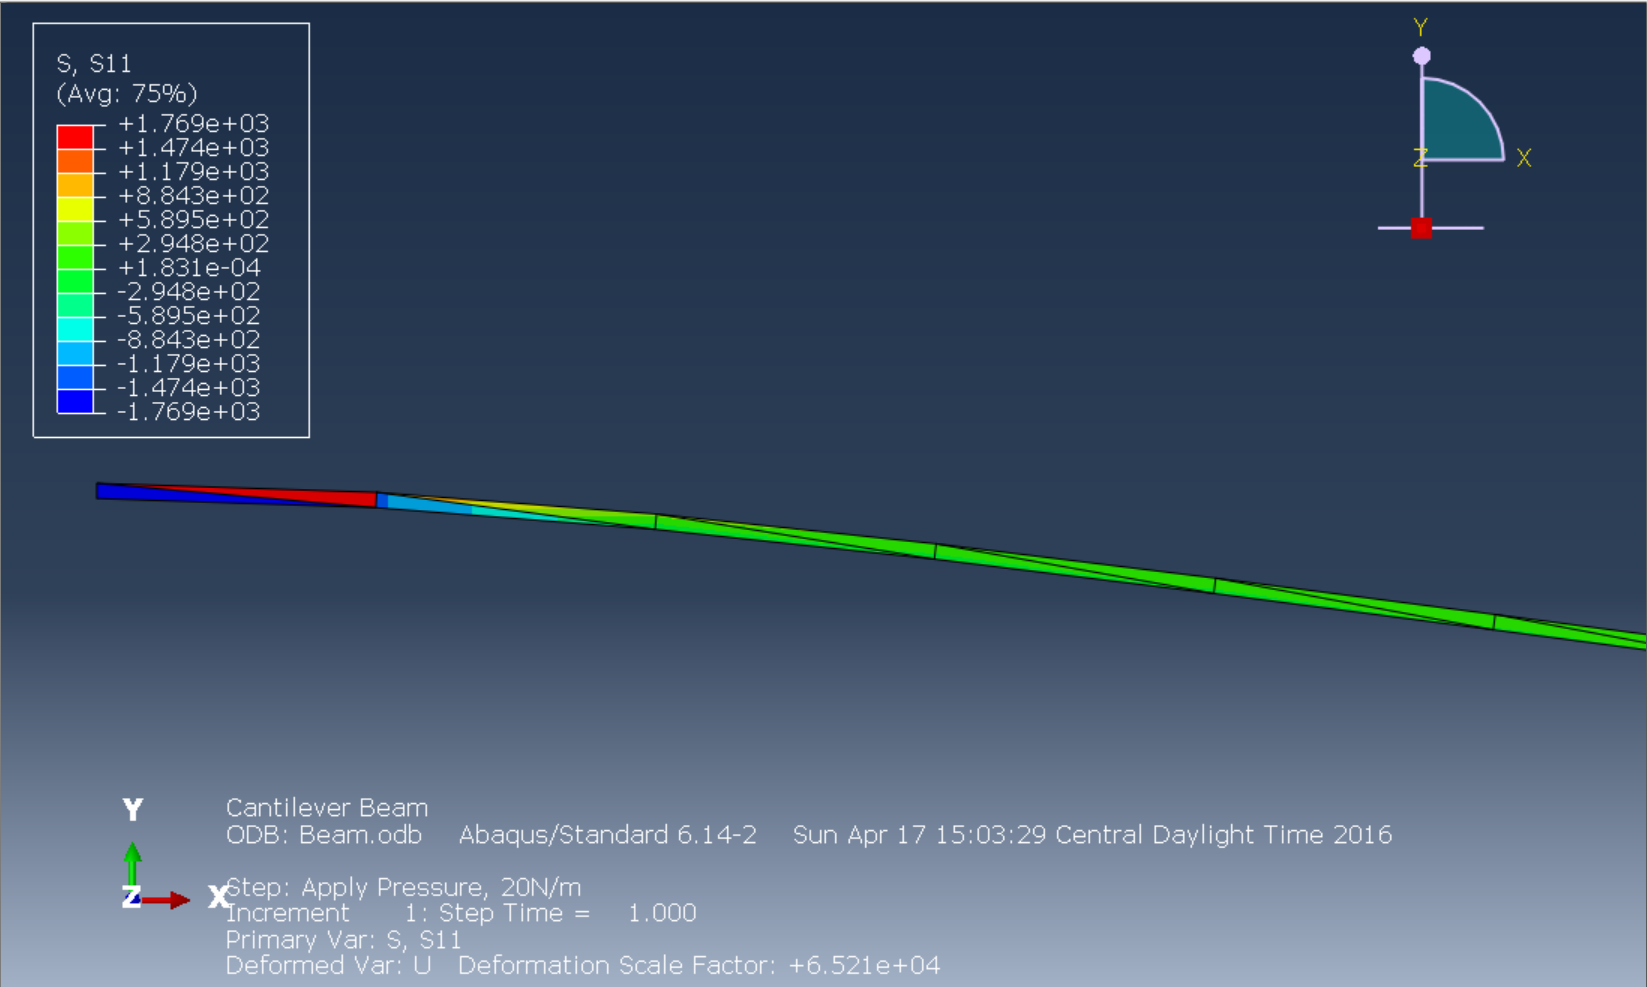
\includegraphics[scale=.50]{3Nsize20stress.PNG}
\caption{Stress Contour, Element Size: 20, Number of Nodes: 14, Number of Elements: 12}
\end{figure}
\begin{figure}[ht]
\centering
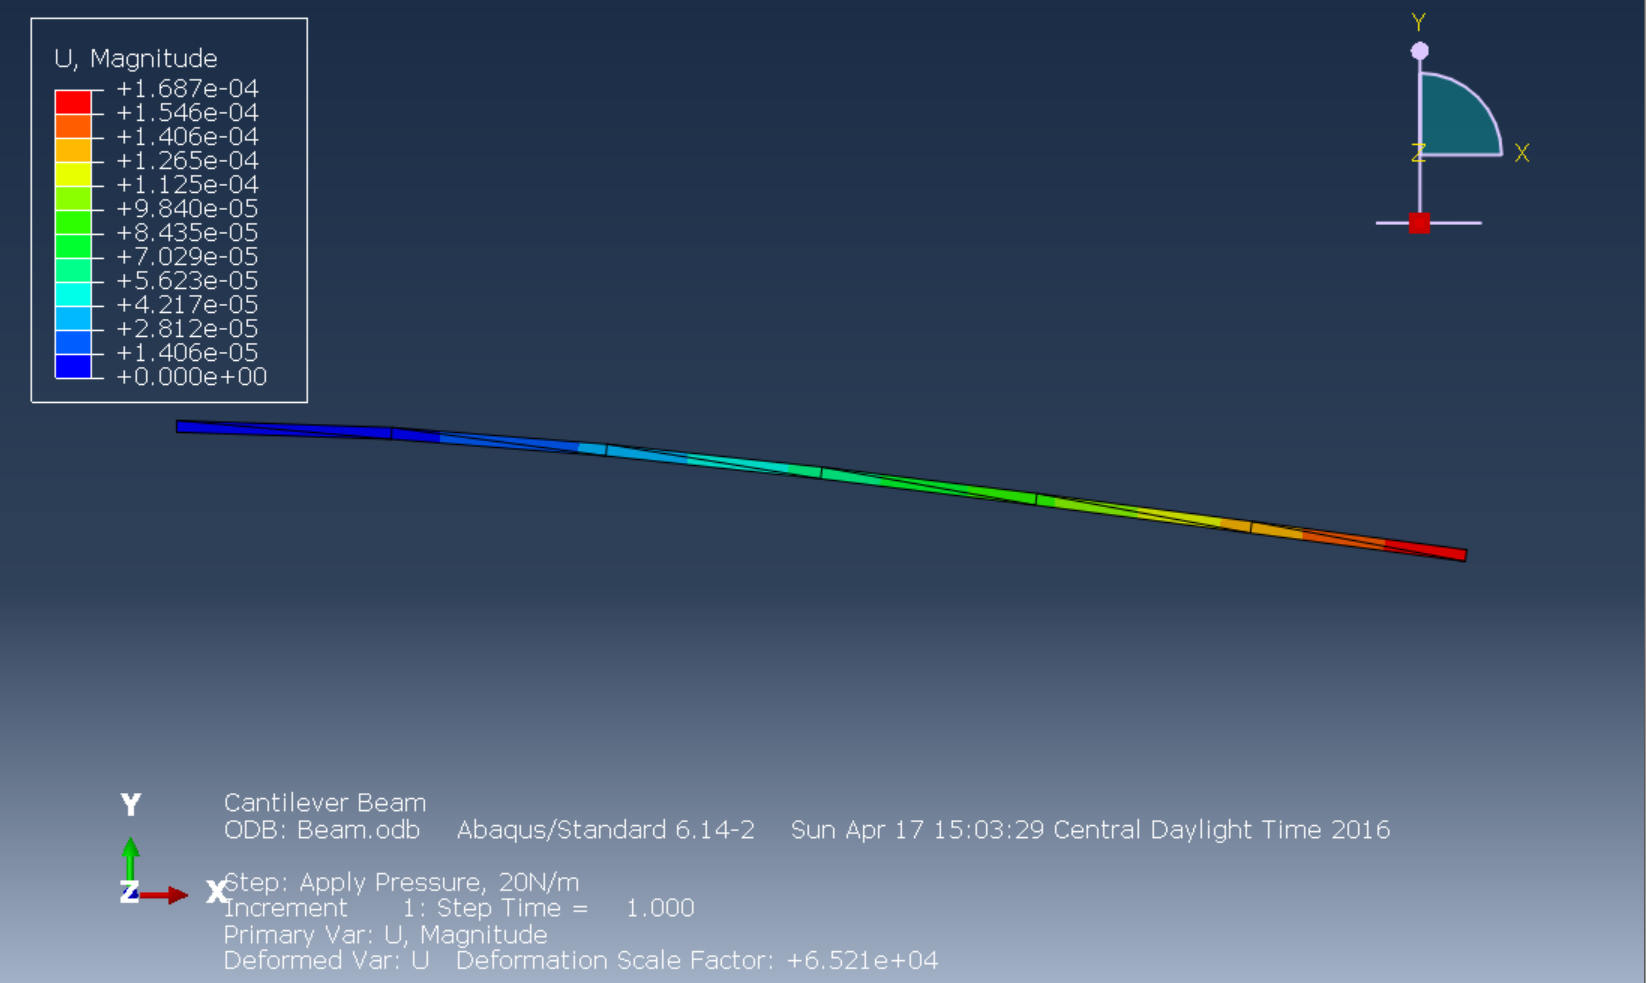
\includegraphics[scale=.50]{3Nsize20MDisplacement.PNG}
\caption{Deflection Contour, Element Size: 20, Number of Nodes: 14, Number of Elements: 12, Maximum Deflection: 168.7 $\mu$m}
\end{figure}

\begin{figure}[ht]
\centering
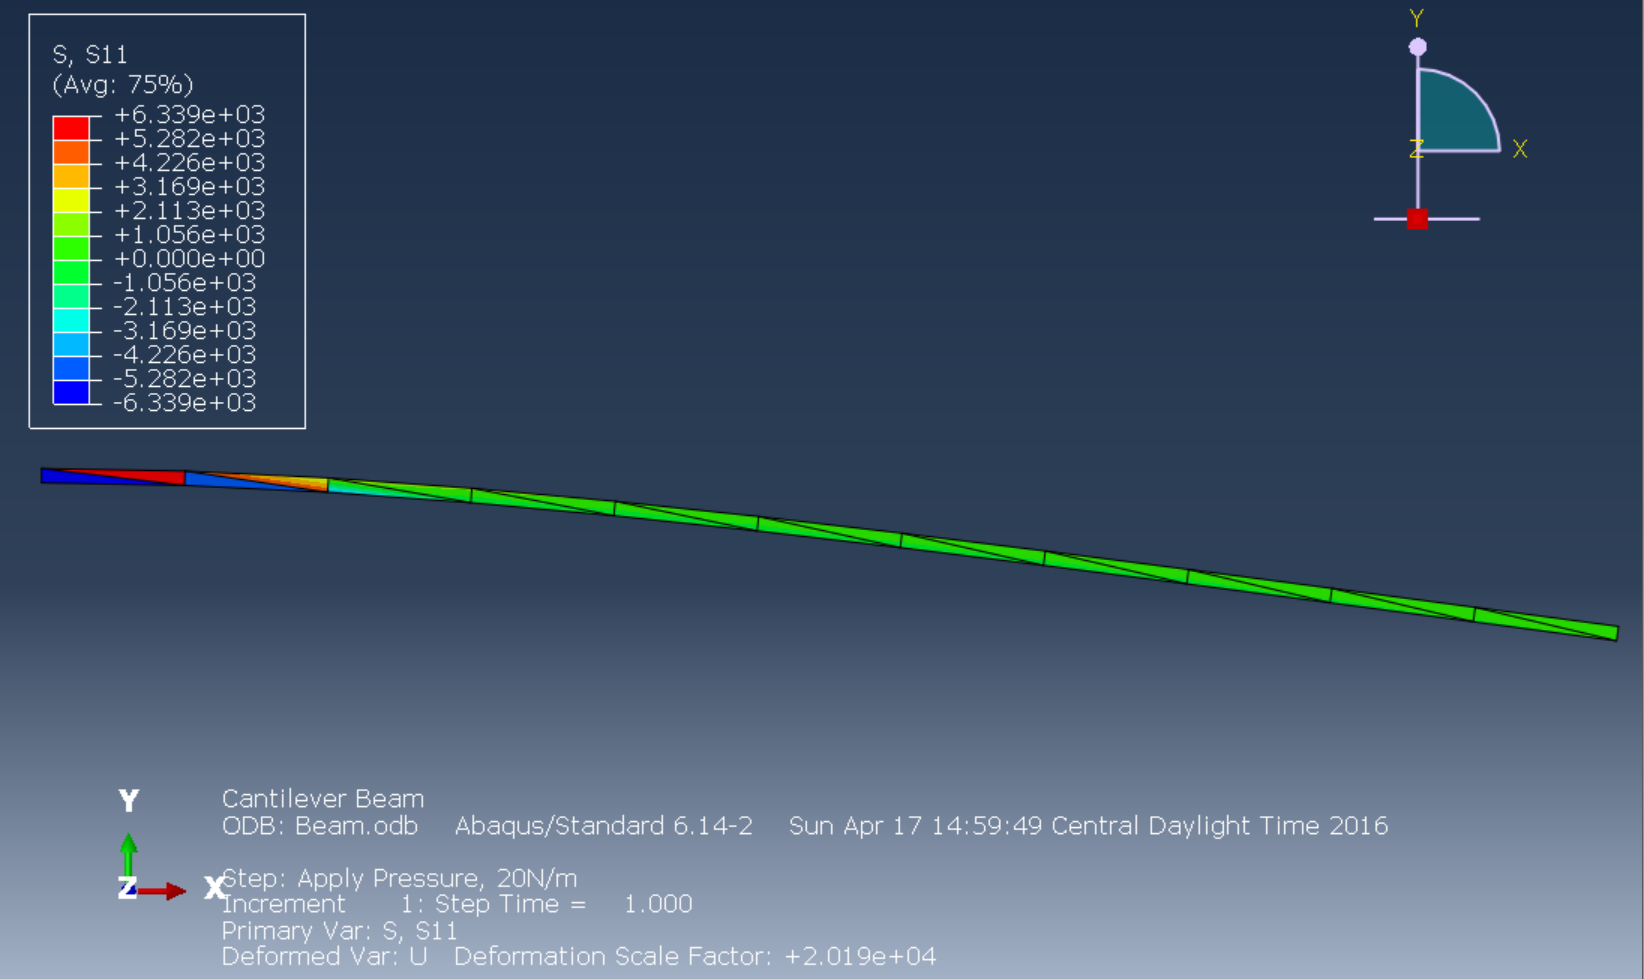
\includegraphics[scale=.50]{3Nsize10Stress.PNG}
\caption{Stress Contour, Element Size: 10, Number of Nodes: 24, Number of Elements: 22}
\end{figure}
\begin{figure}[ht]
\centering
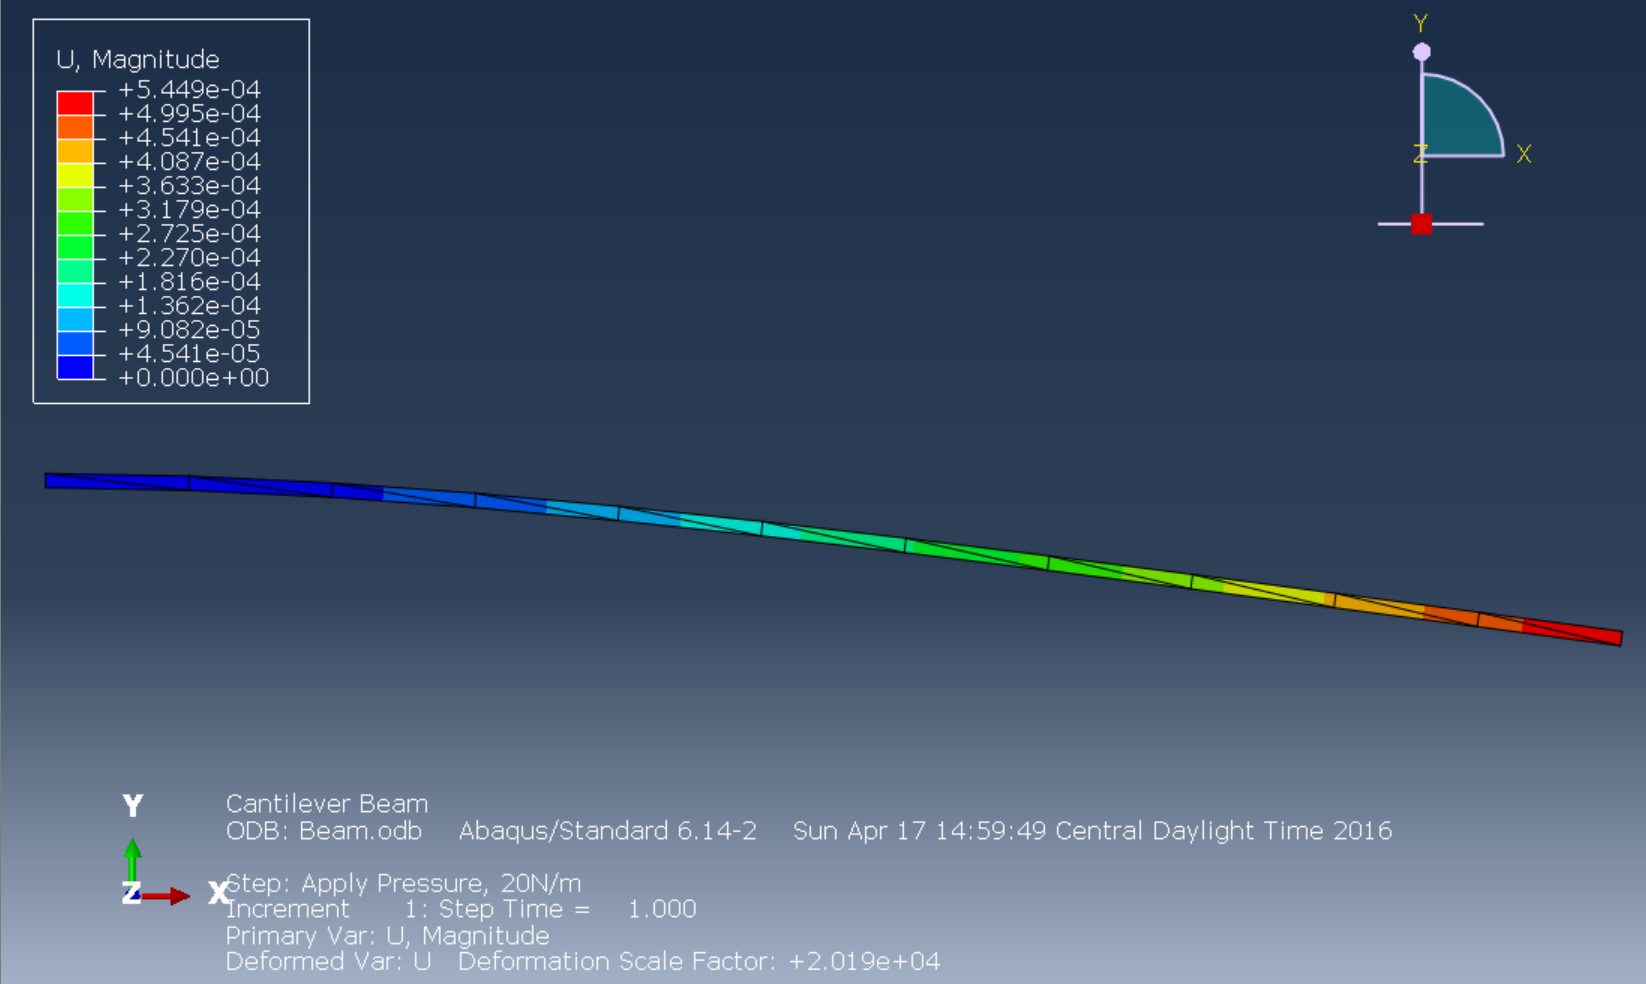
\includegraphics[scale=.50]{3Nsize10MDisplacement.PNG}
\caption{Deflection Contour, Element Size: 10, Number of Nodes: 24, Number of Elements: 22, Maximum Deflection: 544.9 $\mu$m}
\end{figure}

\begin{figure}[ht]
\centering
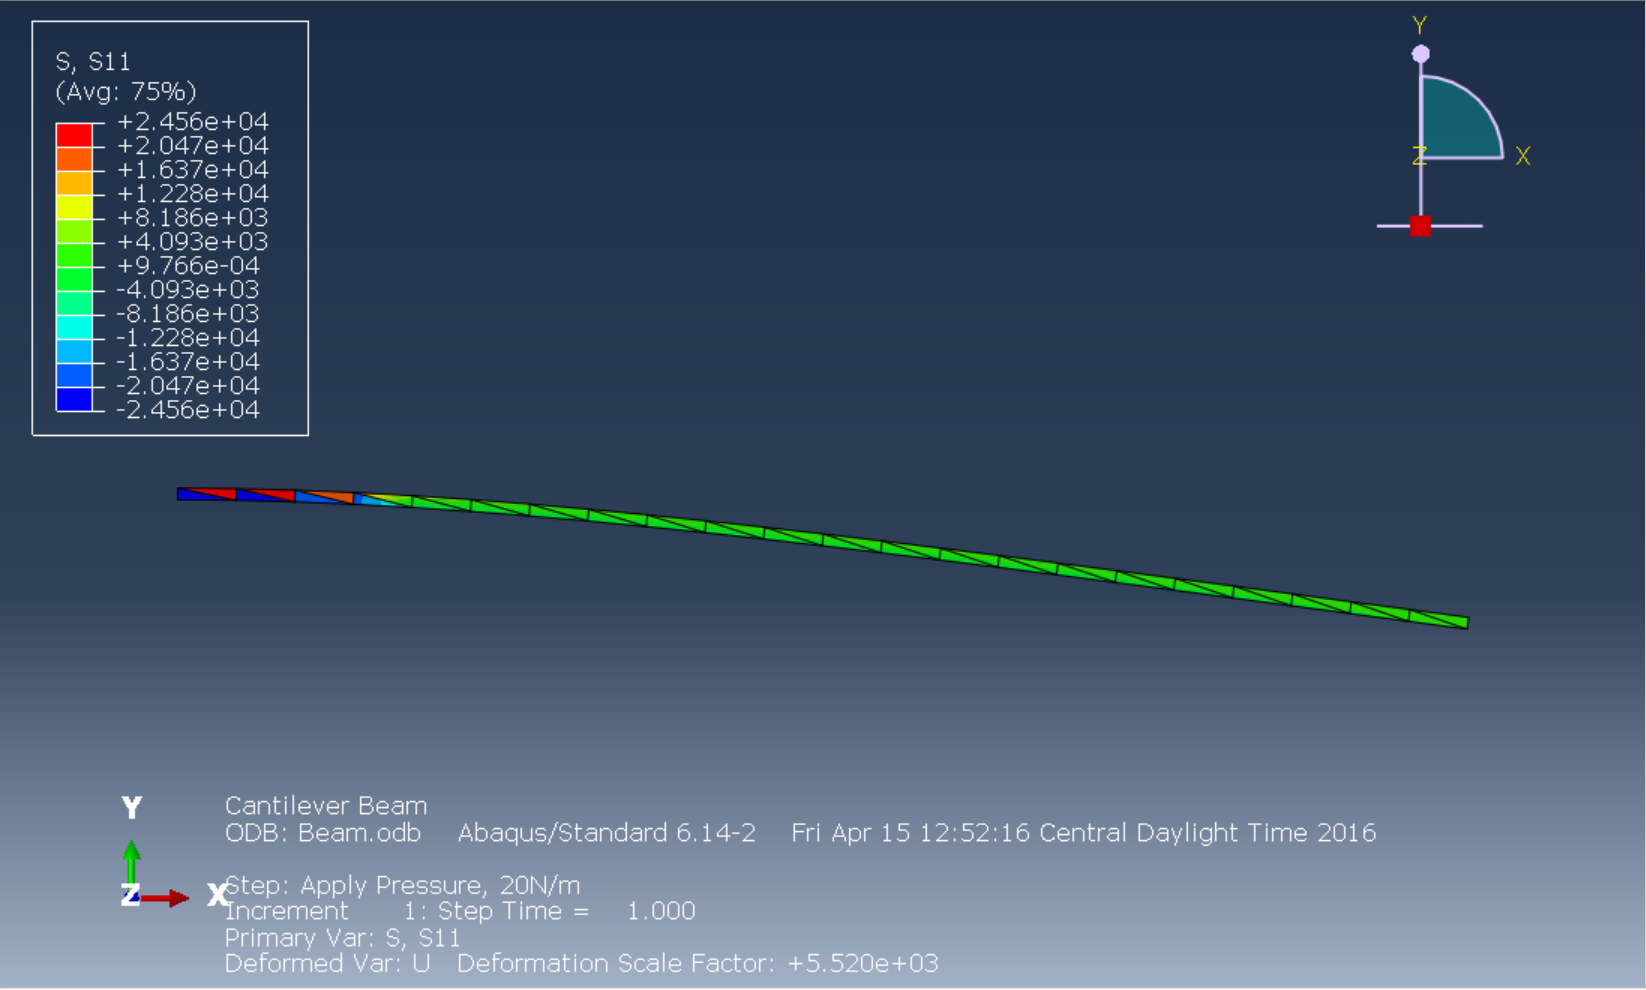
\includegraphics[scale=.50]{3Nsize5Stress.PNG}
\caption{Stress Contour, Element Size: 5, Number of Nodes: 46, Number of Elements: 44}
\end{figure}
\begin{figure}[ht]
\centering
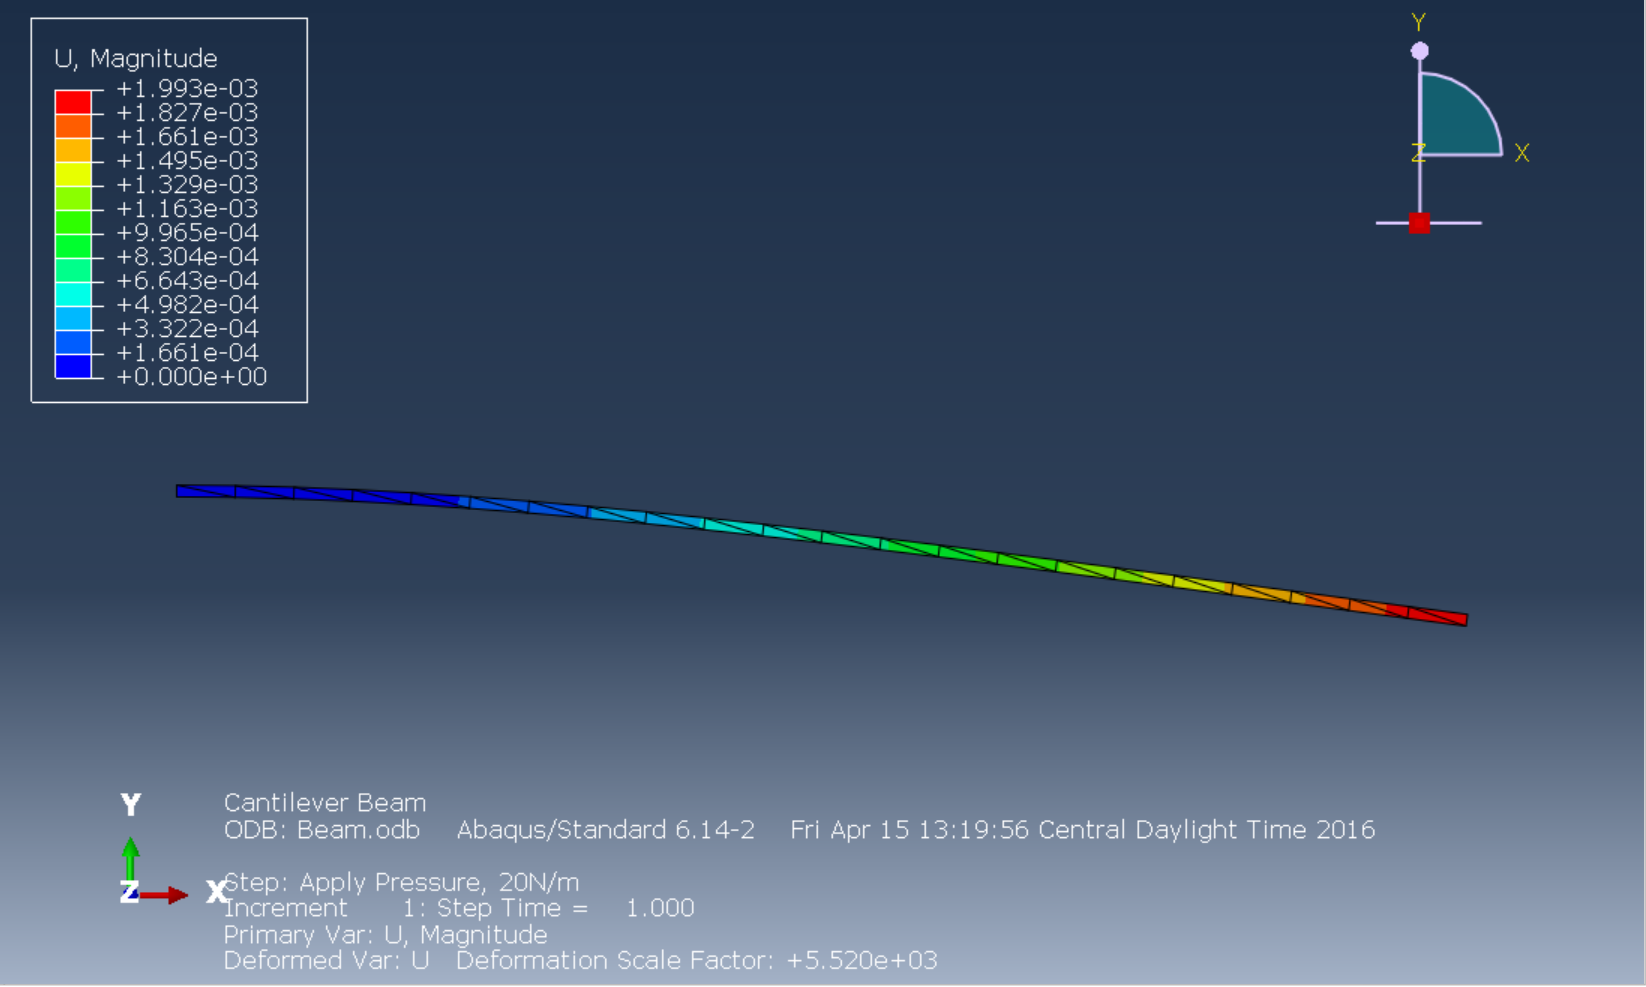
\includegraphics[scale=.50]{3Nsize5MDisplacement.PNG}
\caption{Deflection Contour, Element Size: 5, Number of Nodes: 46, Number of Elements: 44, Maximum Deflection 1.993 mm}
\end{figure}

\begin{figure}[ht]
\centering
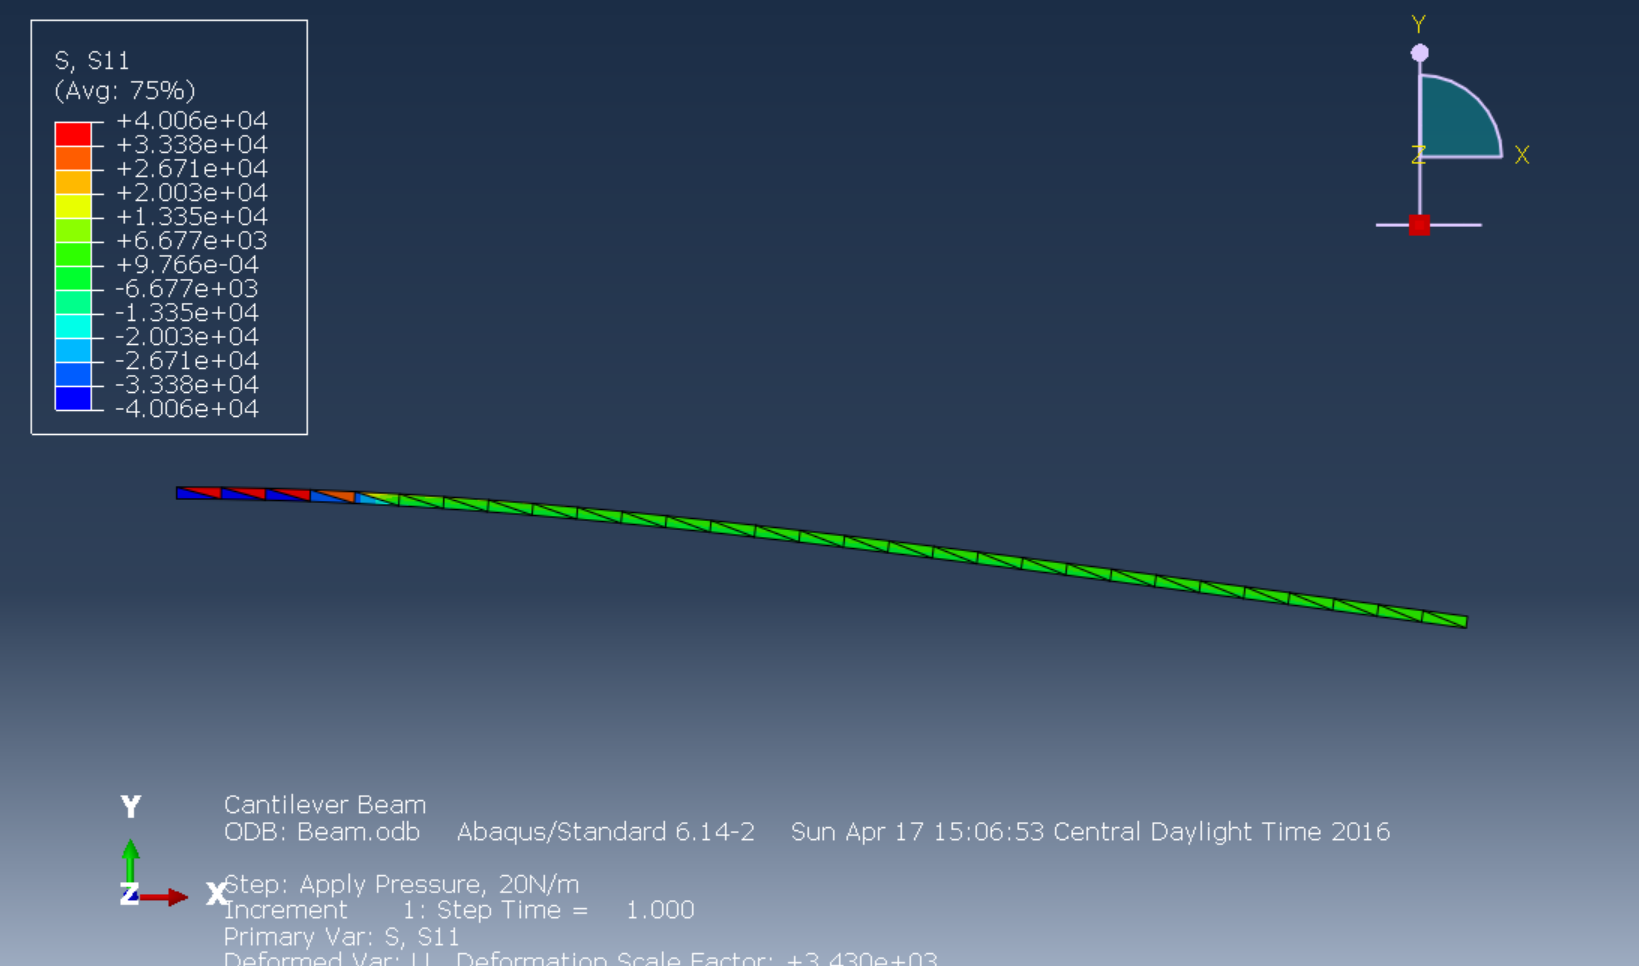
\includegraphics[scale=.50]{3Nsize3_75Stress.PNG}
\caption{Stress Contour, Element Size: 3.75, Number of Nodes: 60, Number of Elements: 58}
\end{figure}
\begin{figure}[ht]
\centering
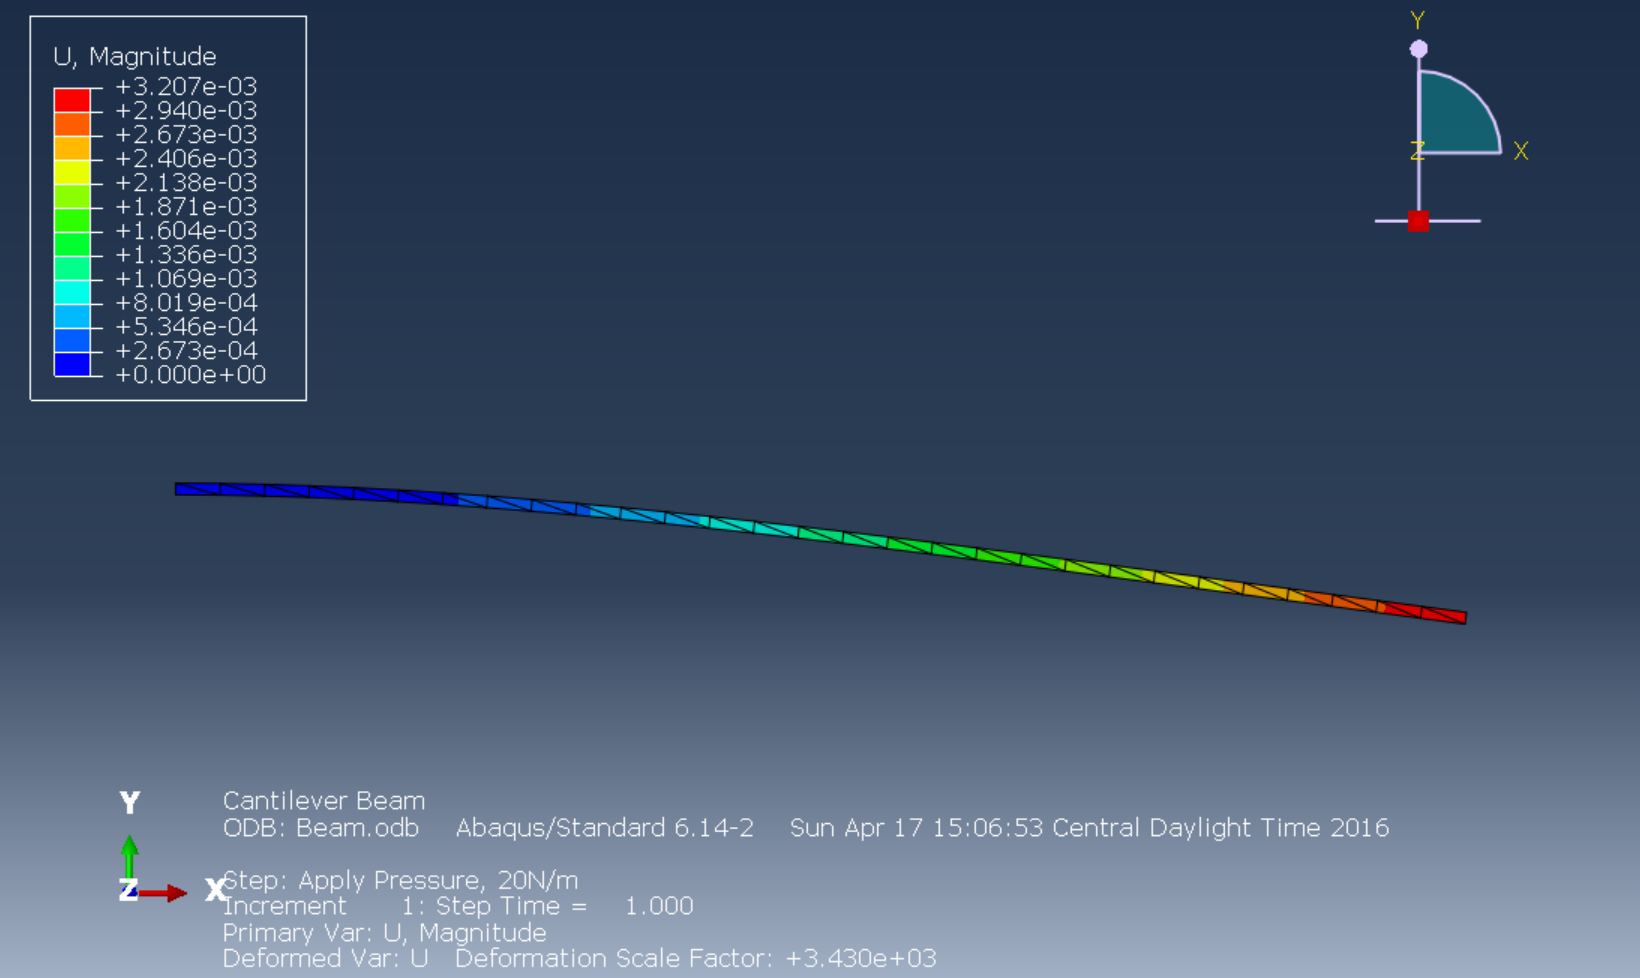
\includegraphics[scale=.50]{3Nsize3_75MDisplacement.PNG}
\caption{Deflection Contour, Element Size: 3.75, Number of Nodes: 60, Number of Elements: 58, Maximum Deflection: 3.207 mm}
\end{figure}

\begin{figure}[ht]
\centering
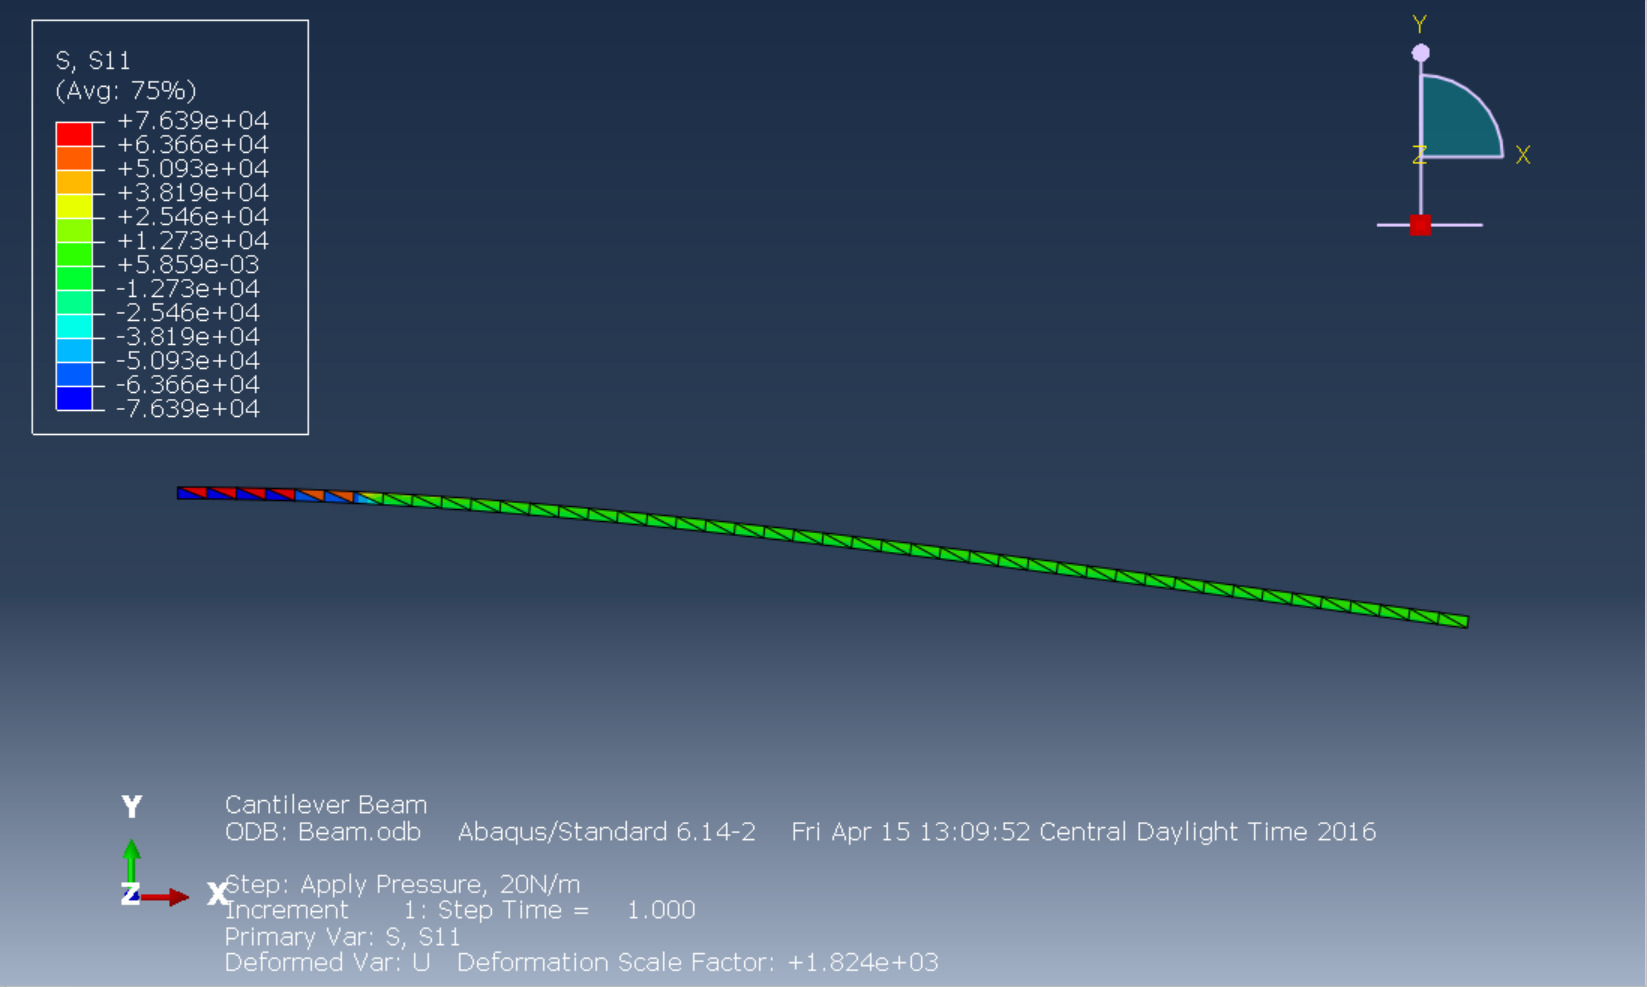
\includegraphics[scale=.50]{3Nsize2_5Stress.PNG}
\caption{Stress Contour, Element Size: 2.5, Number of Nodes: 90, Number of Elements: 88}
\end{figure}
\begin{figure}[ht]
\centering
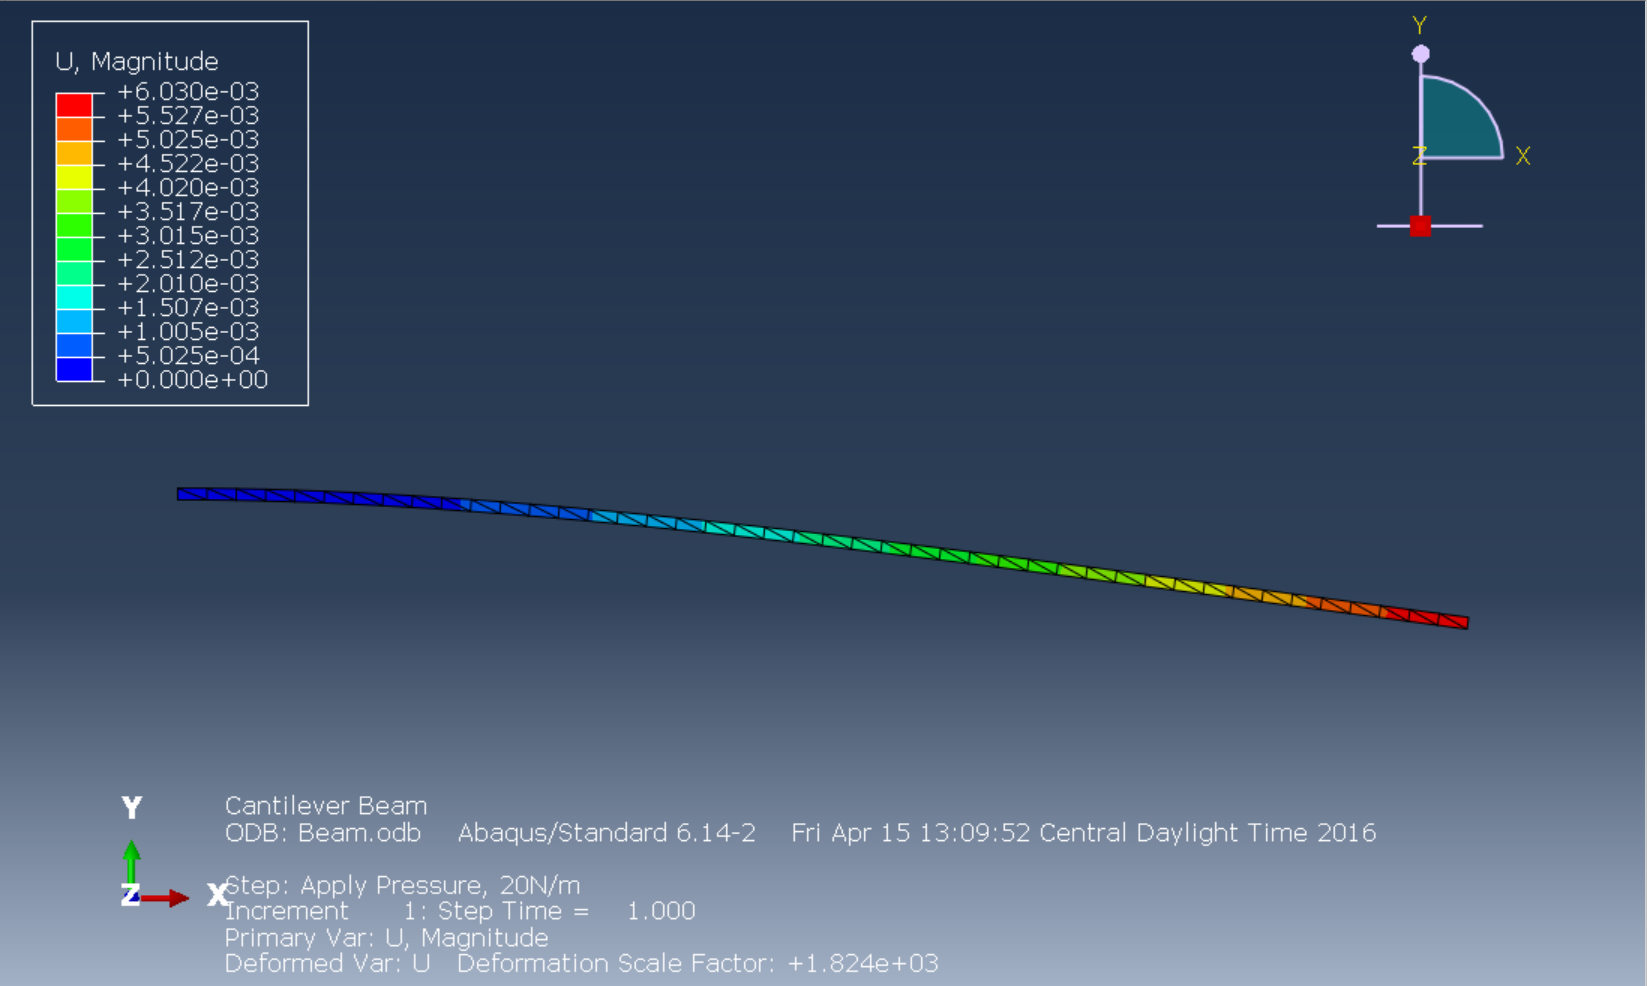
\includegraphics[scale=.50]{3Nsize2_5MDisplacement.PNG}
\caption{Deflection Contour, Element Size: 2.5, Number of Nodes: 90, Number of Elements: 88, Maximum Deflection: 6.030 mm}
\end{figure}

\begin{figure}[ht]
\centering
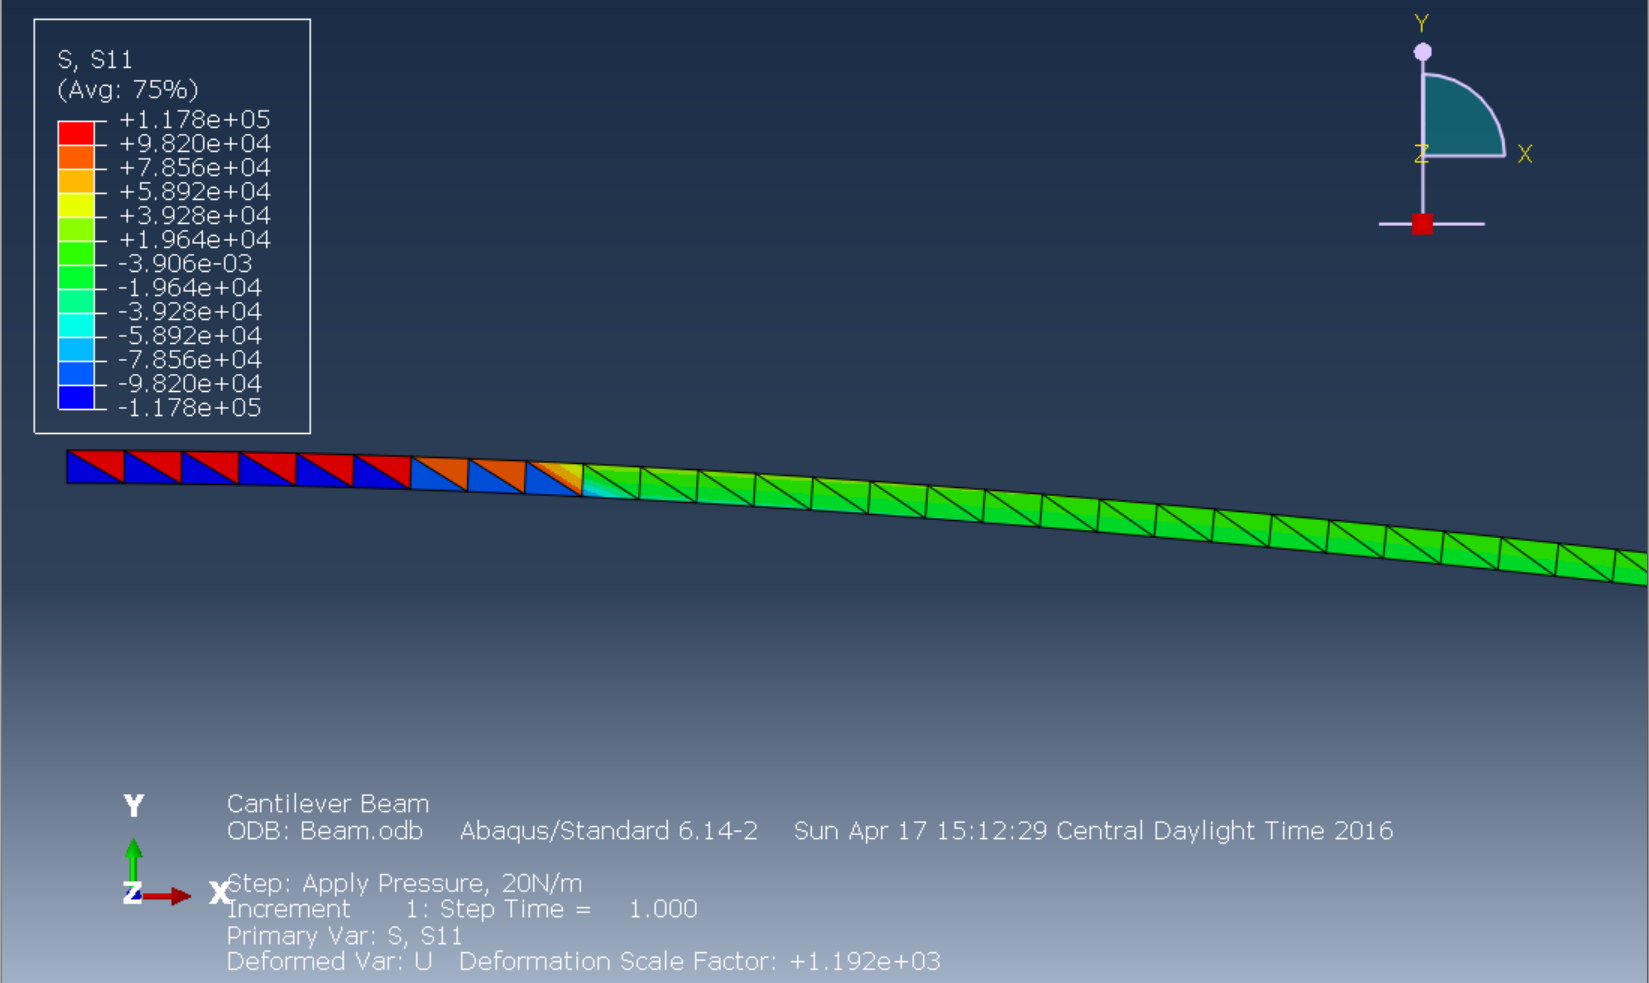
\includegraphics[scale=.50]{3Nsize1_75Stress.PNG}
\caption{Stress Contour, Element Size: 1.75, Number of Nodes: 128, Number of Elements: 126}
\end{figure}
\begin{figure}[ht]
\centering
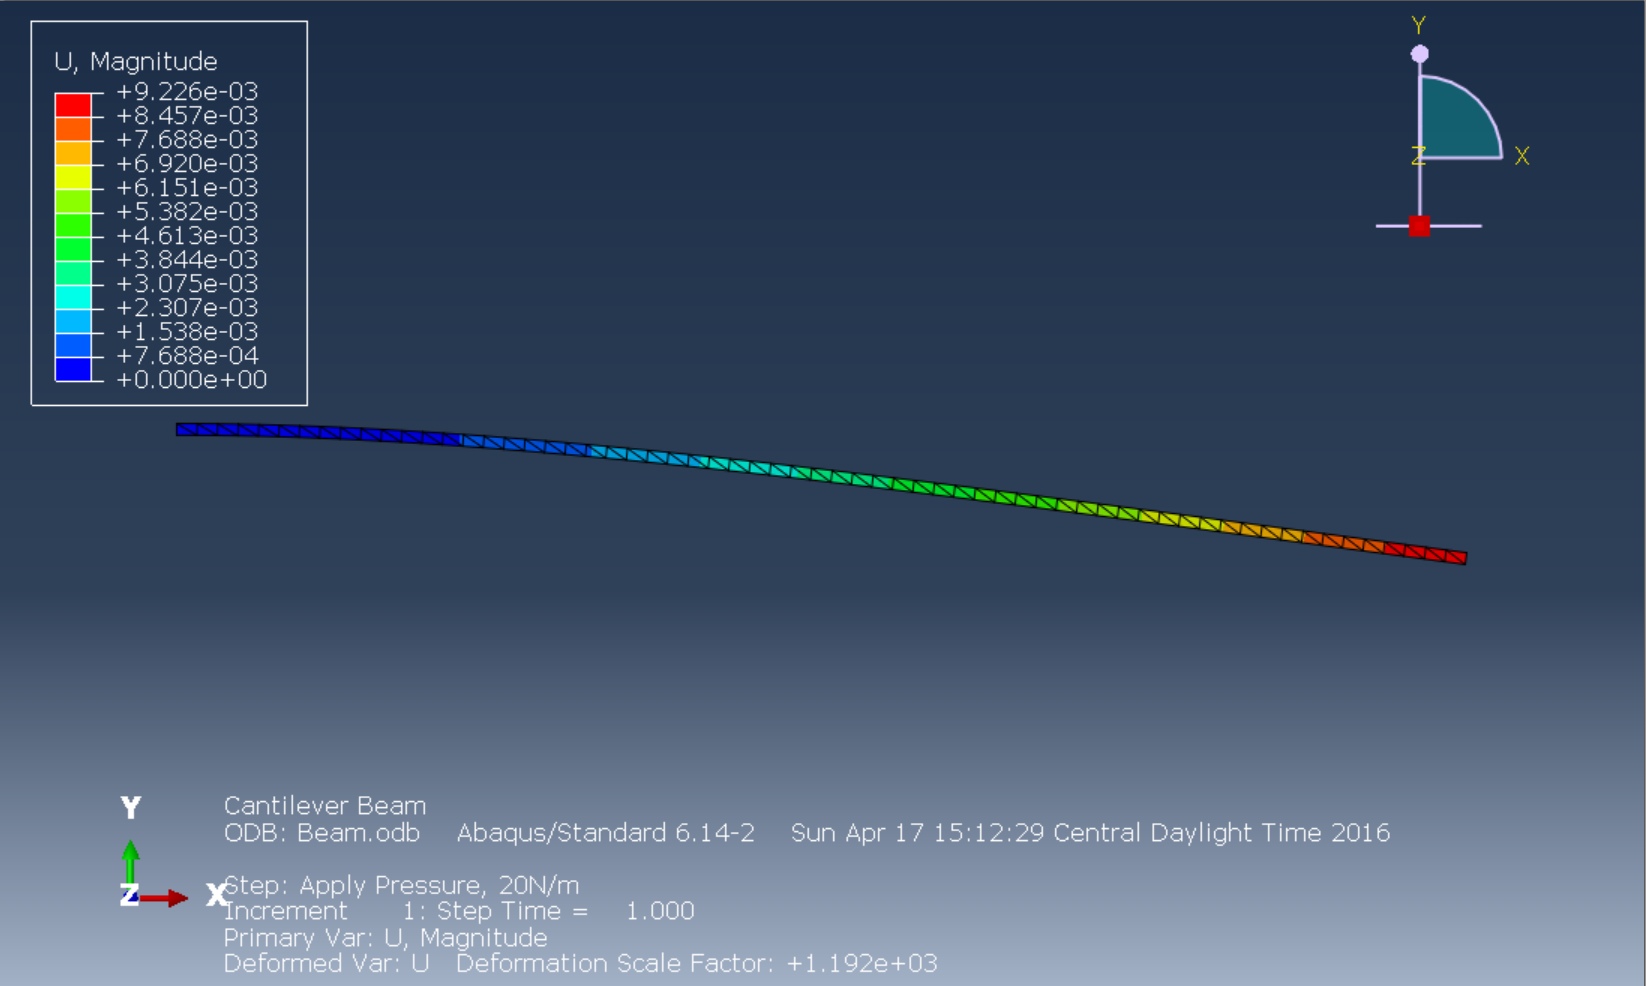
\includegraphics[scale=.50]{3Nsize1_75MDisplacement.PNG}
\caption{Deflection Contour, Element Size: 1.75, Number of Nodes: 128, Number of Elements: 126, Maximum Deflection: 9.226 mm}
\end{figure}

\begin{figure}[ht]
\centering
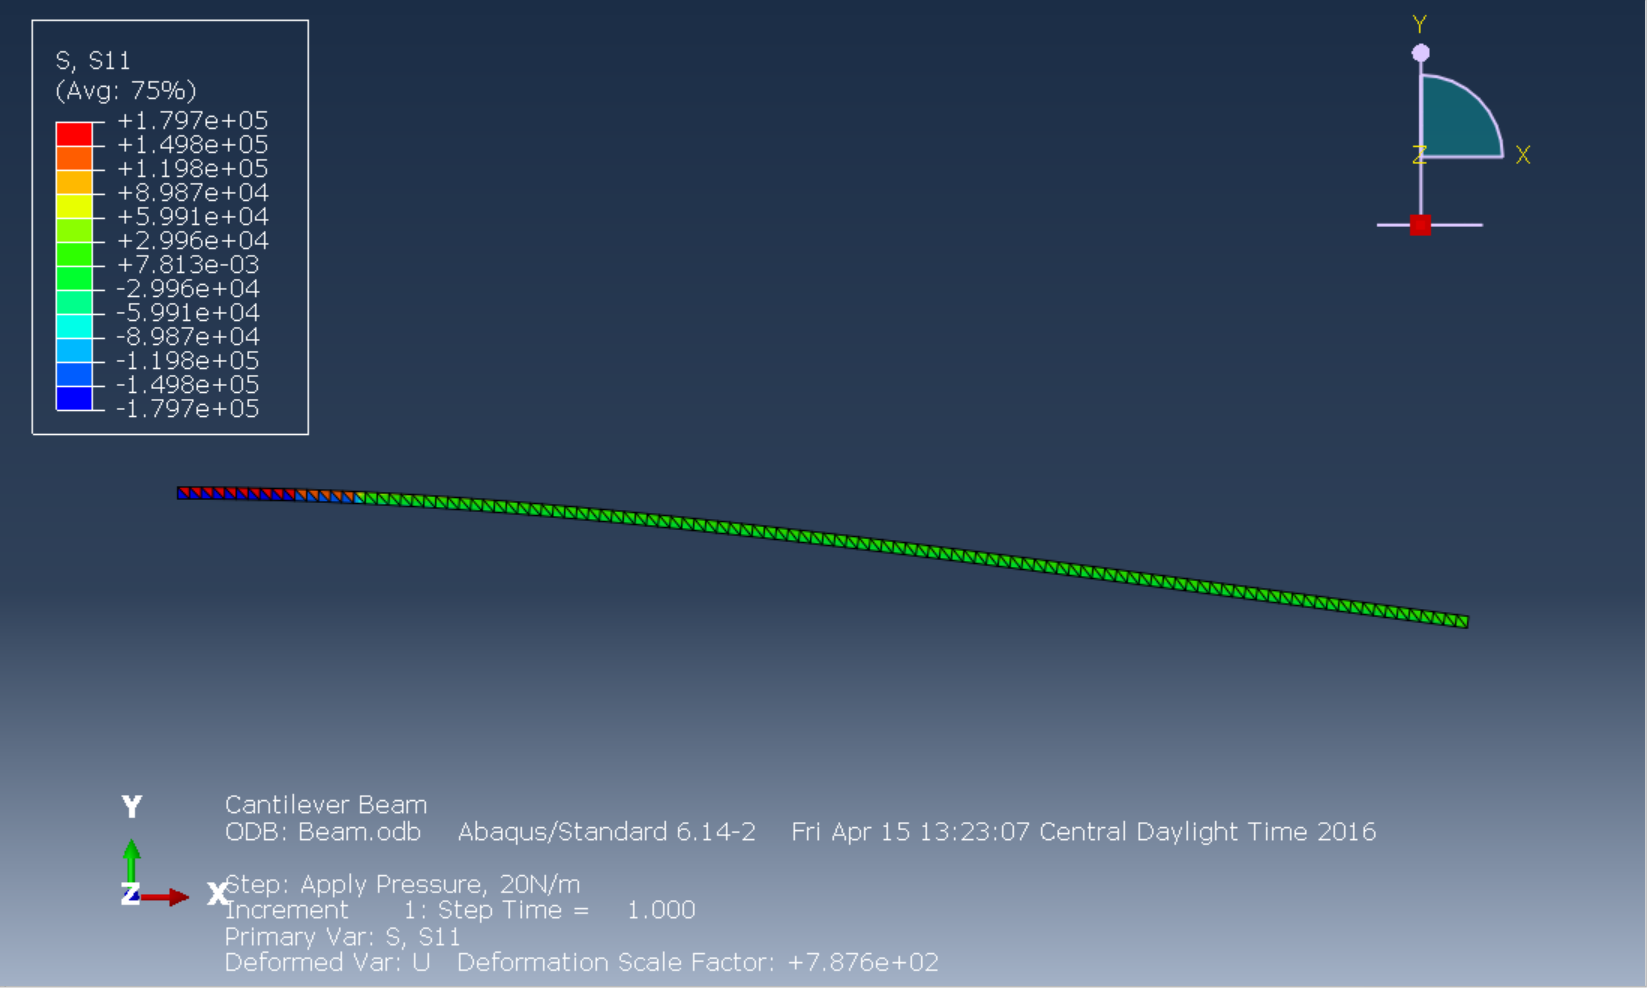
\includegraphics[scale=.50]{3Nsize1Stress.PNG}
\caption{Stress Contour, Element Size: 1, Number of Nodes: 222, Number of Elements: 220}
\end{figure}
\begin{figure}[ht]
\centering
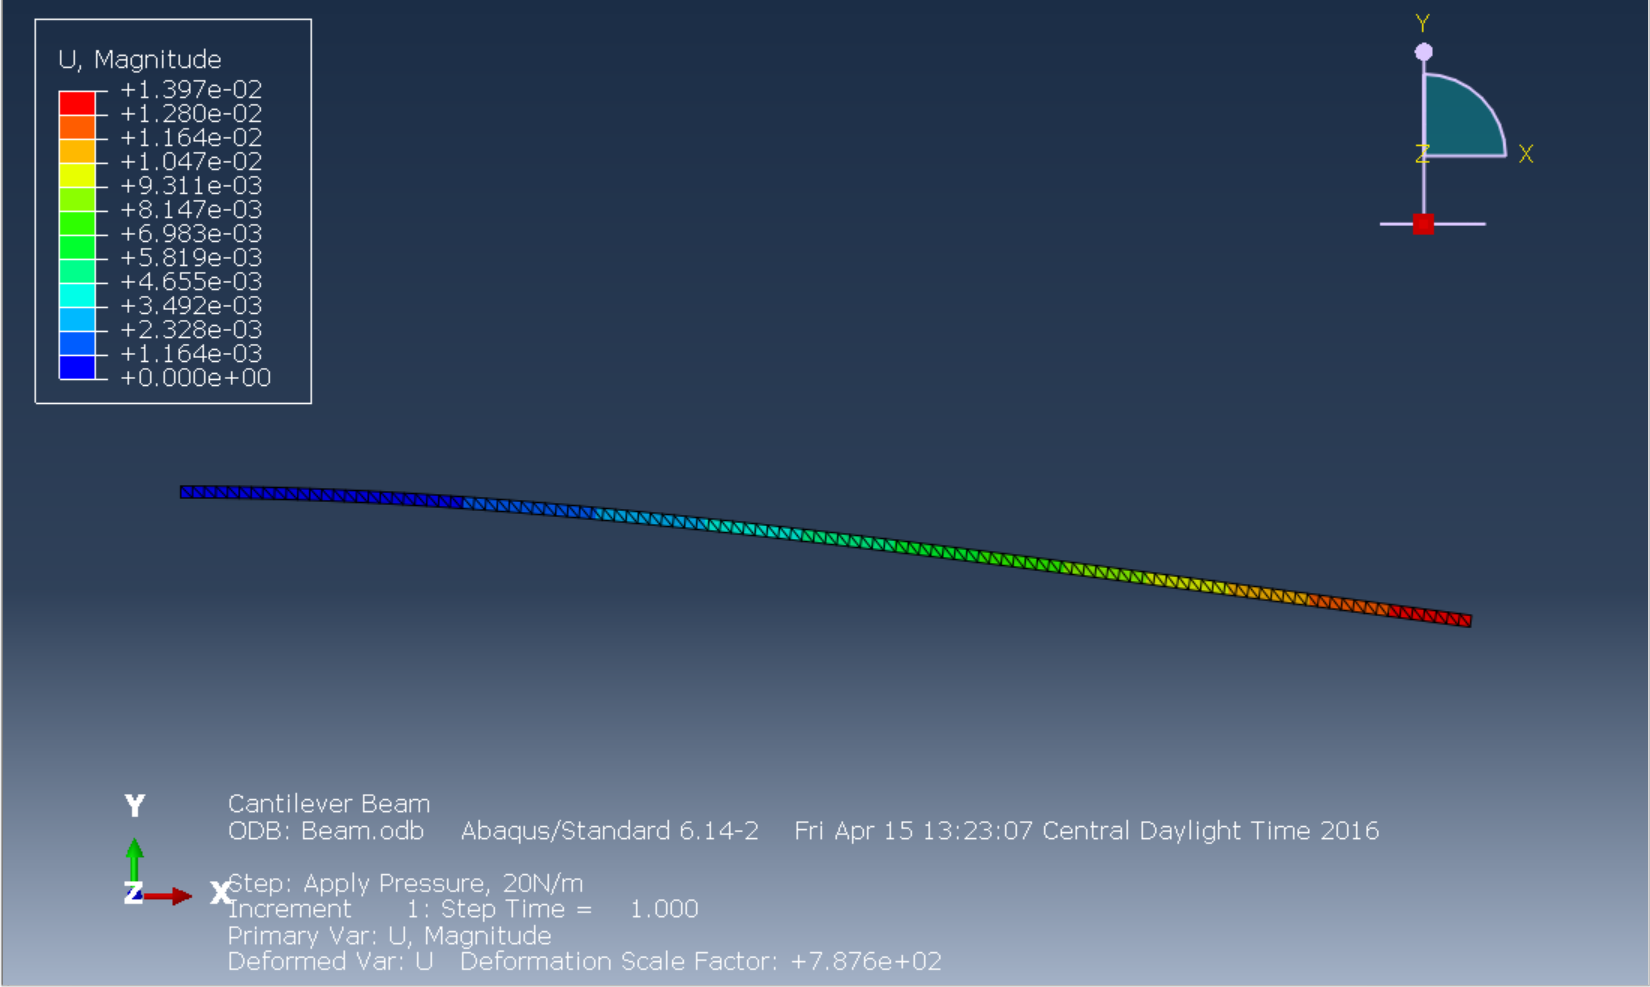
\includegraphics[scale=.50]{3Nsize1MDisplacement.PNG}
\caption{Deflection Contour, Element Size: 1, Number of Nodes: 222, Number of Elements: 220, Maximum Deflection: 1.397 cm}
\end{figure}

\begin{figure}[ht]
\centering
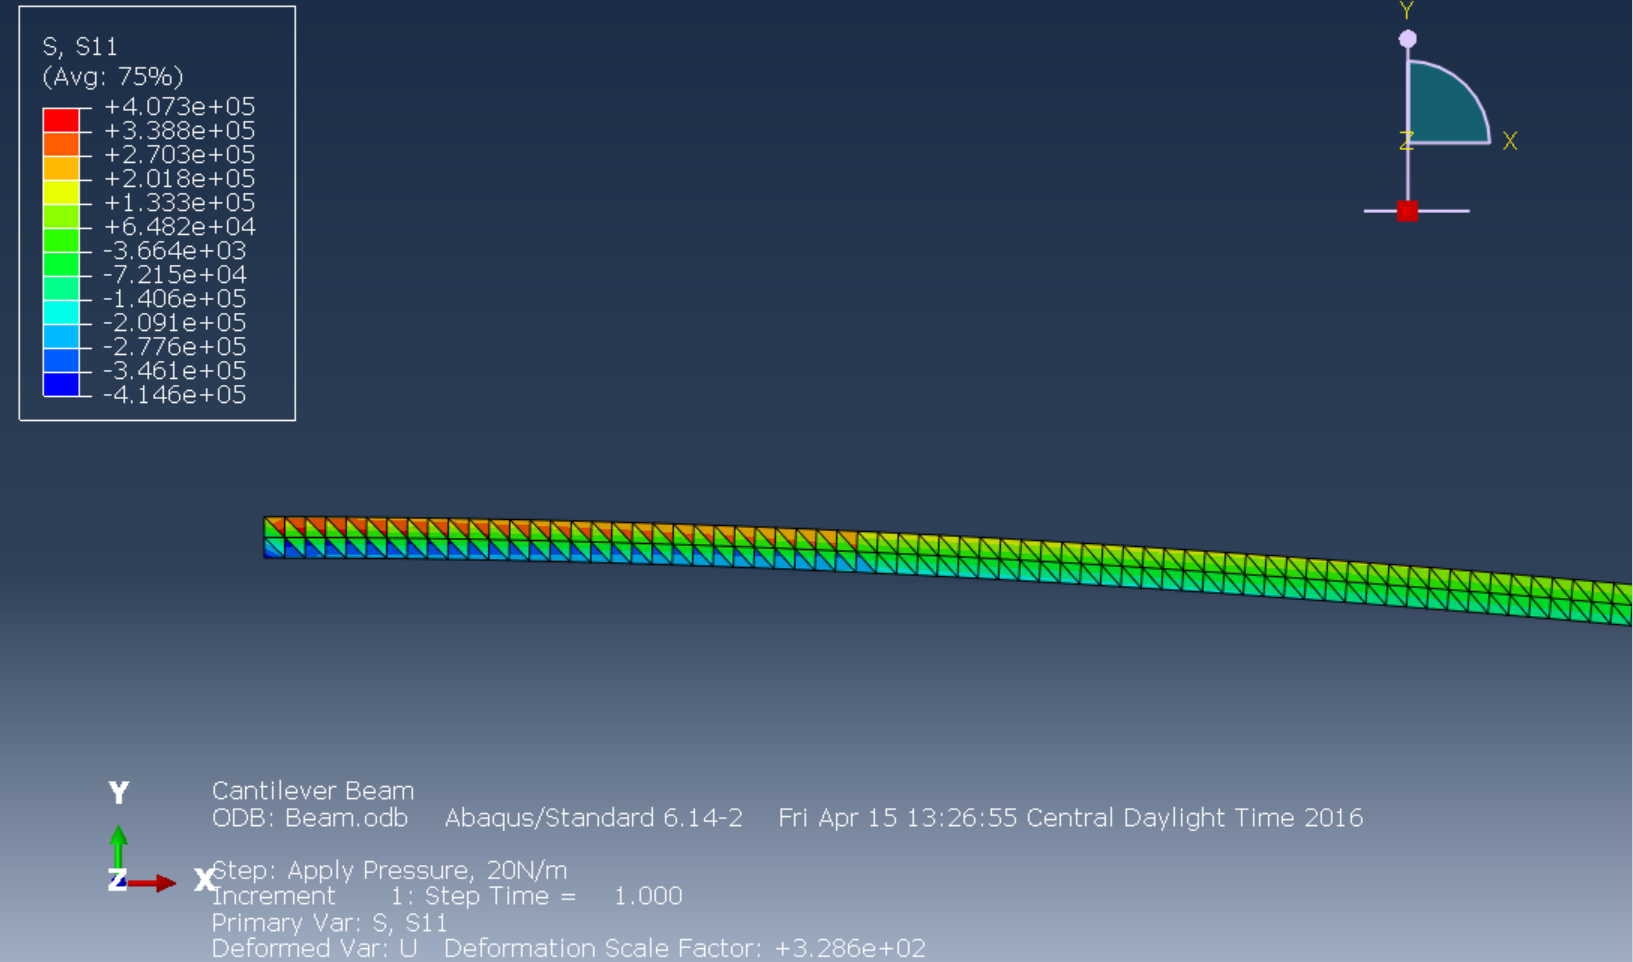
\includegraphics[scale=.50]{3Nsize0_5StressClose.PNG}
\caption{Stress Contour, Element Size: 0.5, Number of Nodes: 663, Number of Elements: 880}
\end{figure}
\begin{figure}[ht]
\centering
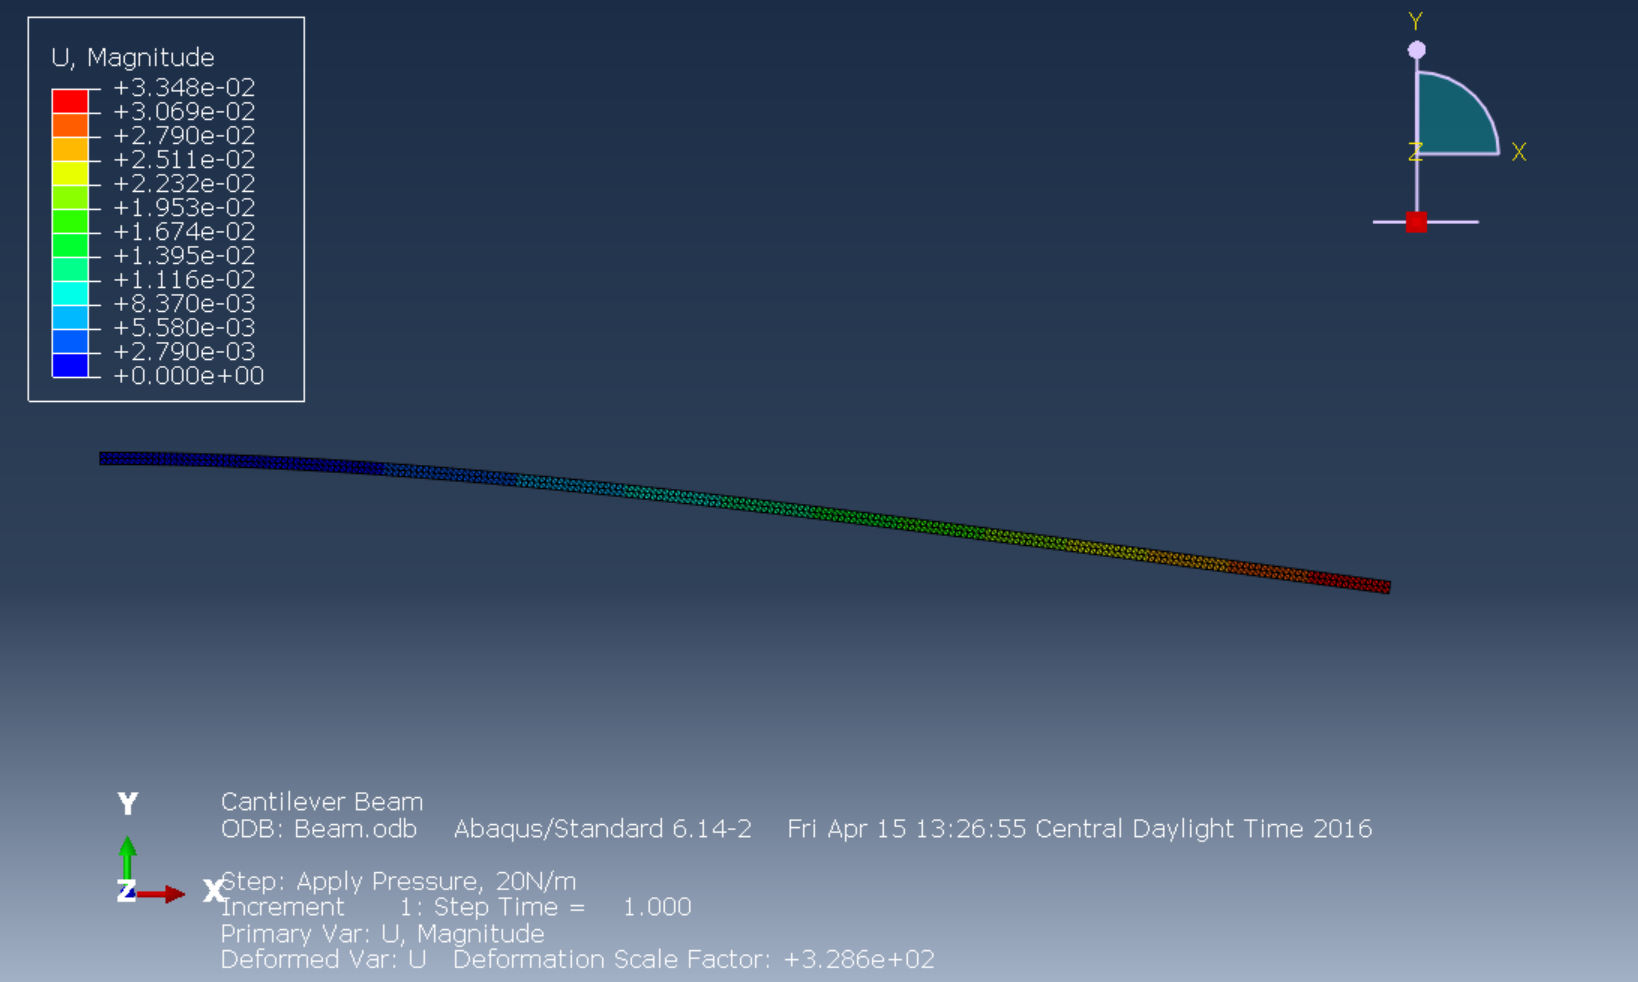
\includegraphics[scale=.50]{3Nsize0_5MDisplacement.PNG}
\caption{Deflection Contour, Element Size: 0.5, Number of Nodes: 663, Number of Elements: 880, Maximum Deflection: 3.348 cm}
\end{figure}

\extrafloats{100}

\begin{figure}[ht]
\centering
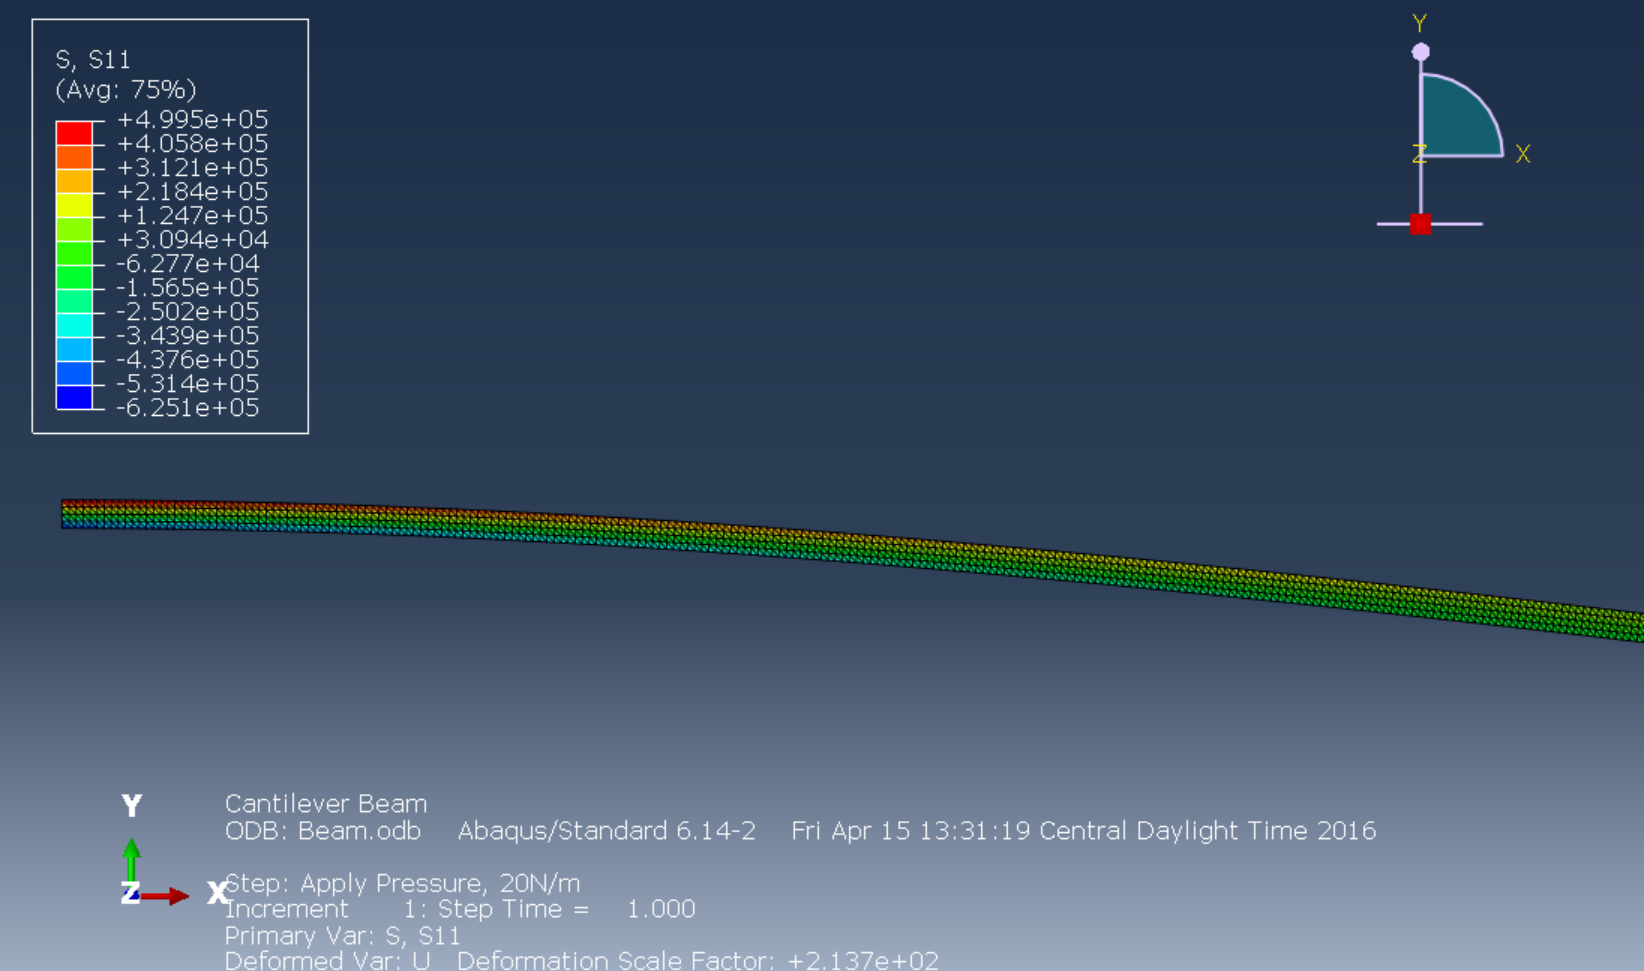
\includegraphics[scale=.50]{3Nsize0_25Stress.PNG}
\caption{Stress Contour, Element Size: 0.25, Number of Nodes: 2205, Number of Elements: 3520}
\end{figure}
\begin{figure}[ht]
\centering
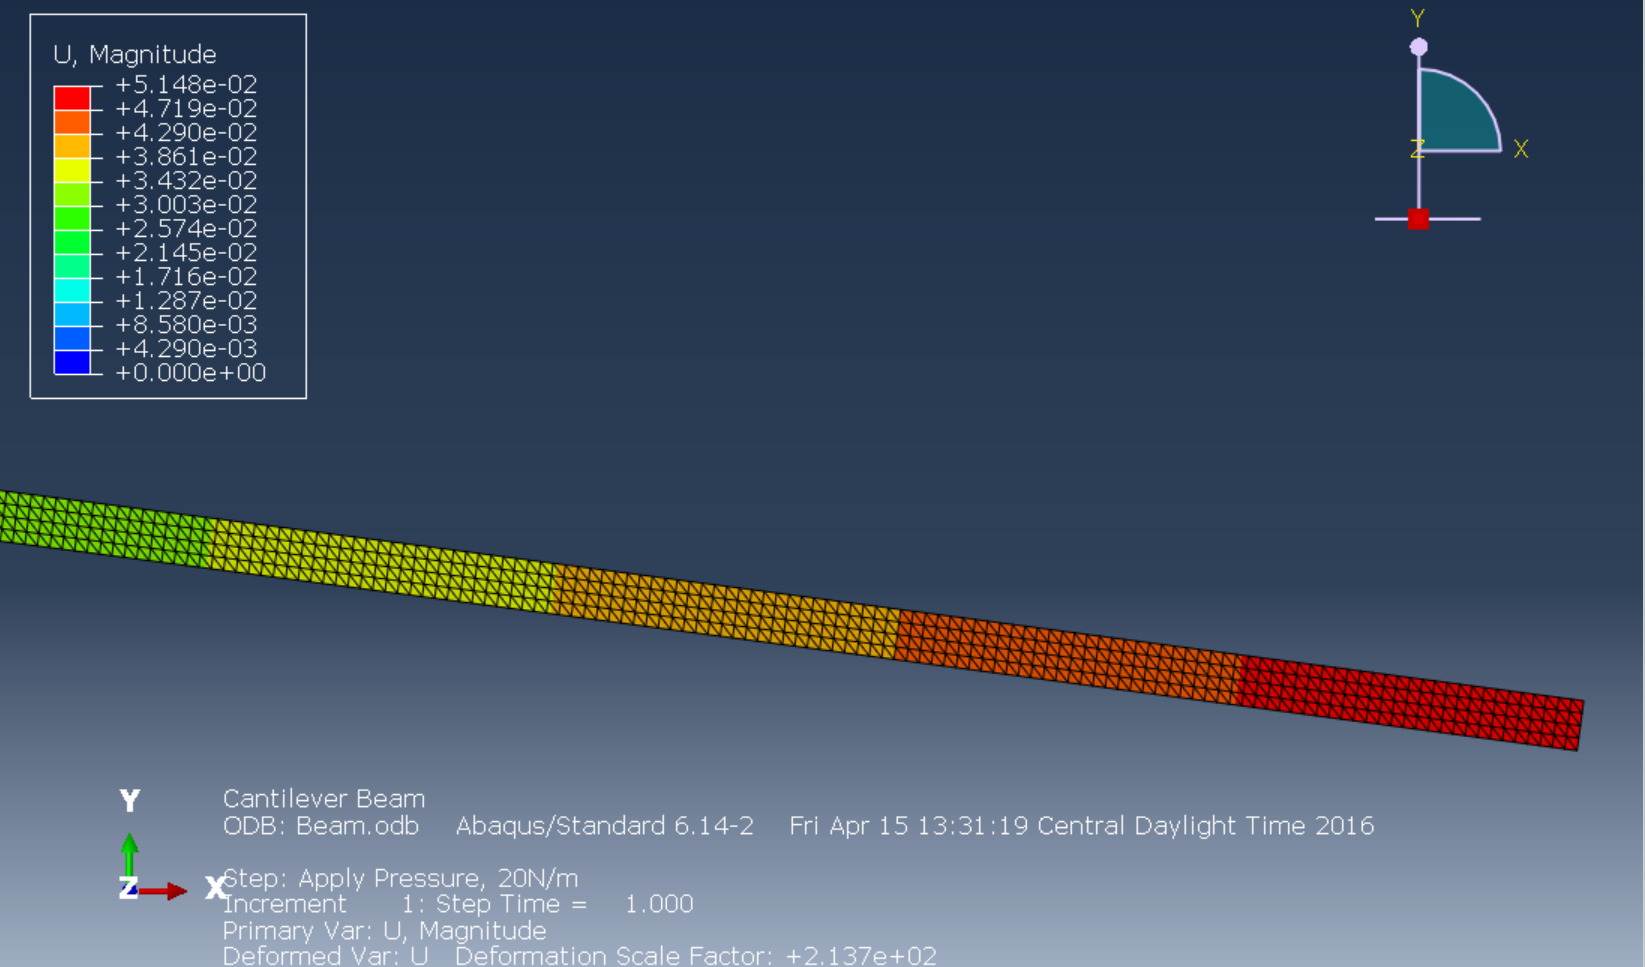
\includegraphics[scale=.50]{3Nsize0_25MDisplacement.PNG}
\caption{Deflection Contour, Element Size: 0.25, Number of Nodes: 2205, Number of Elements: 3520, Maximum Deflection: 5.148 cm}
\end{figure}

\begin{figure}[ht]
\centering
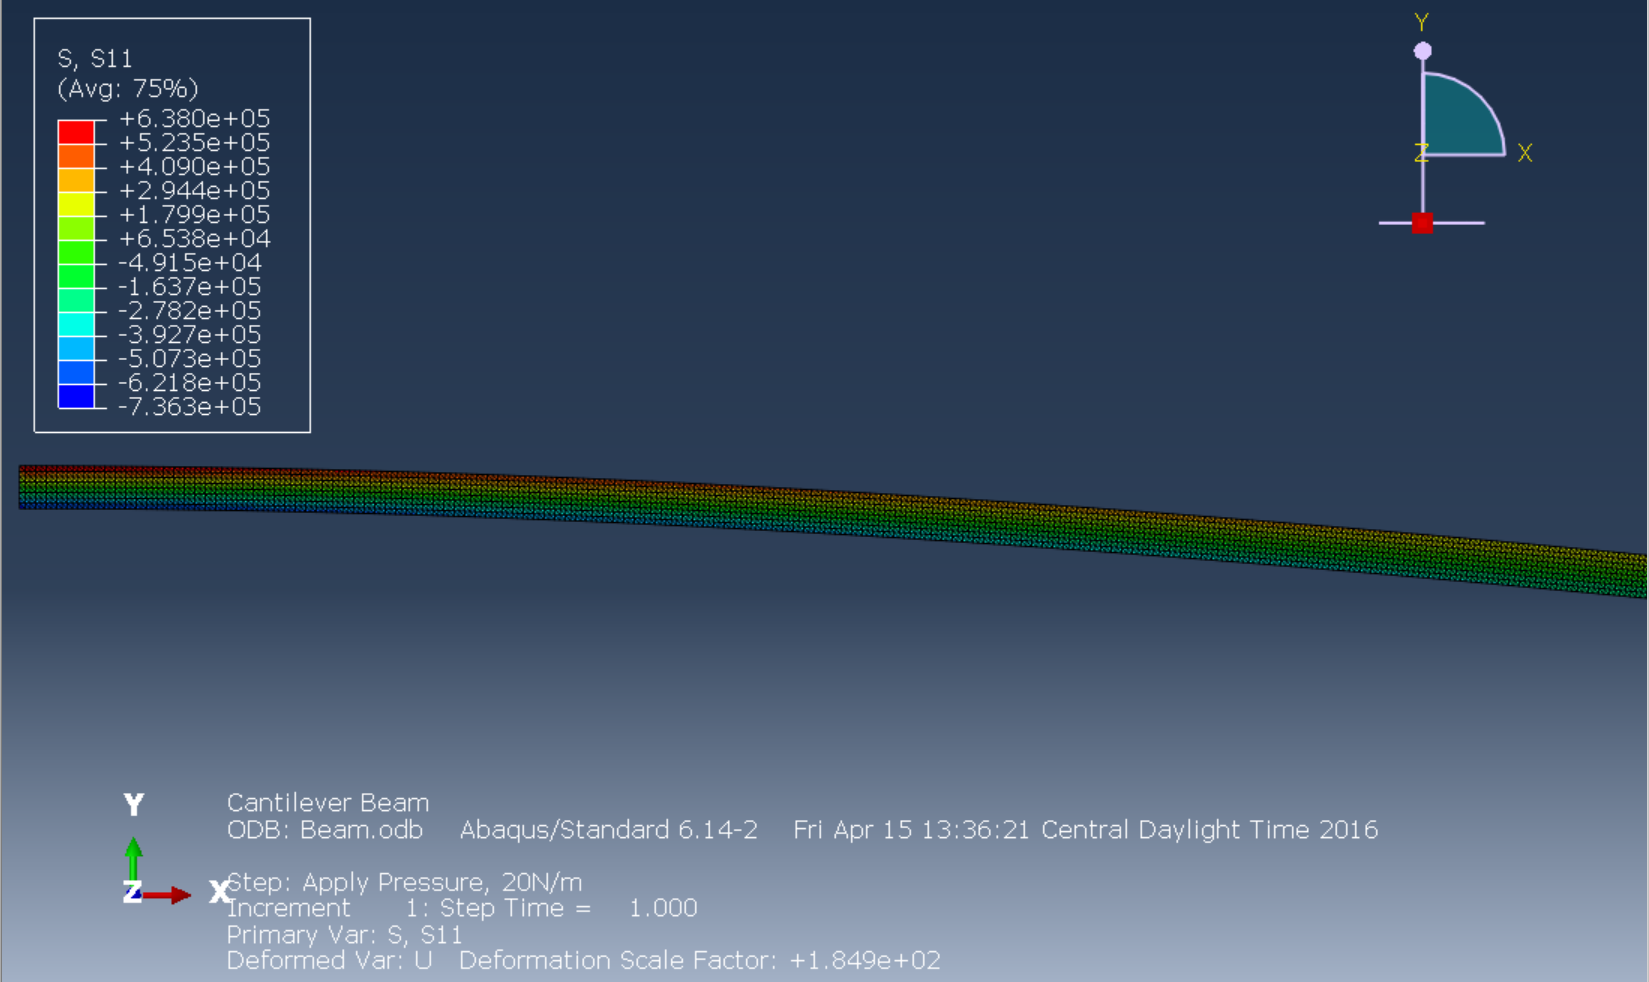
\includegraphics[scale=.50]{3Nsize0_125Stress.PNG}
\caption{Stress Contour, Element Size: 0.125, Number of Nodes: 7929, Number of Elements: 14,080}
\end{figure}
\begin{figure}[ht]
\centering
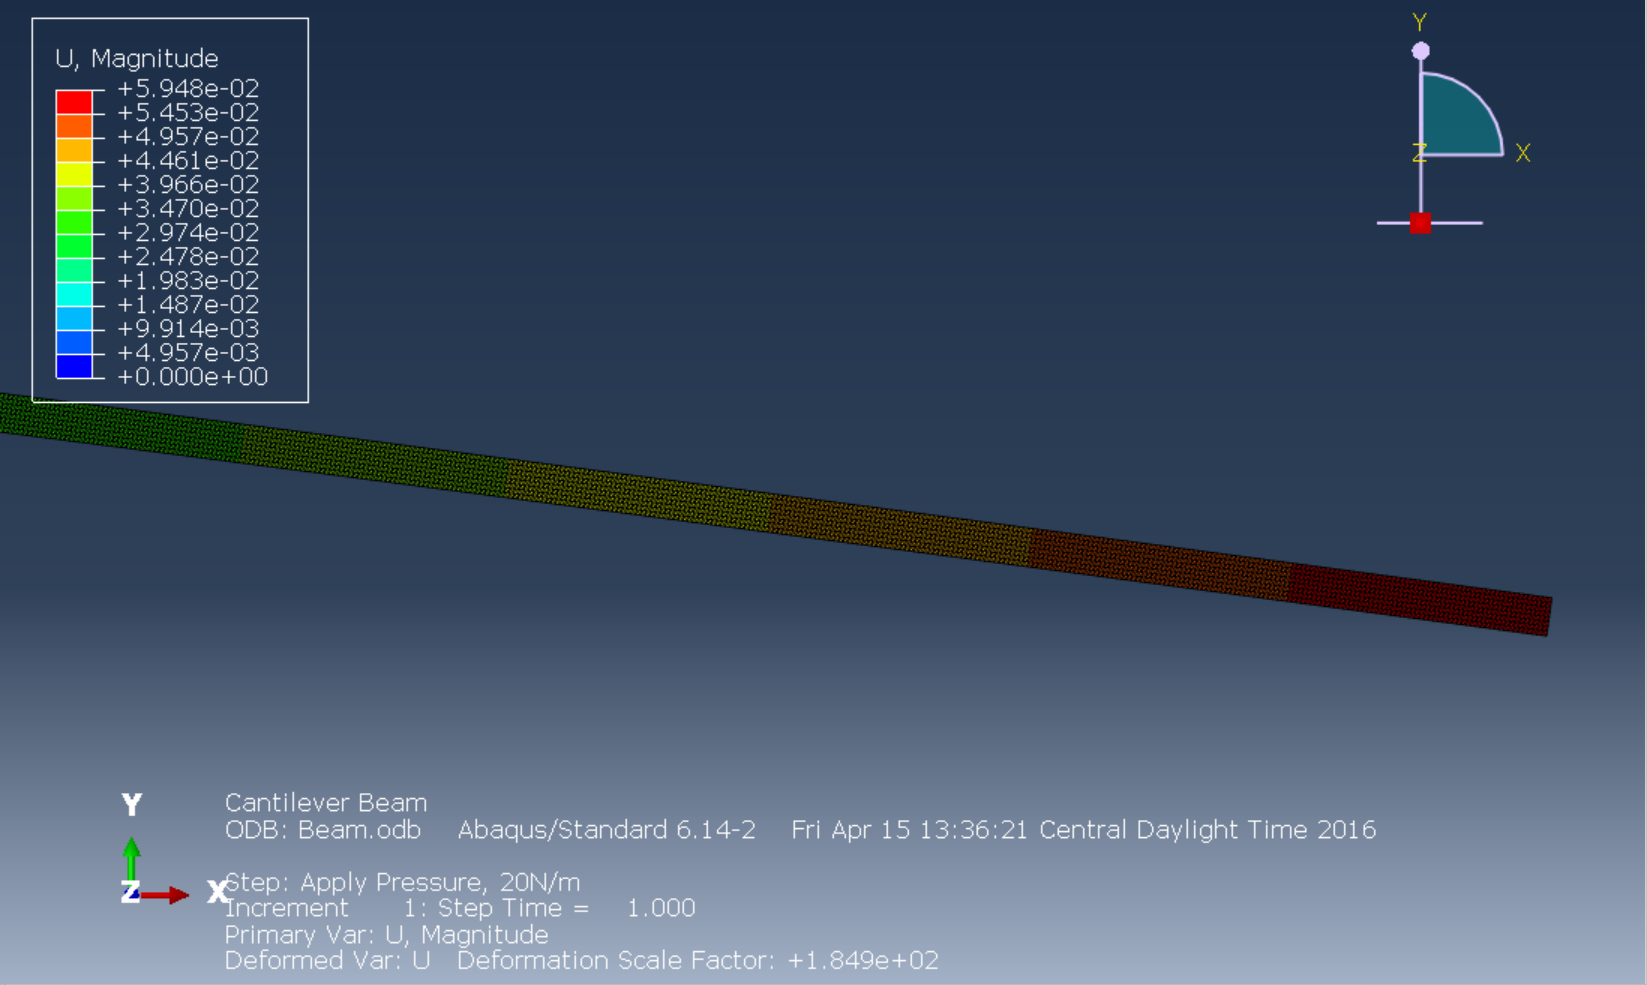
\includegraphics[scale=.50]{3Nsize0_125MDisplacement.PNG}
\caption{Deflection Contour, Element Size: 0.125, Number of Nodes: 7929, Number of Elements: 14,080, Maximum Deflection: 5.948 cm}
\end{figure}

\clearpage

\begin{figure}[ht]
\centering
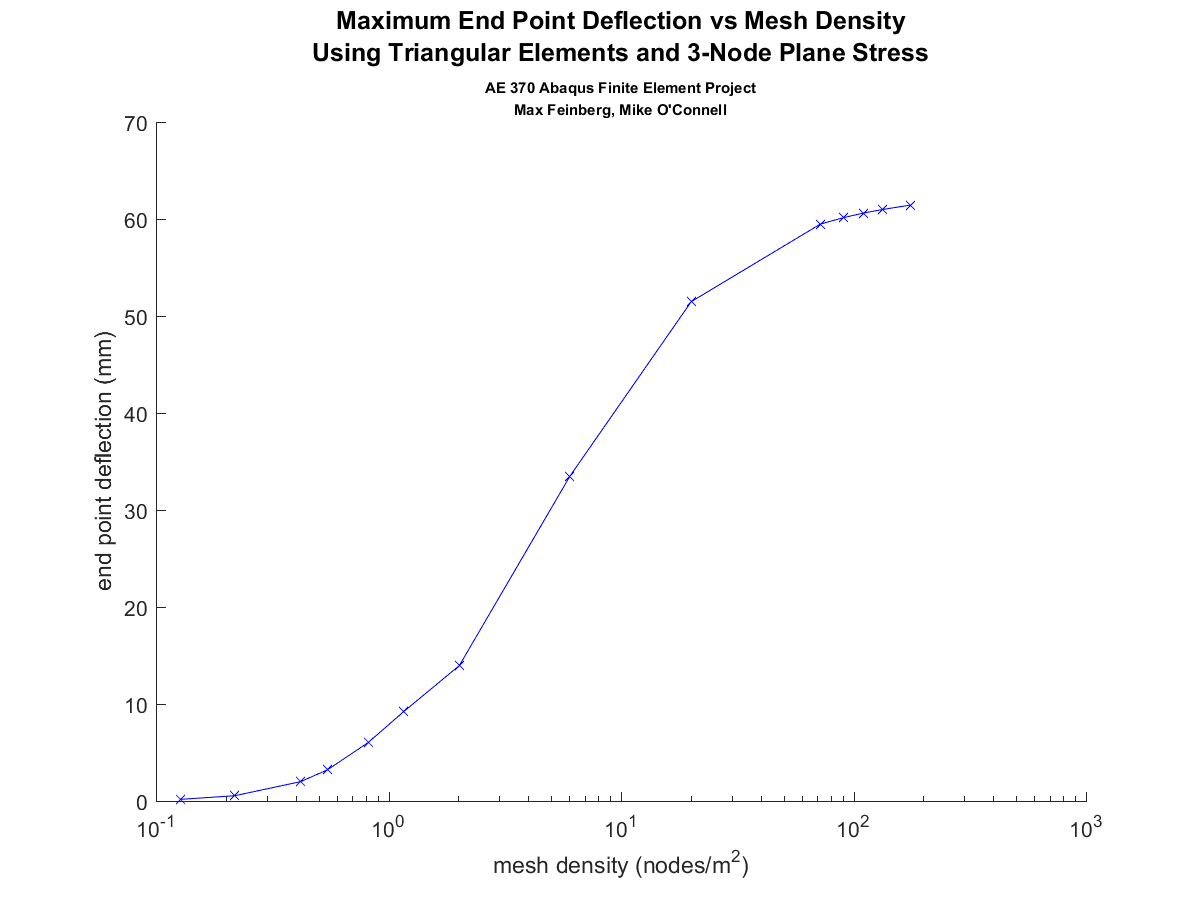
\includegraphics[scale=.55]{ae370abaqus_3node.png}
\caption{A Plot Showing the Convergence of the Maximum Deflection}
\end{figure}
Figure 22 above shows how the maximum deflection of the beam converges as the mesh density of the FEA model increases. Mesh density was calculated by dividing the number of nodes by the area of the beam. The simulations converge to a deflection of roughly 60 mm.  As it can be clearly seen in the plot, the change in end point deflection quickly decreases after the mesh density surpasses a value of roughly 100 $\frac{nodes}{m^{2}}$.\\

Convergence was confirmed by estimating the logarithmic derivative of the end point deflection as a function of element size. This was then scaled by the element size to account for the changes in element size step.  Once this value, which is referred to as the convergence value, was was sufficiently low, the solution was said to have converged close to the exact solution.  The convergence value is an estimate of the condition number of the end point deflection.  Thus, a low convergence value indicates that increasing mesh density will not substantially increase the end point deflection.
$$
ConvergenceValue = \frac{(ElementSize) \cdot (\Delta Deflection(ElementsSize))}{(\Delta ElementsSize) \cdot (Deflection(ElementSize))}
$$
Using 3-node plane stress elements and 12,111 nodes (110.1$\frac{nodes}{m^{2}}$), a convergence value of 0.0437 was reached, suggesting that the result is close to the exact solution.\\

\textbf{b)}
The problem was then analyzed using 6-node plane stress triangular elements. Figure 23 through Figure 42 show the stress and deflection contours.

\begin{figure}[ht]
\centering
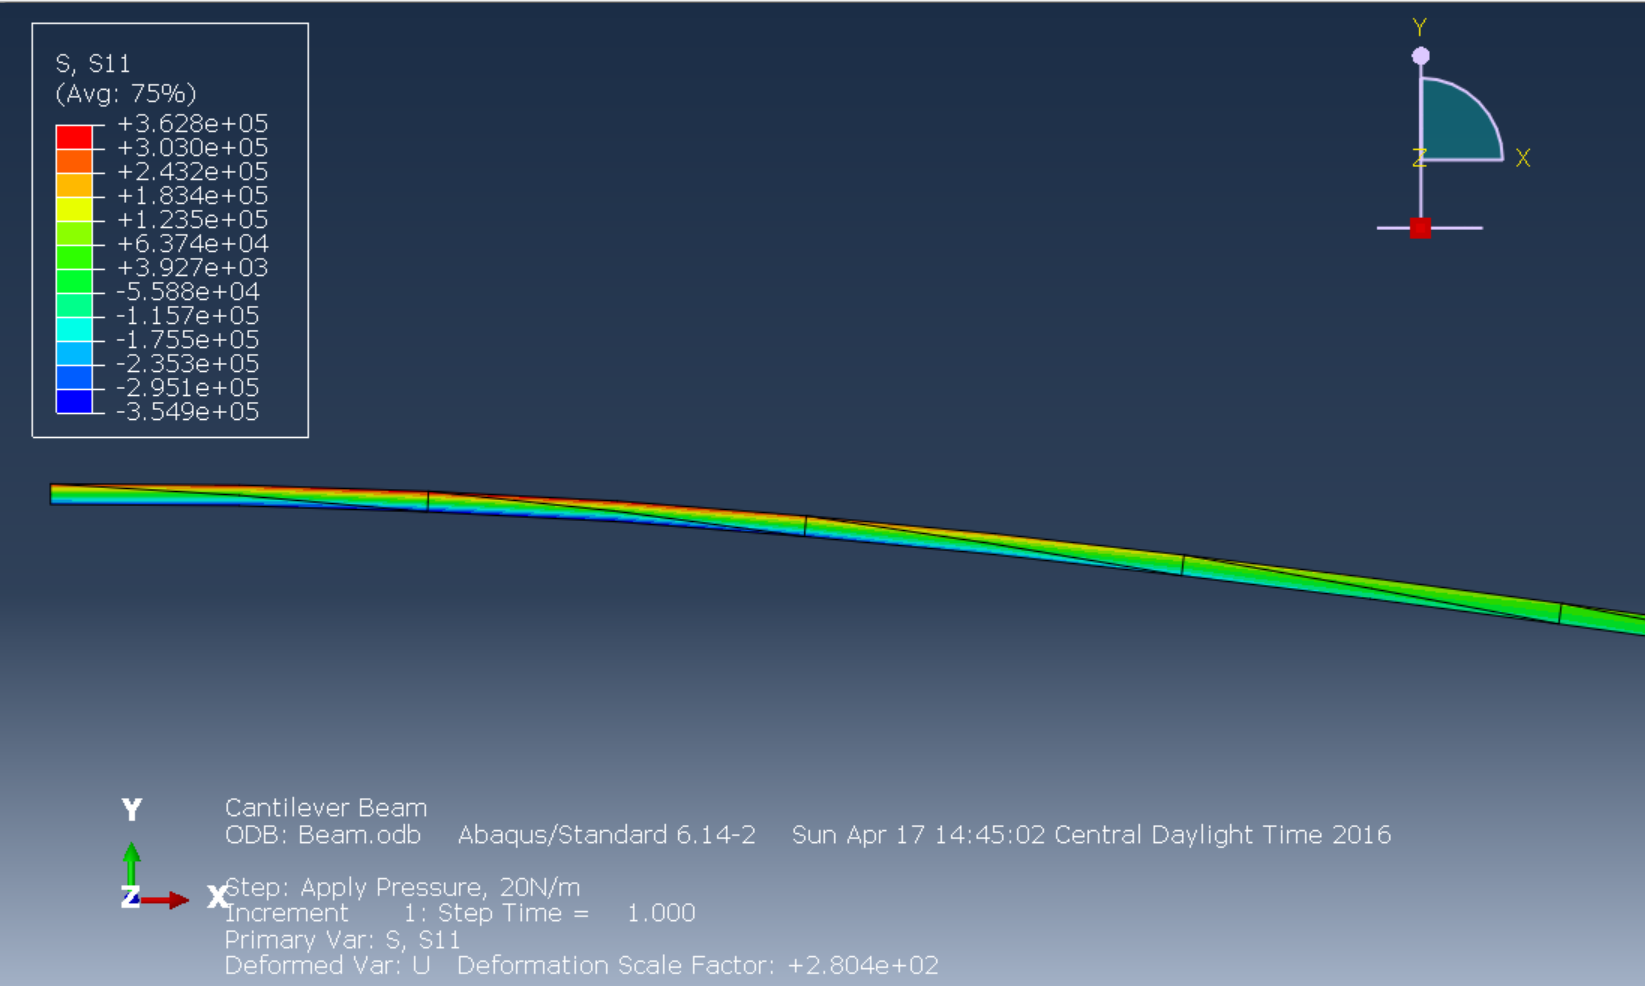
\includegraphics[scale=.5]{6Nsize20Stress.PNG}
\caption{Stress Contour, Element Size: 20, Number of Nodes: 39, Number of Elements: 12}
\end{figure}
\begin{figure}[ht]
\centering
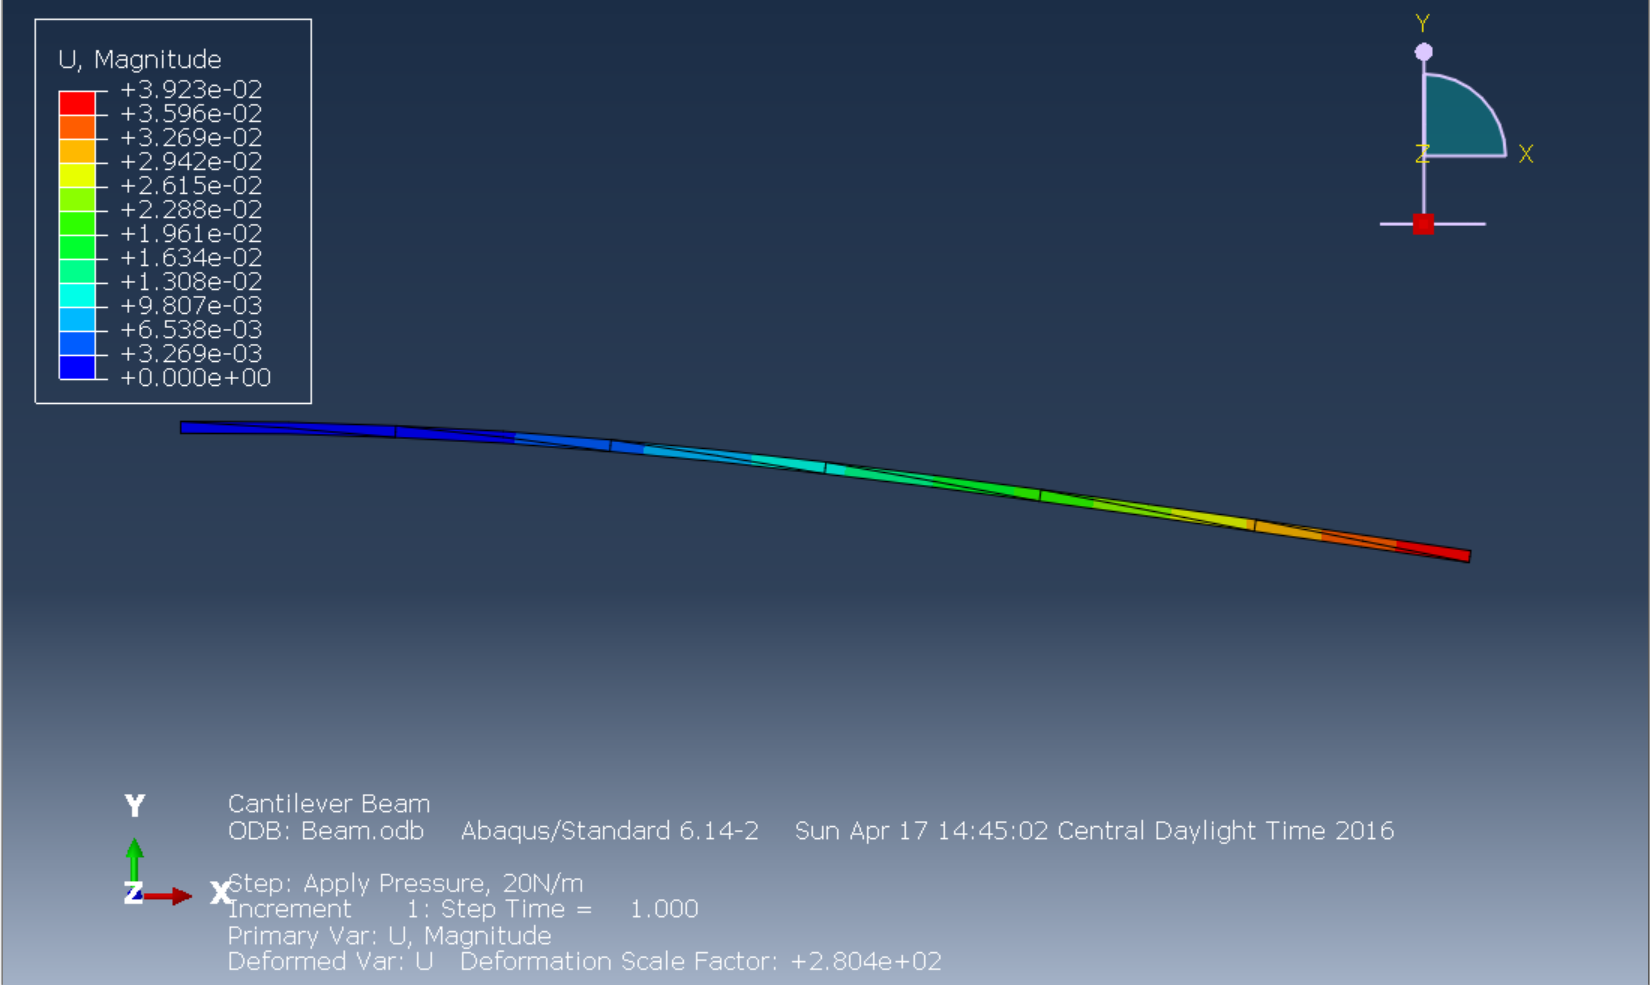
\includegraphics[scale=.5]{6Nsize20MDisplacement.PNG}
\caption{Deflection Contour, Element Size: 20, Number of Nodes: 39, Number of Elements: 12, Maximum Deflection: 3.923 cm}
\end{figure}

\begin{figure}[ht]
\centering
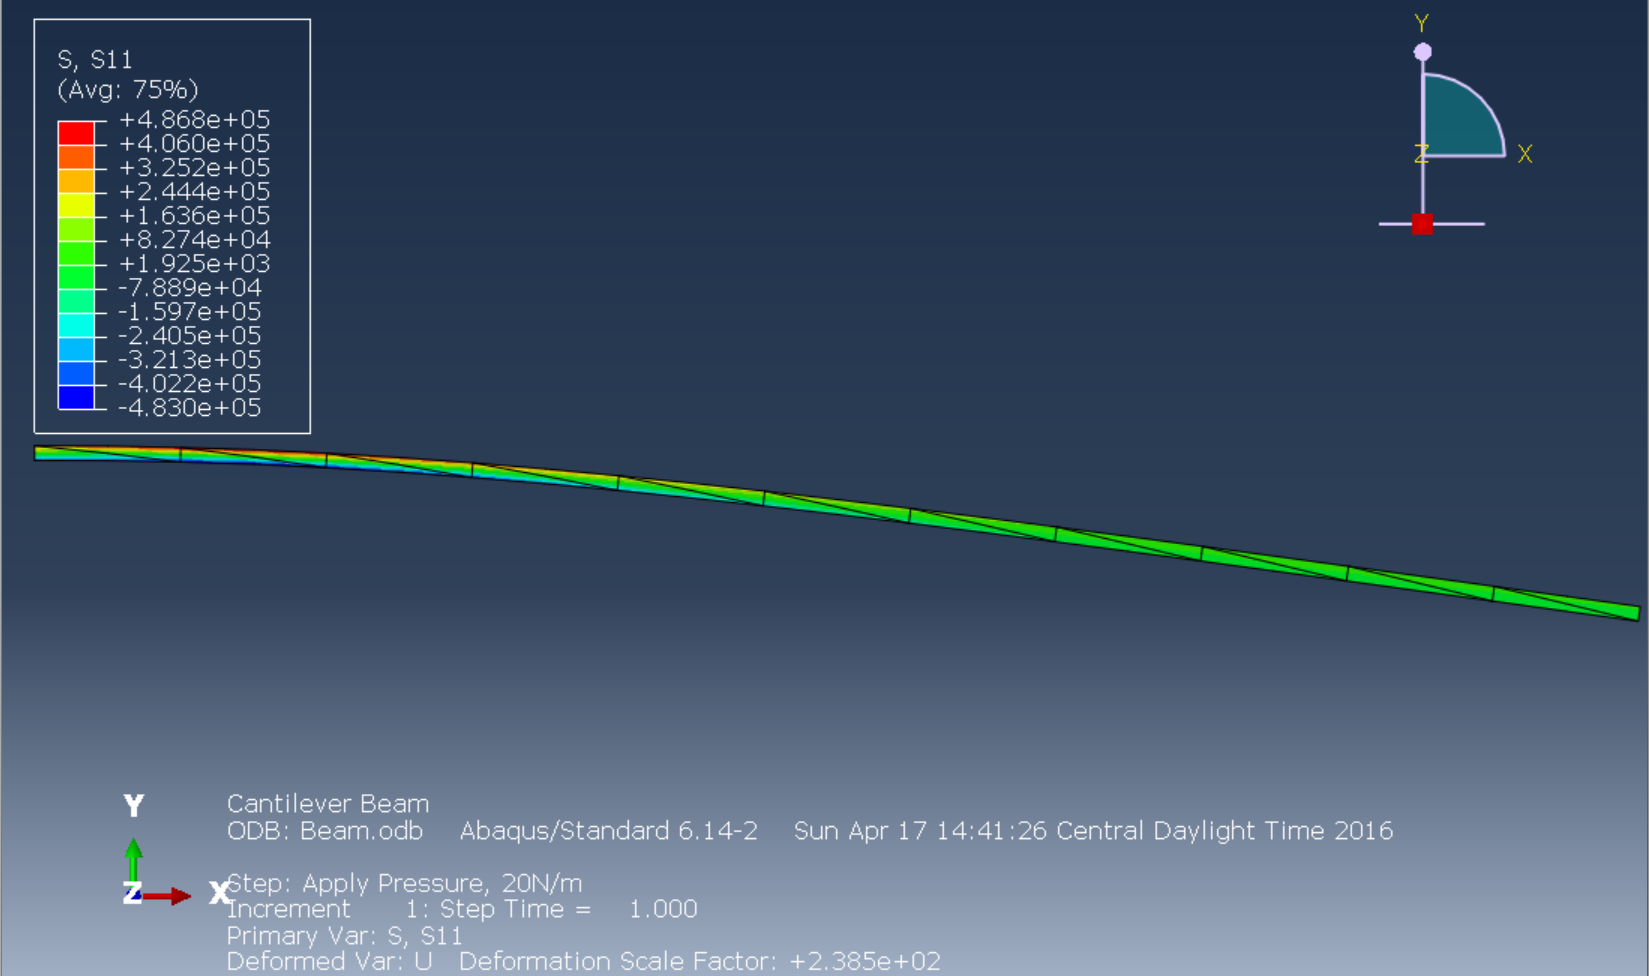
\includegraphics[scale=.5]{6Nsize10Stress.PNG}
\caption{Stress Contour, Element Size: 10, Number of Nodes: 69, Number of Elements: 22}
\end{figure}
\begin{figure}[ht]
\centering
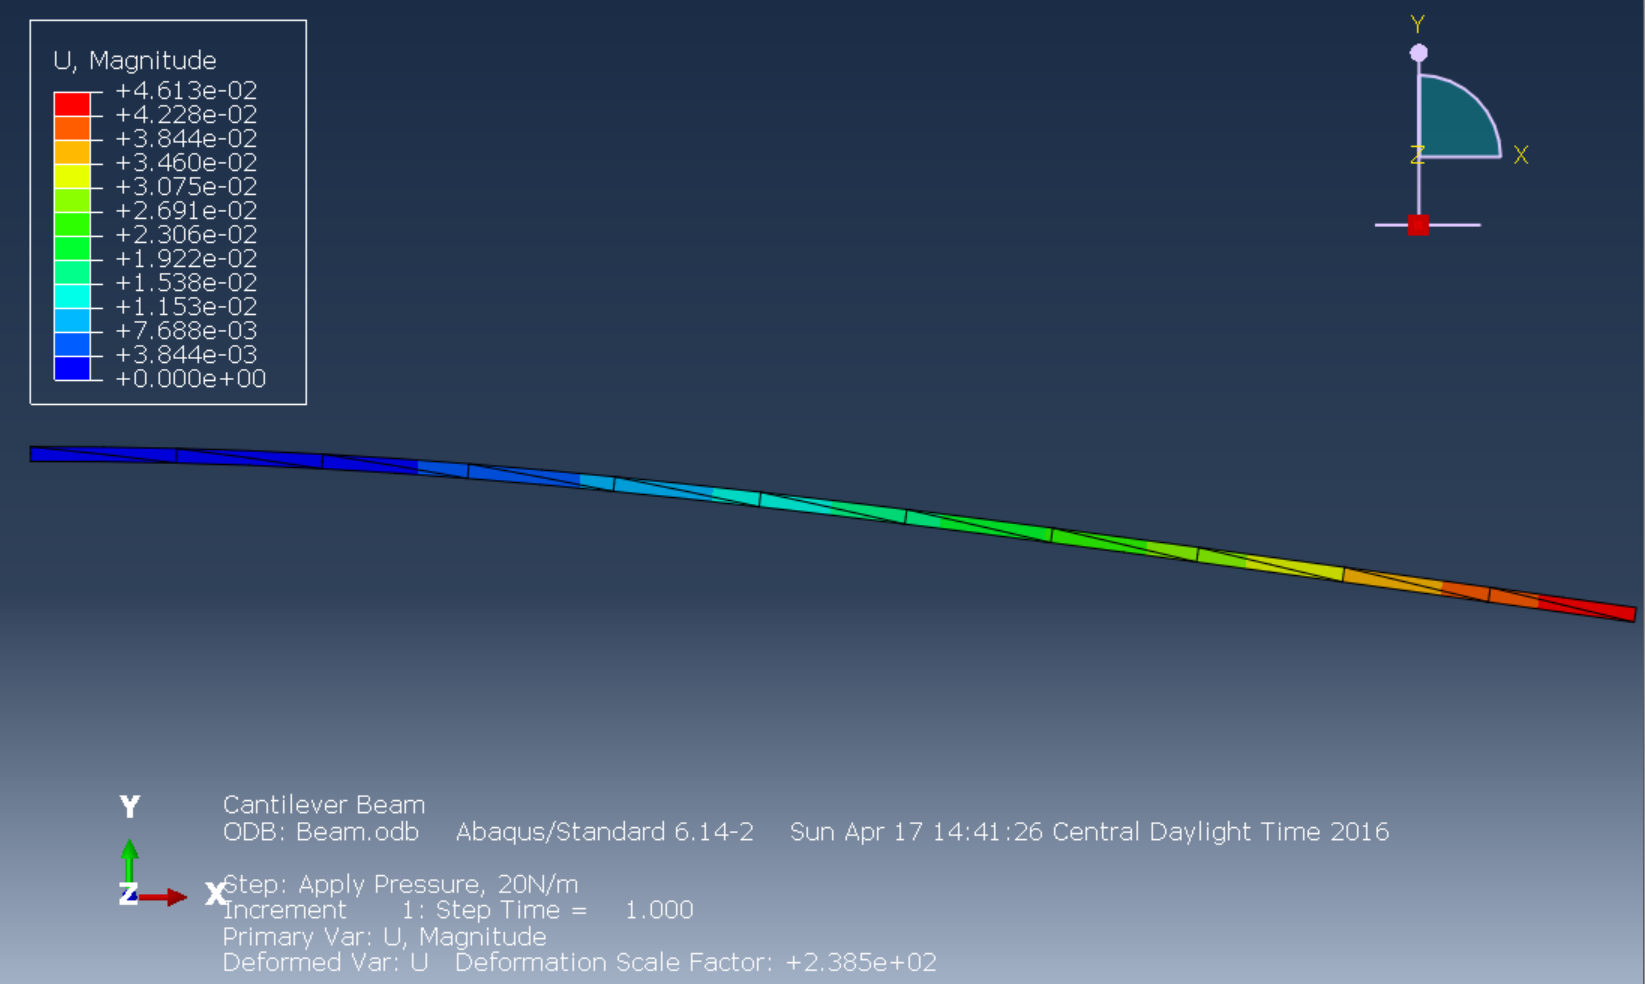
\includegraphics[scale=.5]{6Nsize10MDisplacement.PNG}
\caption{Deflection Contour, Element Size: 10, Number of Nodes: 69, Number of Elements: 22, Maximum Deflection: 4.613 cm}
\end{figure}

\begin{figure}[ht]
\centering
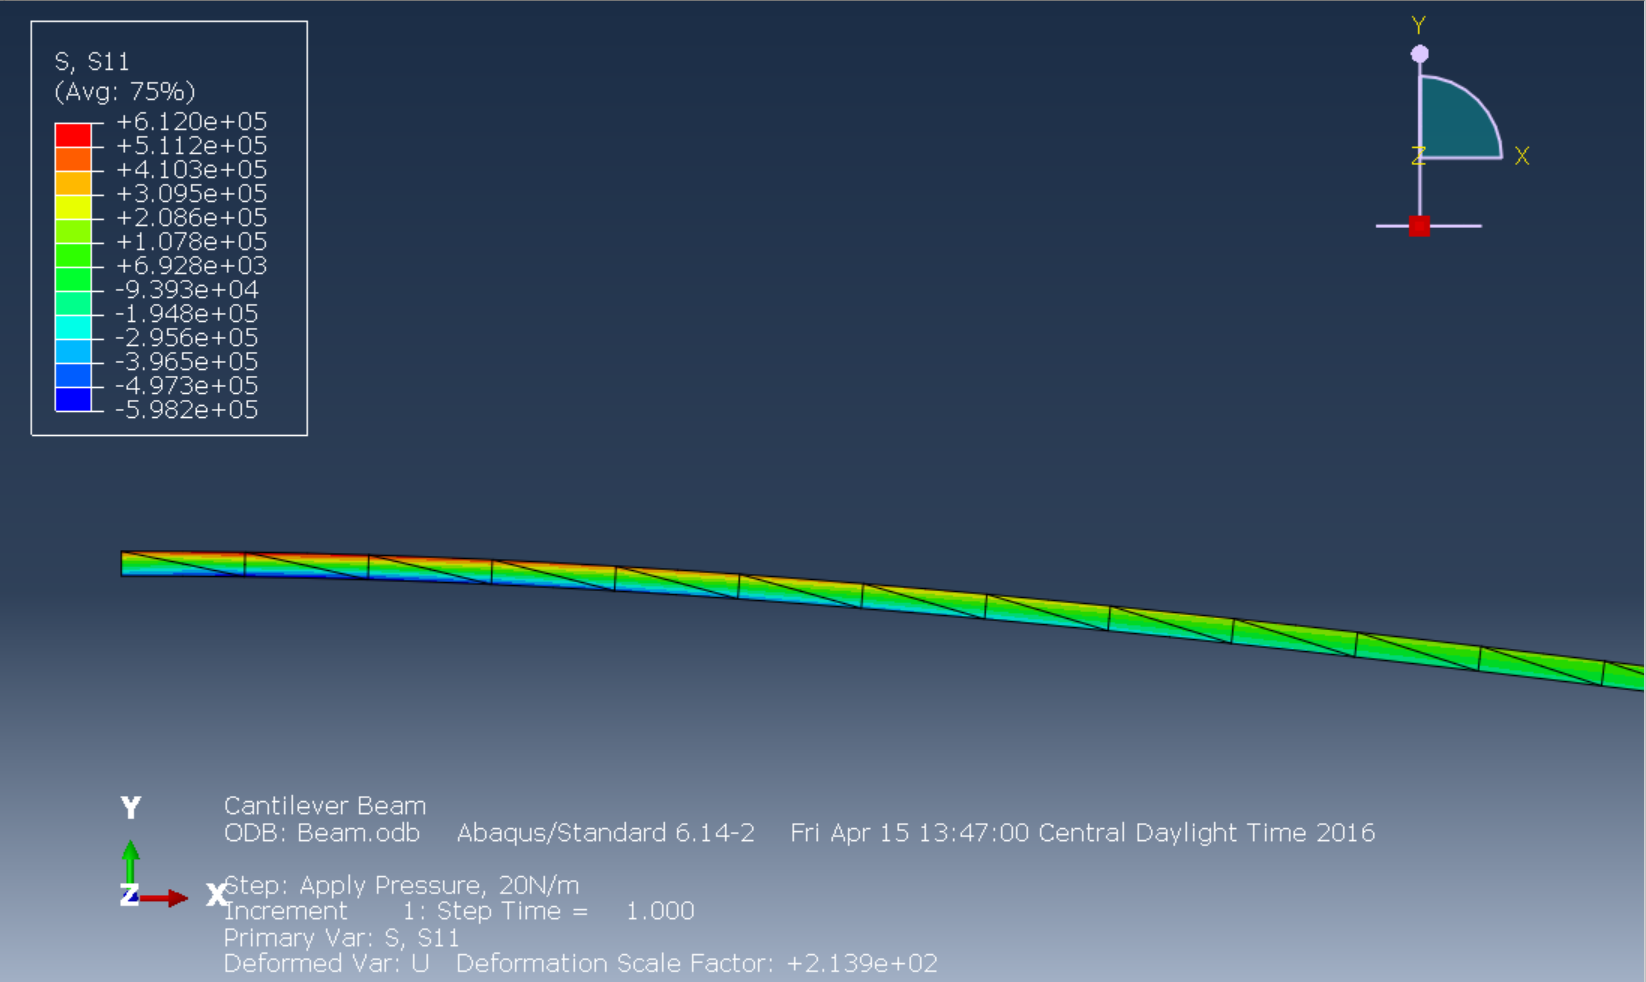
\includegraphics[scale=.5]{6Nsize5Stress.PNG}
\caption{Stress Contour, Element Size: 5, Number of Nodes: 135, Number of Elements: 44}
\end{figure}
\begin{figure}[ht]
\centering
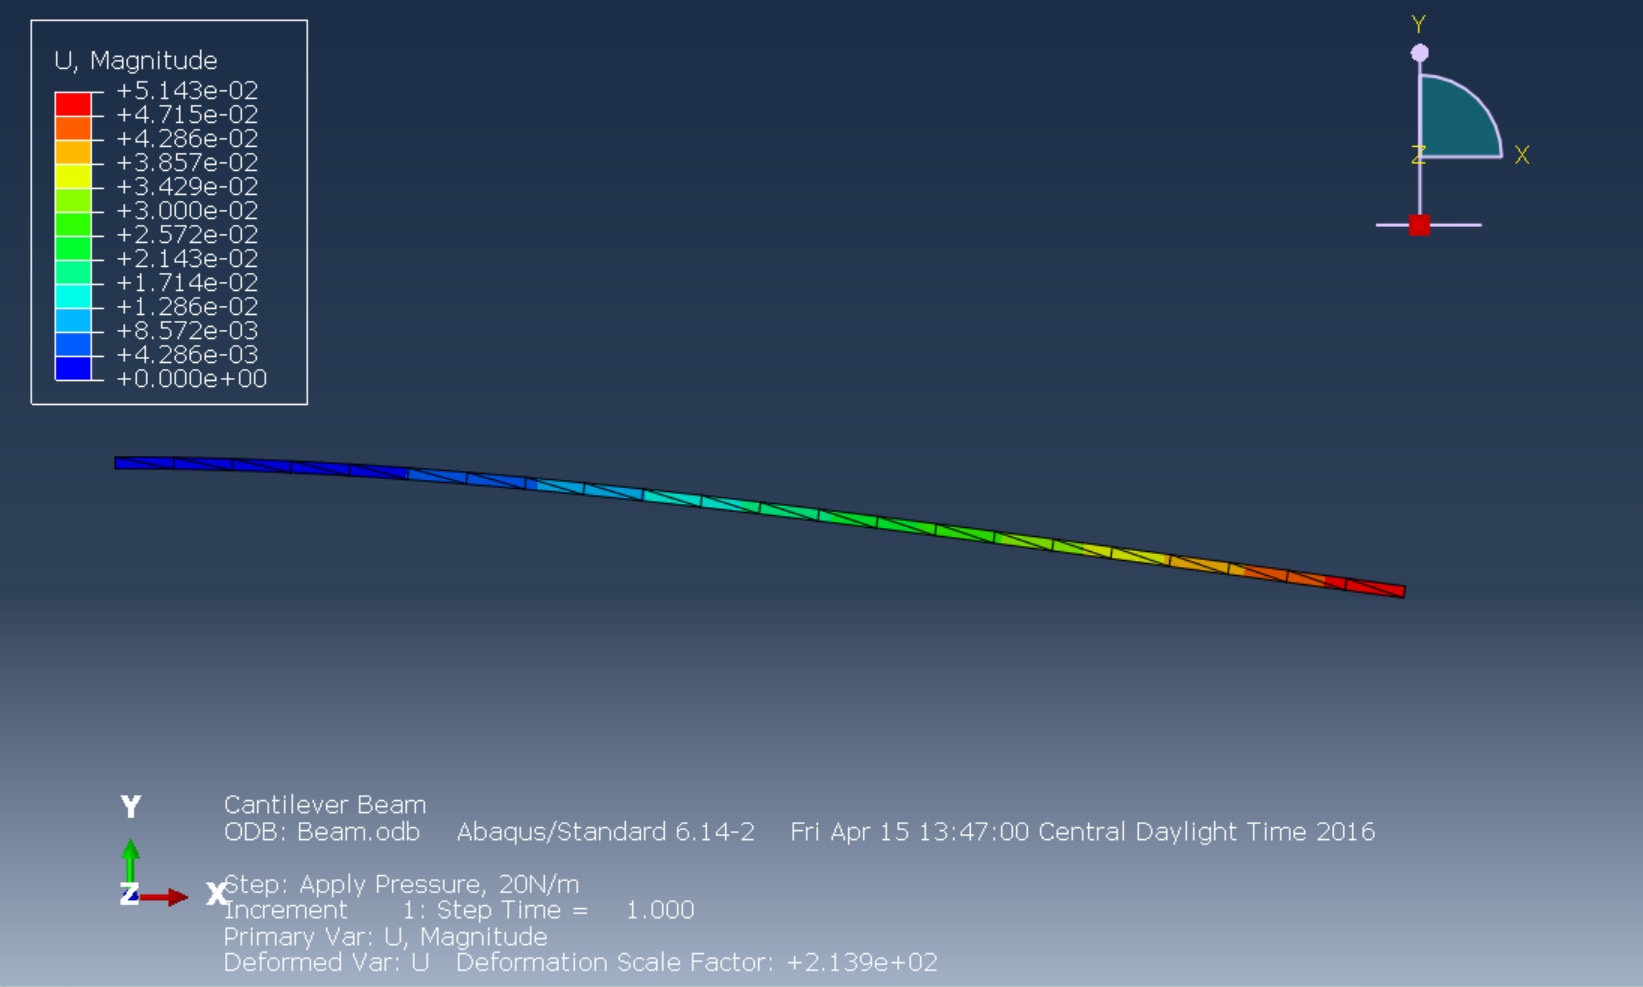
\includegraphics[scale=.5]{6Nsize5MDisplacement.PNG}
\caption{Deflection Contour, Element Size: 5, Number of Nodes: 135, Number of Elements: 44, Maximum Deflection: 5.143 cm}
\end{figure}

\begin{figure}[ht]
\centering
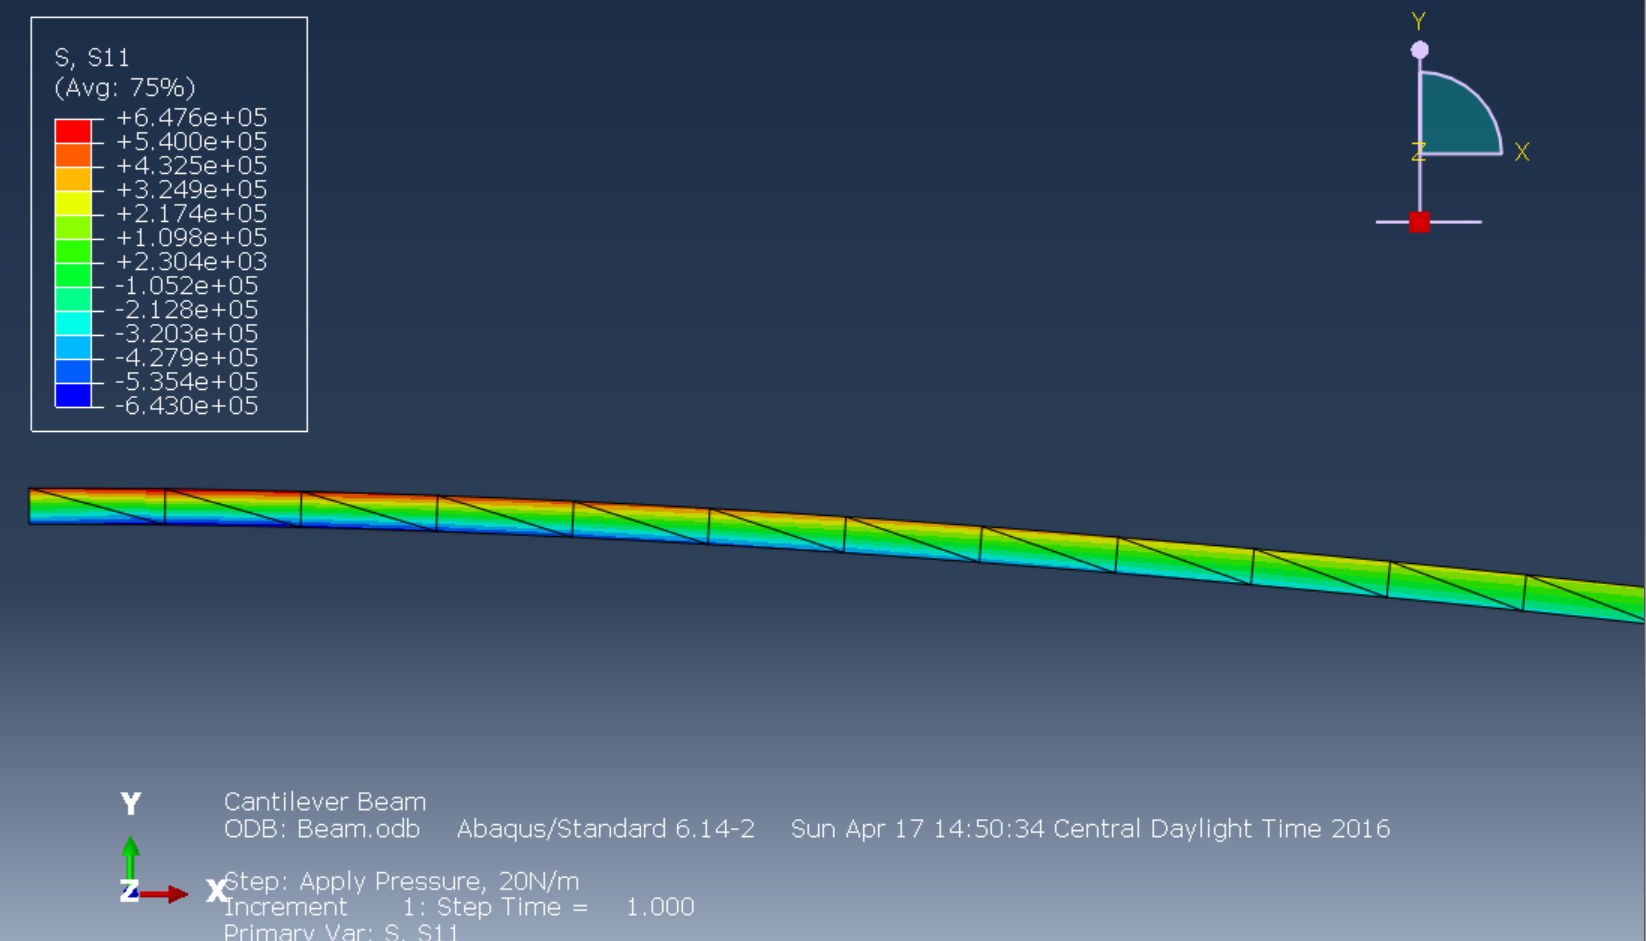
\includegraphics[scale=.5]{6Nsize3_75Stress.PNG}
\caption{Stress Contour, Element Size: 3.75, Number of Nodes: 177, Number of Elements: 58}
\end{figure}
\begin{figure}[ht]
\centering
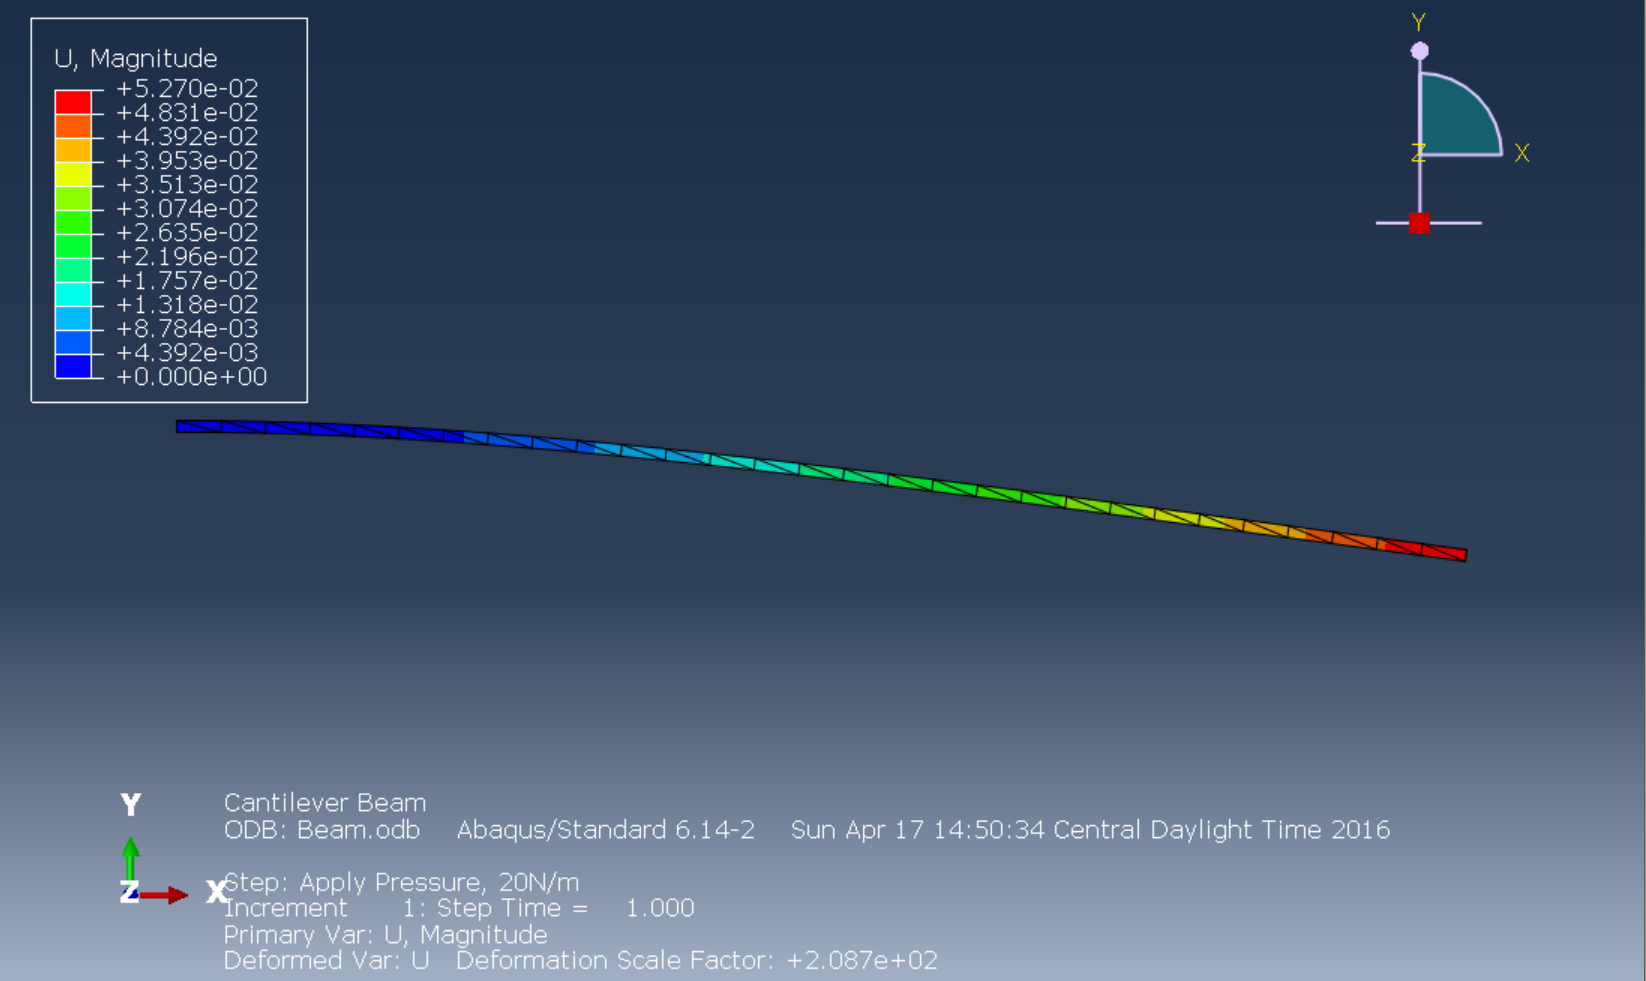
\includegraphics[scale=.5]{6Nsize3_75MDisplacement.PNG}
\caption{Deflection Contour, Element Size: 3.75, Number of Nodes: 177, Number of Elements: 58, Maximum Deflection 5.270 cm}
\end{figure}

\begin{figure}[ht]
\centering
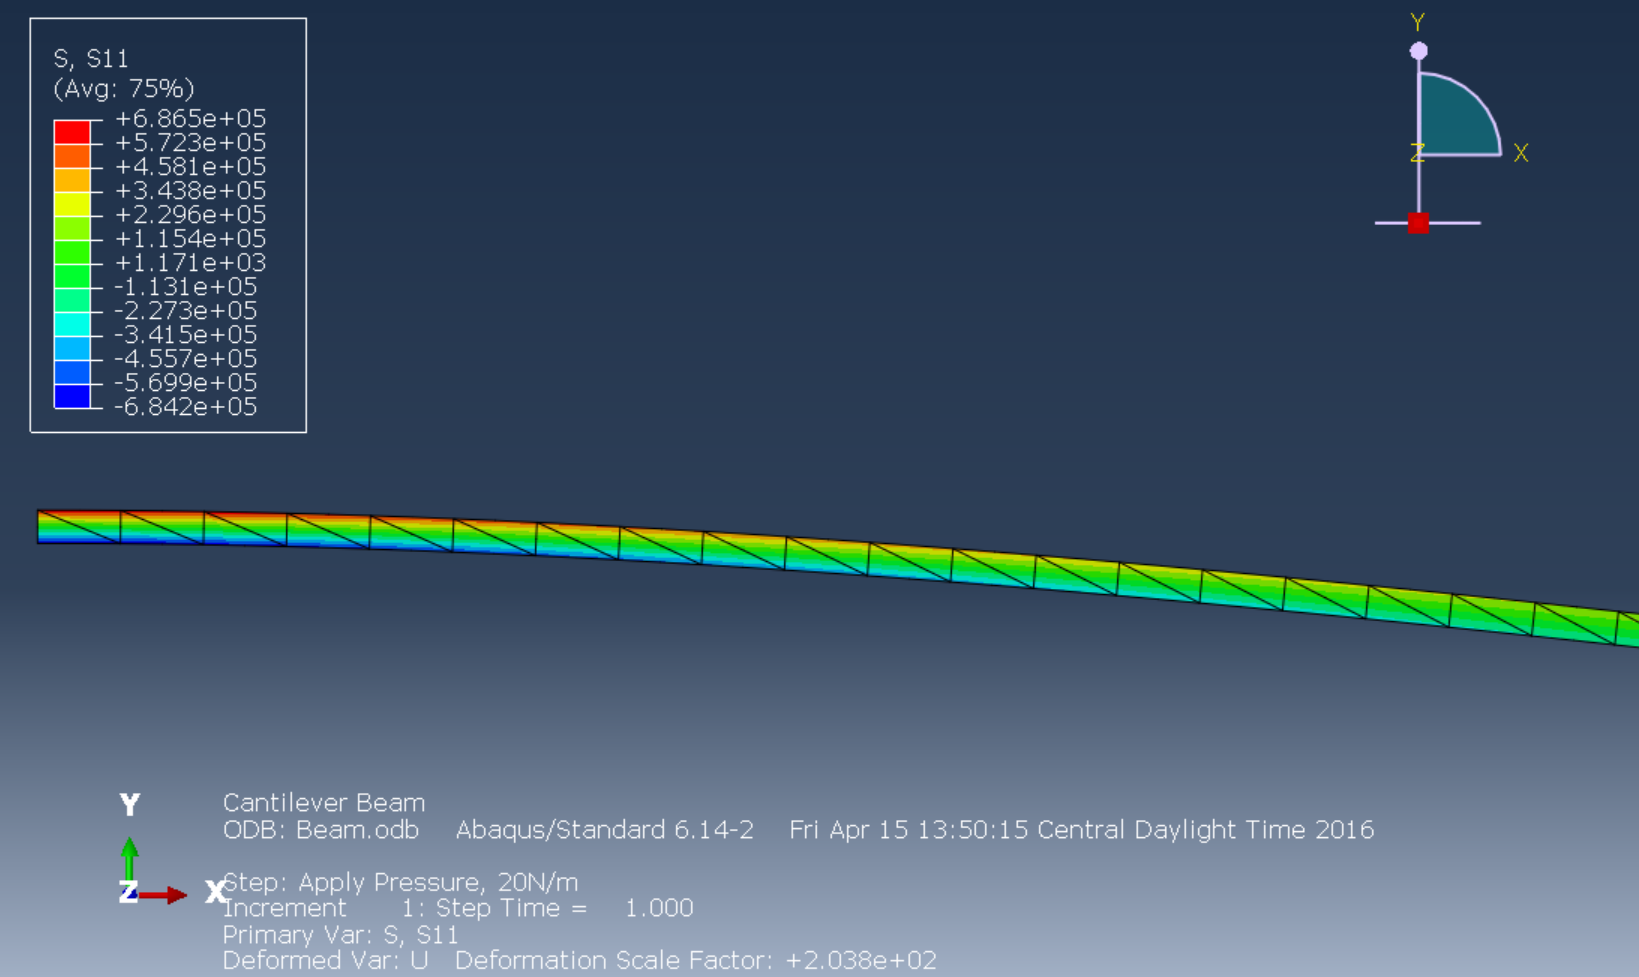
\includegraphics[scale=.5]{6Nsize2_5Stress.PNG}
\caption{Stress Contour, Element Size: 2.5, Number of Nodes: 267, Number of Elements: 88}
\end{figure}
\begin{figure}[ht]
\centering
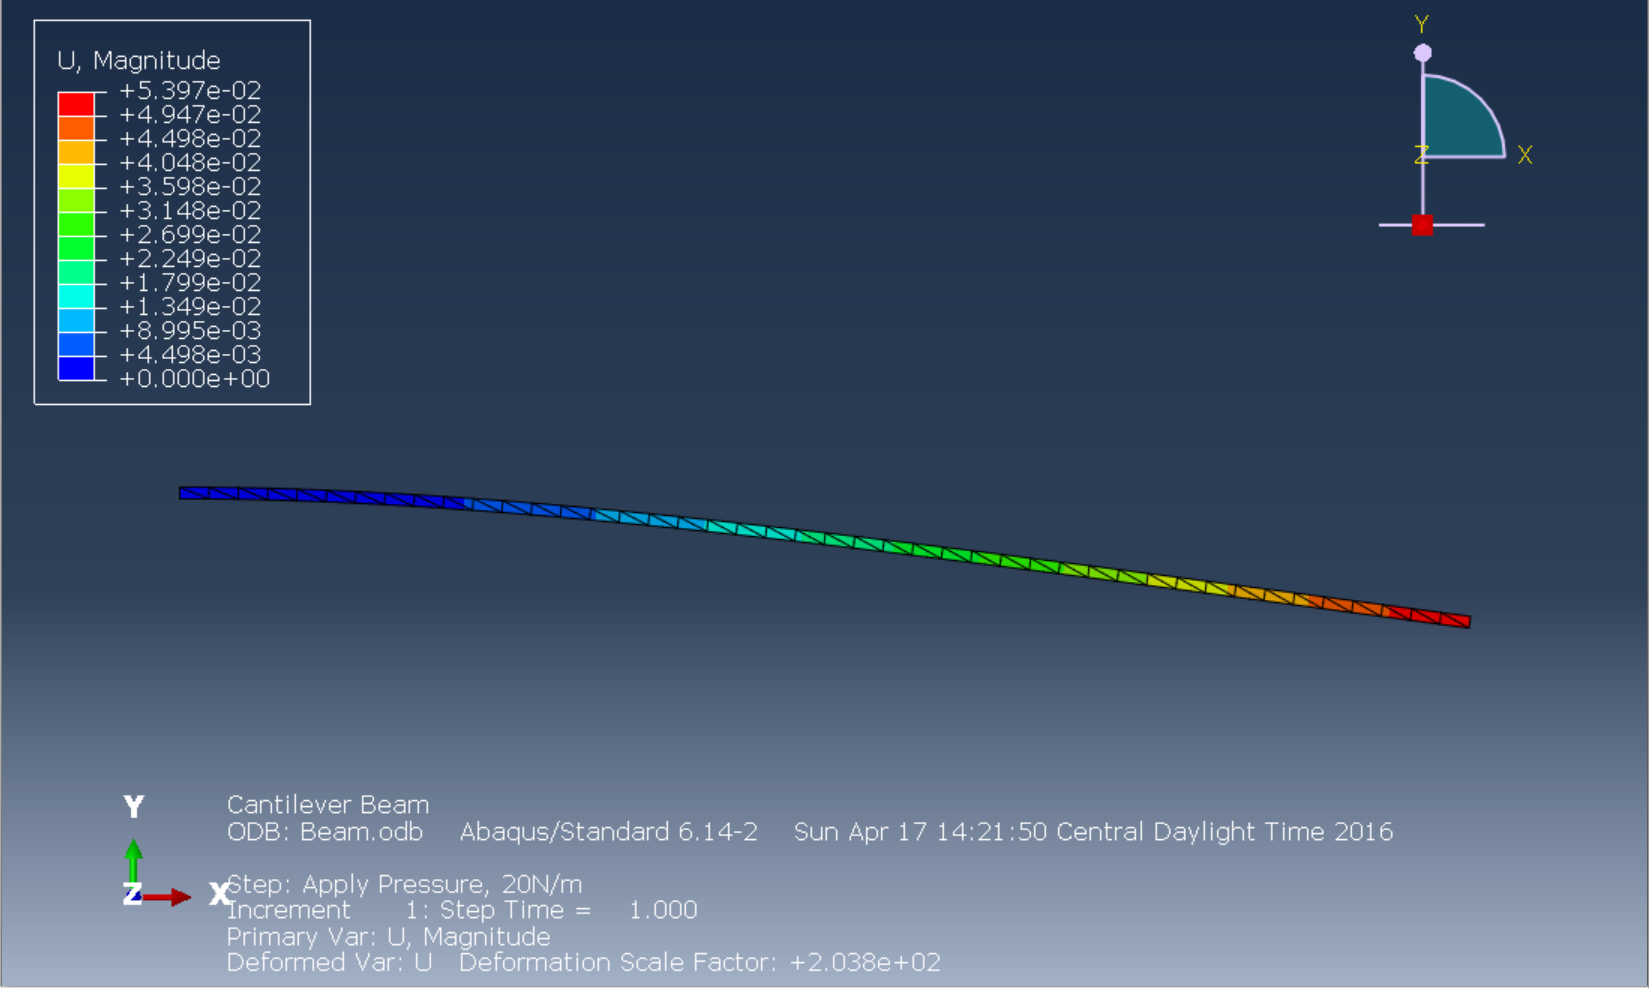
\includegraphics[scale=.5]{6Nsize2_5MDisplacement.PNG}
\caption{Deflection Contour, Element Size: 2.5, Number of Nodes: 267, Number of Elements: 88, Maximum Deflection: 5.397 cm}
\end{figure}

\begin{figure}[ht]
\centering
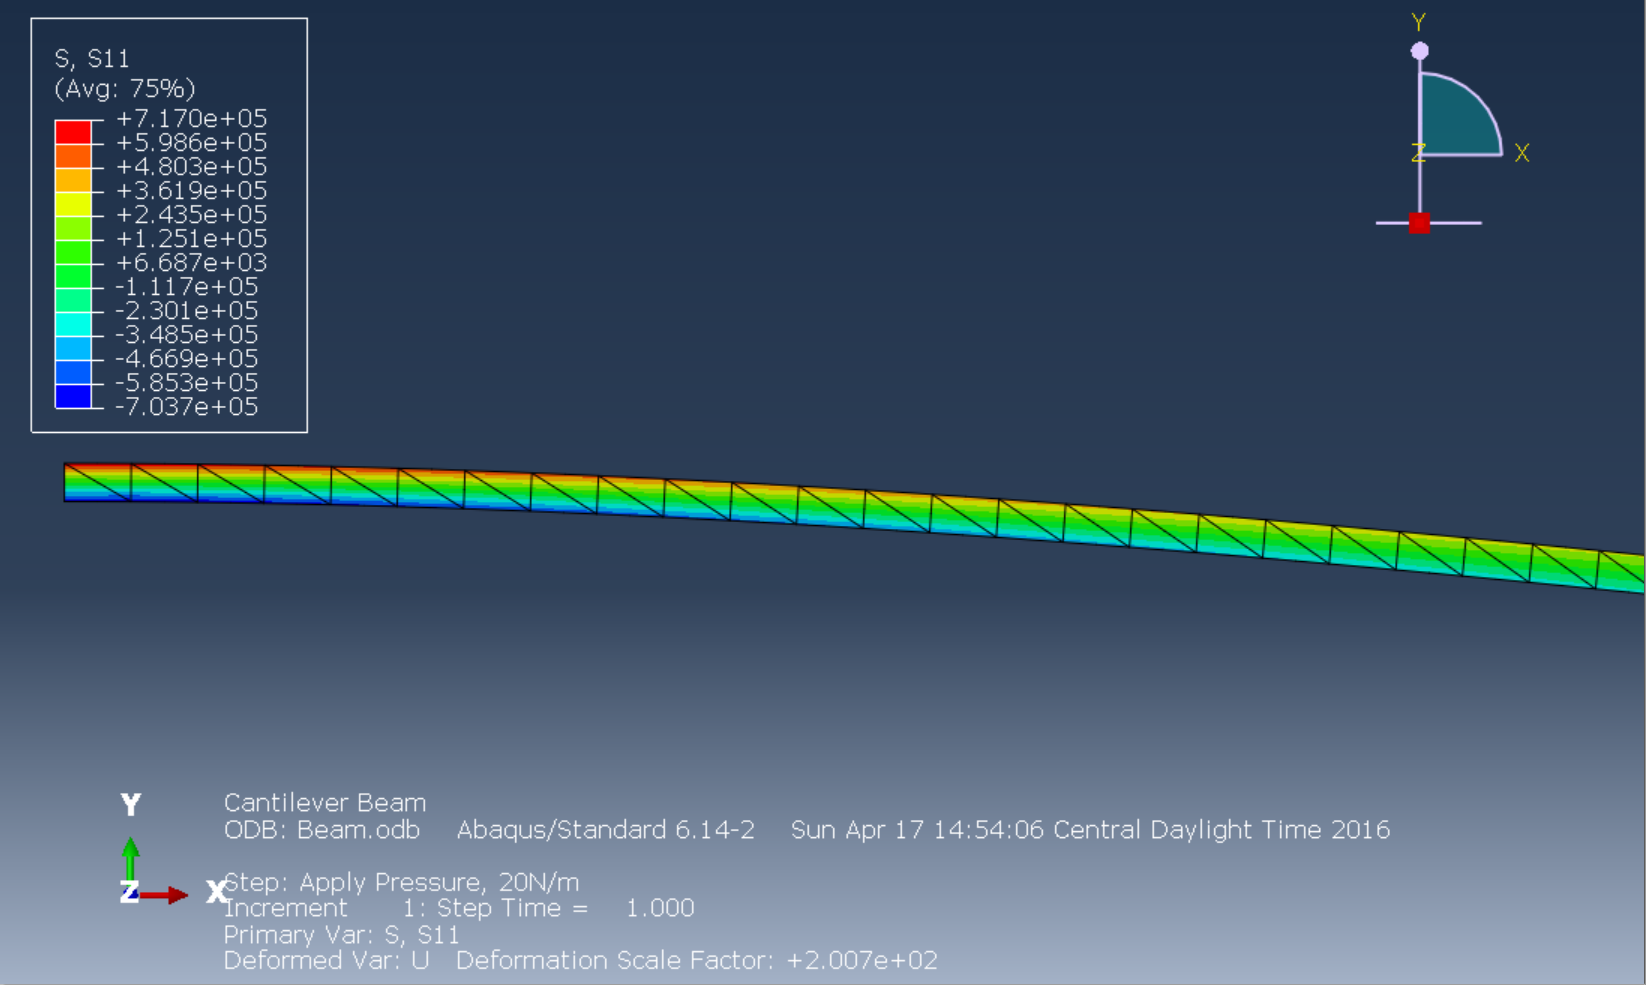
\includegraphics[scale=.5]{6Nsize1_75Stress.PNG}
\caption{Stress Contour, Element Size: 1.75, Number of Nodes: 381, Number of Elements: 126}
\end{figure}
\begin{figure}[ht]
\centering
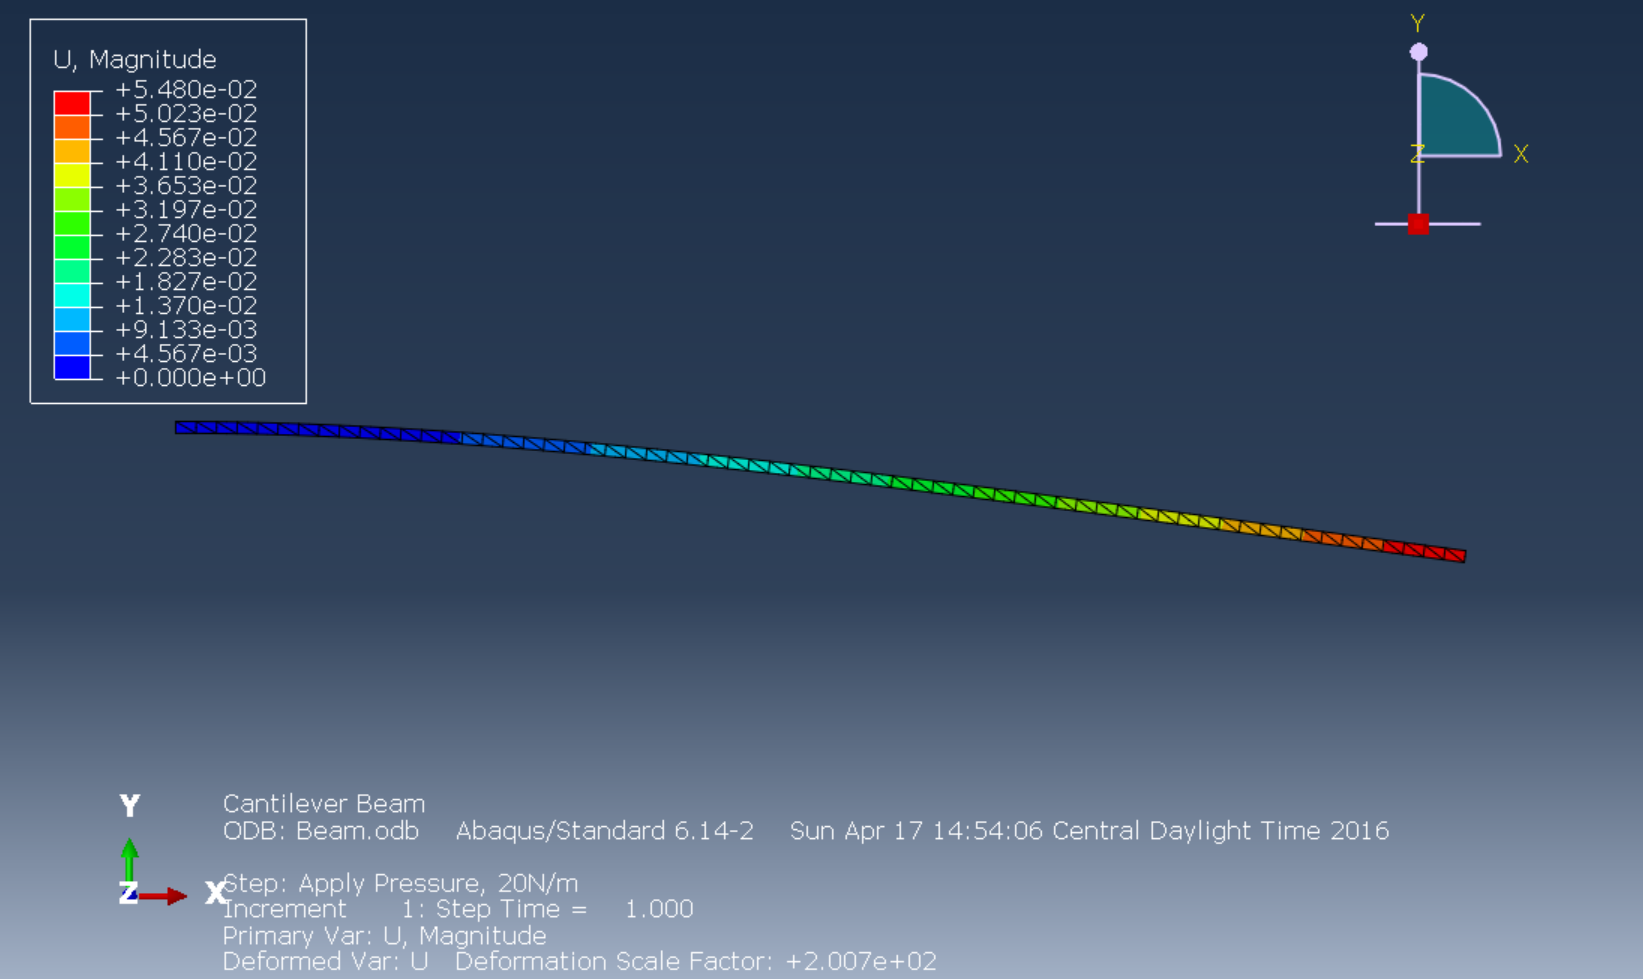
\includegraphics[scale=.5]{6Nsize1_75MDisplacement.PNG}
\caption{Deflection Contour, Element Size: 1.75, Number of Nodes: 381, Number of Elements: 126, Maximum Deflection 5.480 cm}
\end{figure}

\begin{figure}[ht]
\centering
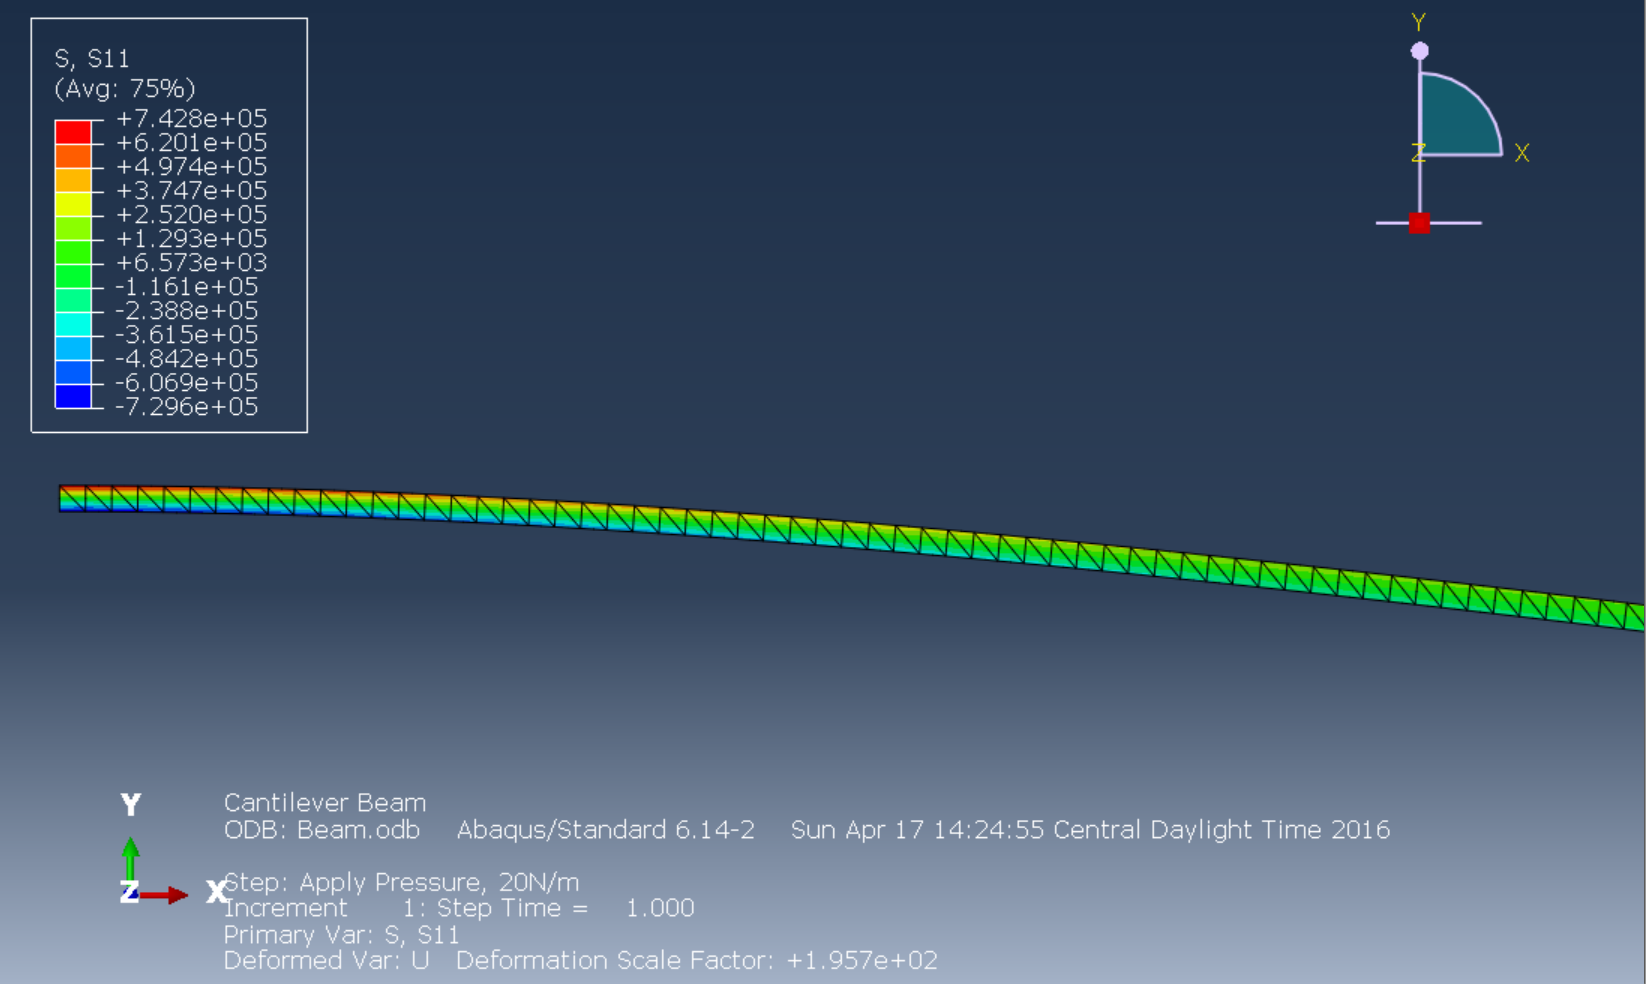
\includegraphics[scale=.5]{6Nsize1Stress.PNG}
\caption{Stress Contour, Element Size: 1, Number of Nodes: 663, Number of Elements: 220}
\end{figure}
\begin{figure}[ht]
\centering
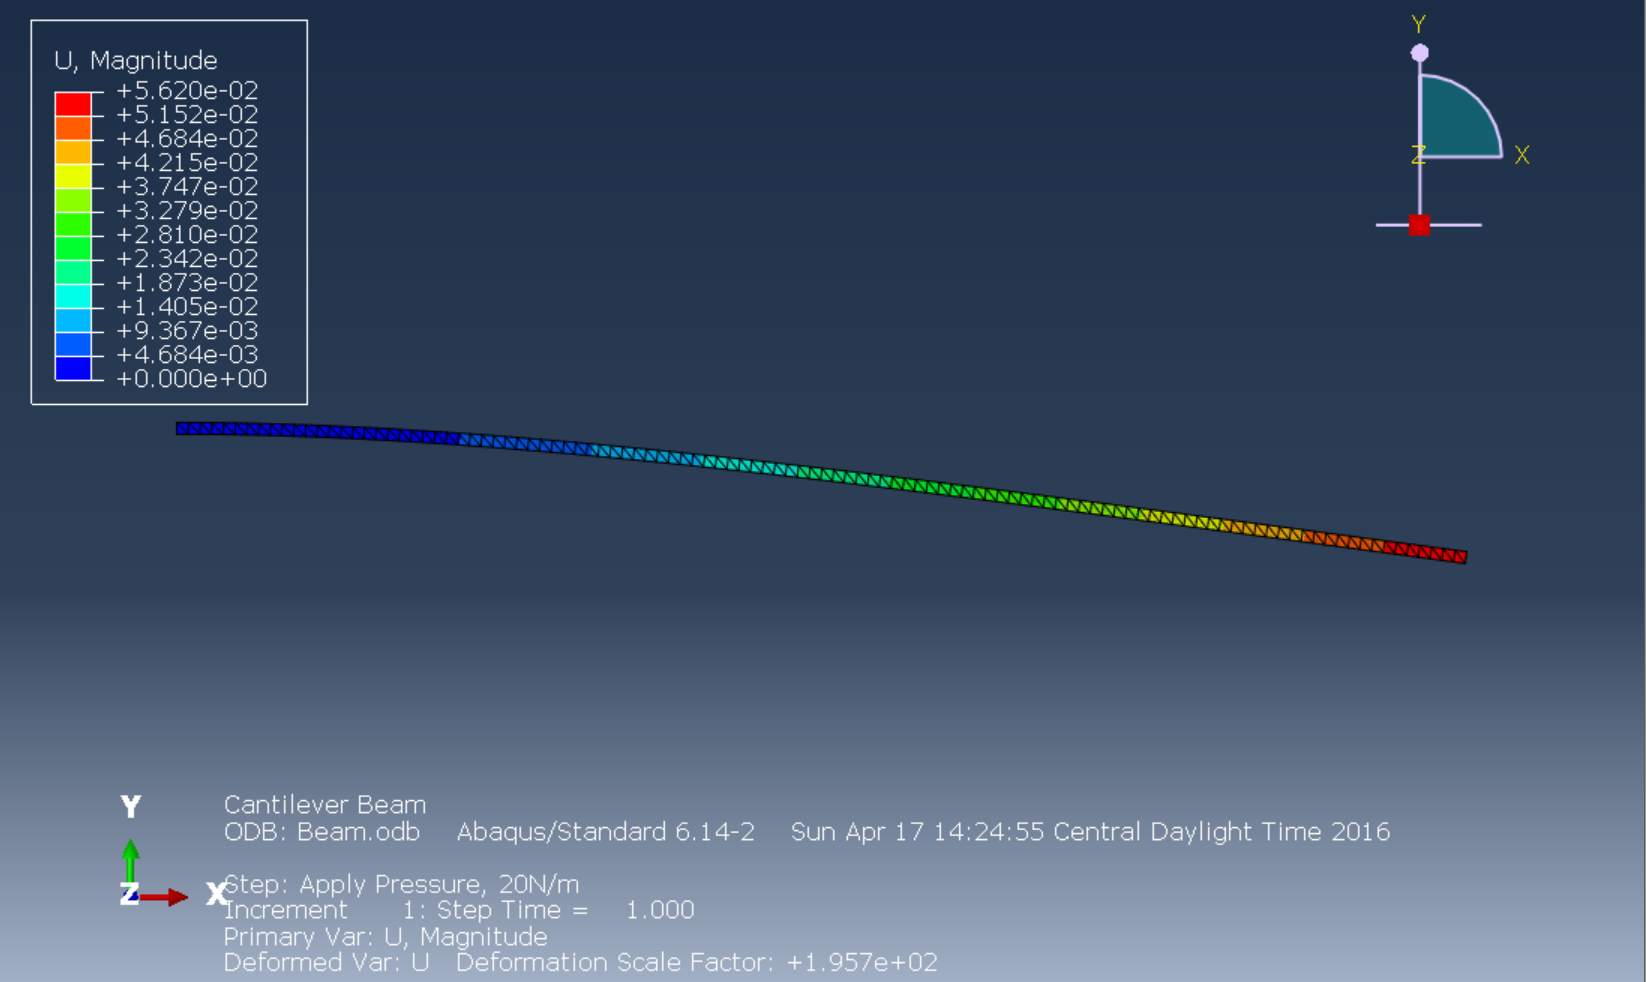
\includegraphics[scale=.5]{6Nsize1MDisplacement.PNG}
\caption{Deflection Contour, Element Size: 1, Number of Nodes: 663, Number of Elements: 220, Maximum Deflection: 5.620 cm}
\end{figure}

\begin{figure}[ht]
\centering
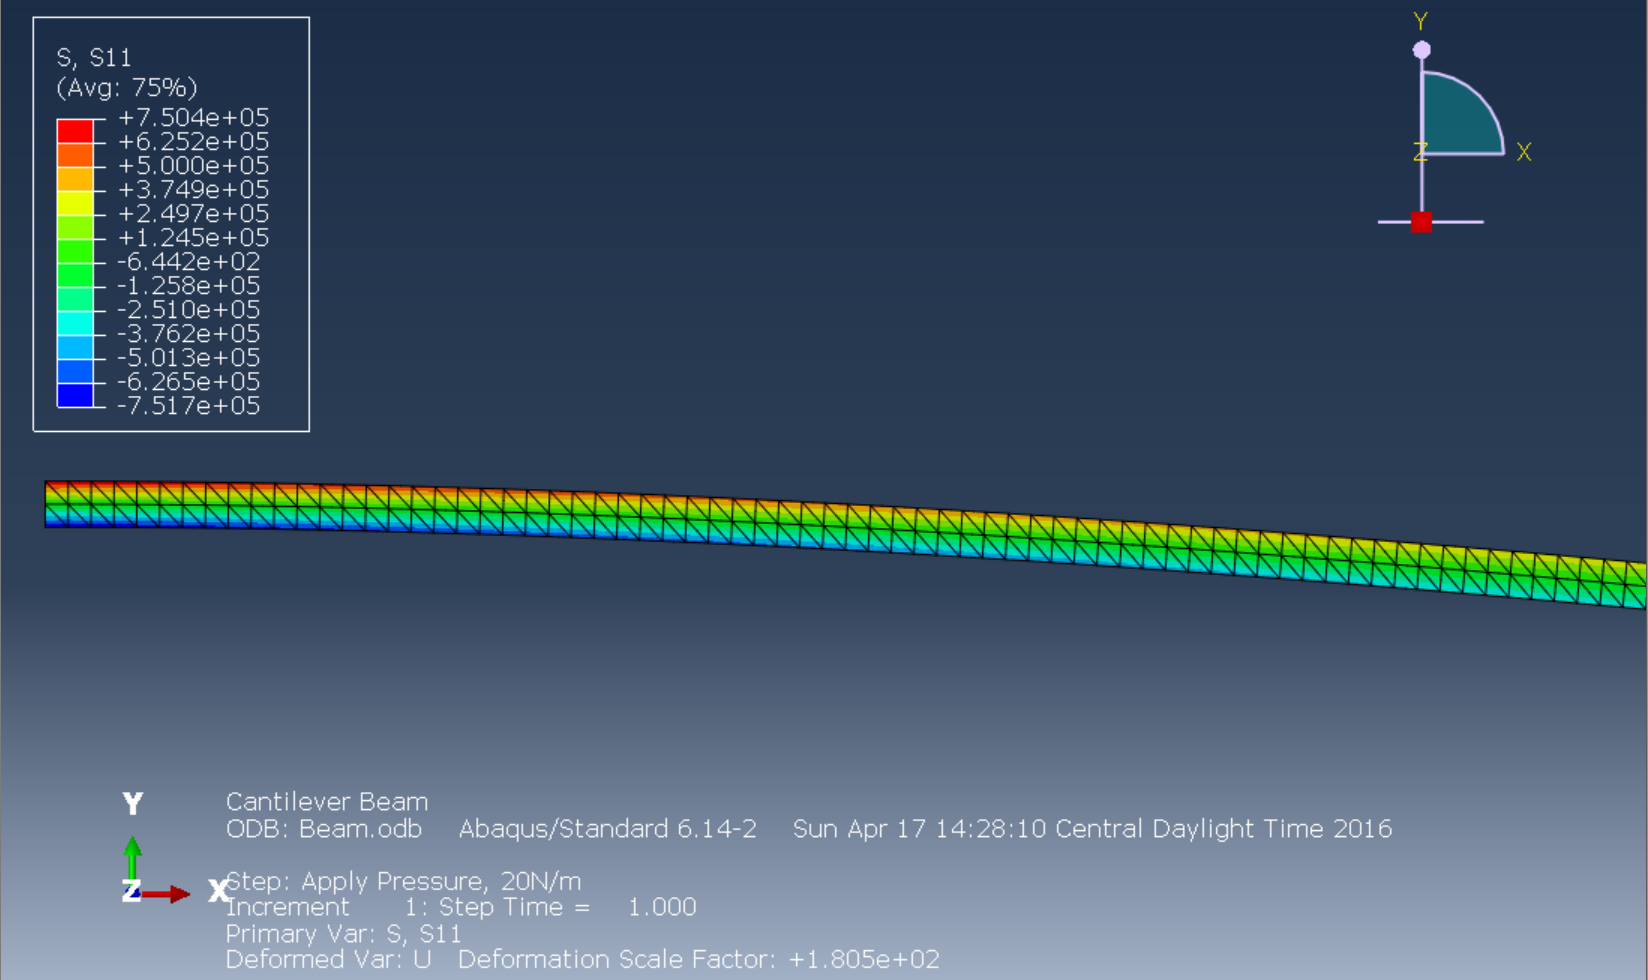
\includegraphics[scale=.5]{6Nsize0_5Stress.PNG}
\caption{Stress Contour, Element Size: 0.5, Number of Nodes: 2205, Number of Elements: 880}
\end{figure}
\begin{figure}[ht]
\centering
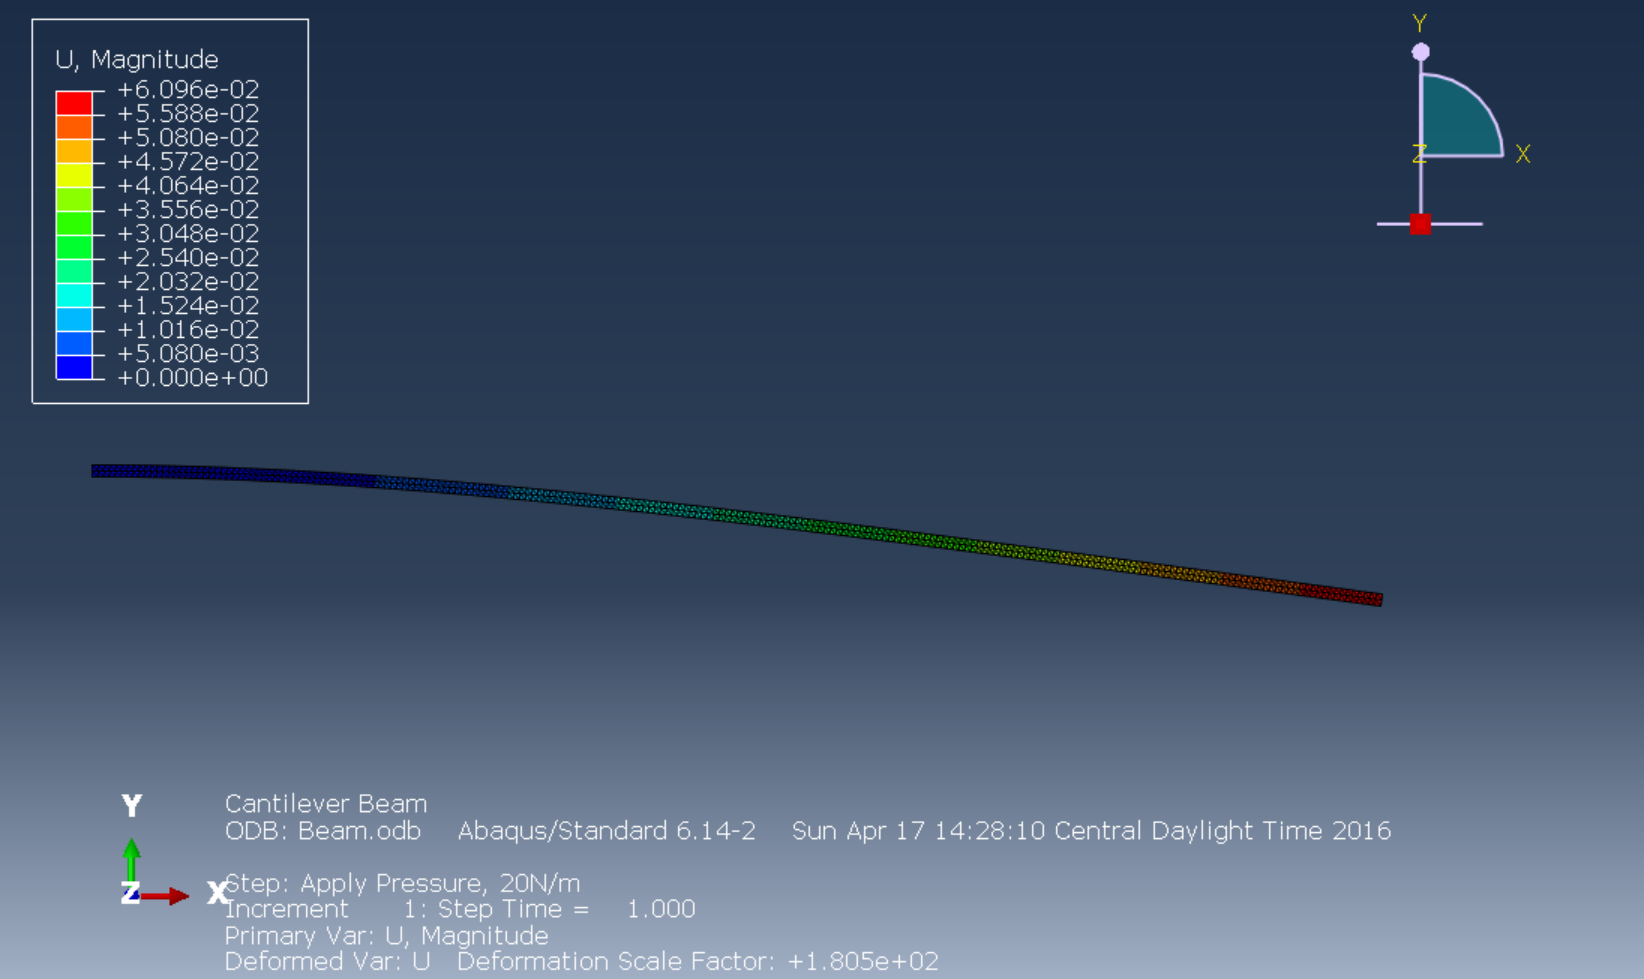
\includegraphics[scale=.5]{6Nsize0_5MDisplacement.PNG}
\caption{Deflection Contour, Element Size: 0.5, Number of Nodes: 2205, Number of Elements: 880, Maximum Deflection: 6.096 cm}
\end{figure}

\begin{figure}[ht]
\centering
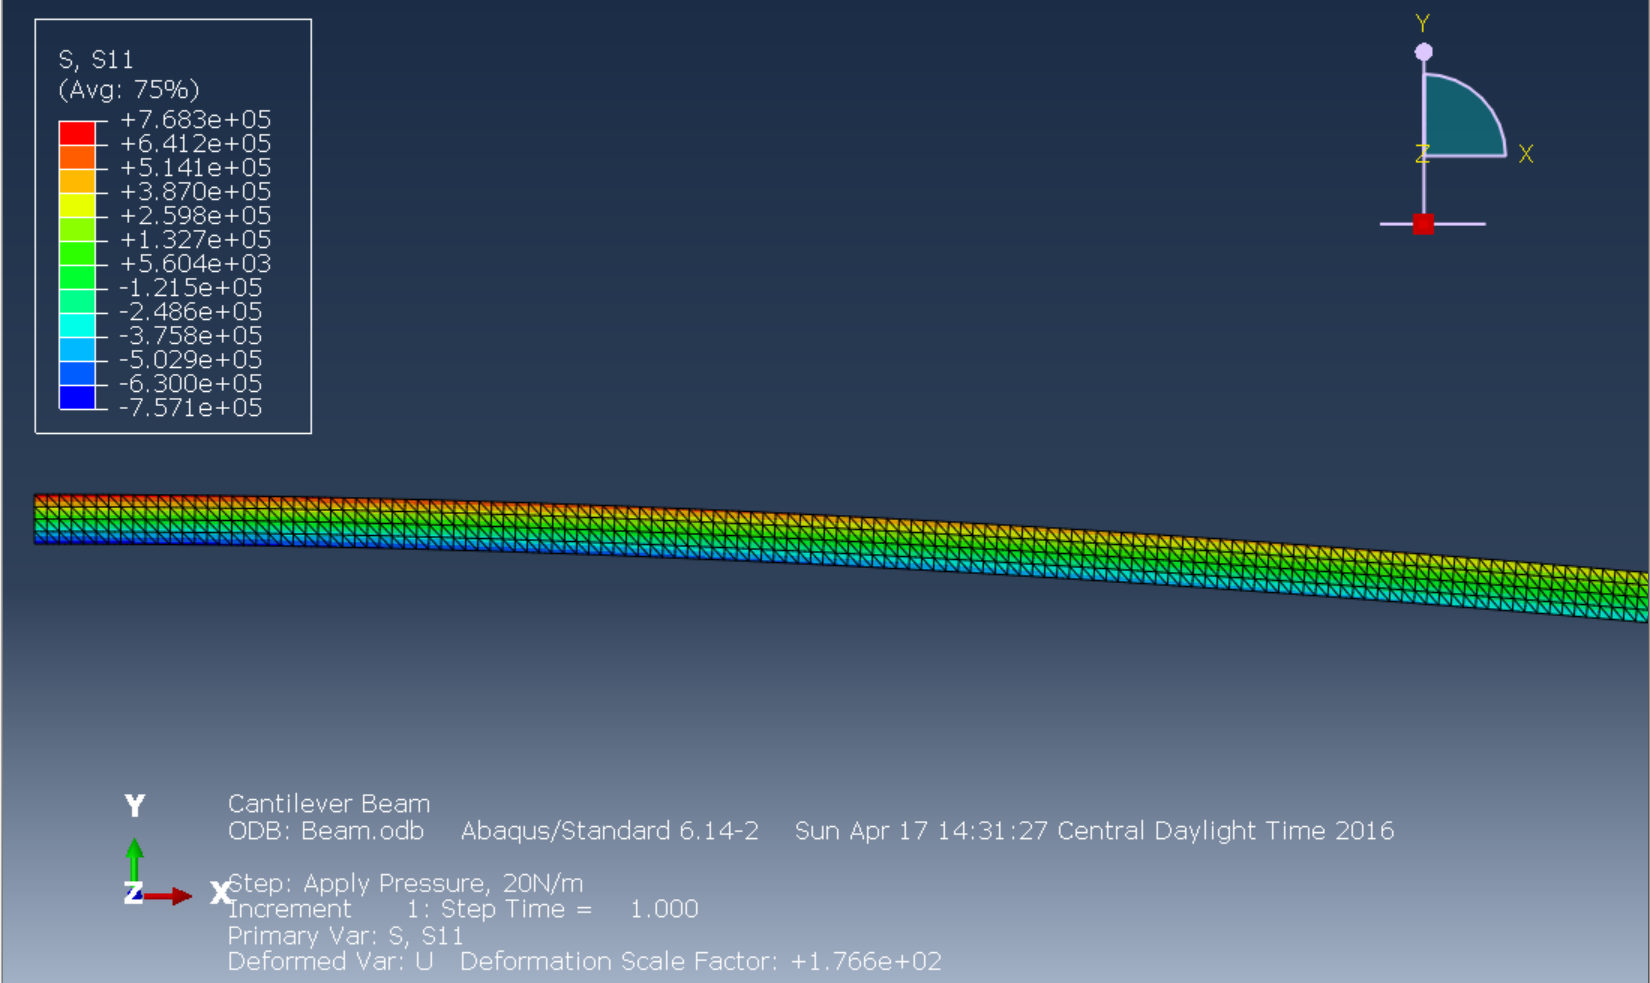
\includegraphics[scale=.5]{6Nsize0_25Stress.PNG}
\caption{Stress Contour, Element Size: 0.25, Number of Nodes: 7929, Number of Elements: 3520}
\end{figure}
\begin{figure}[ht]
\centering
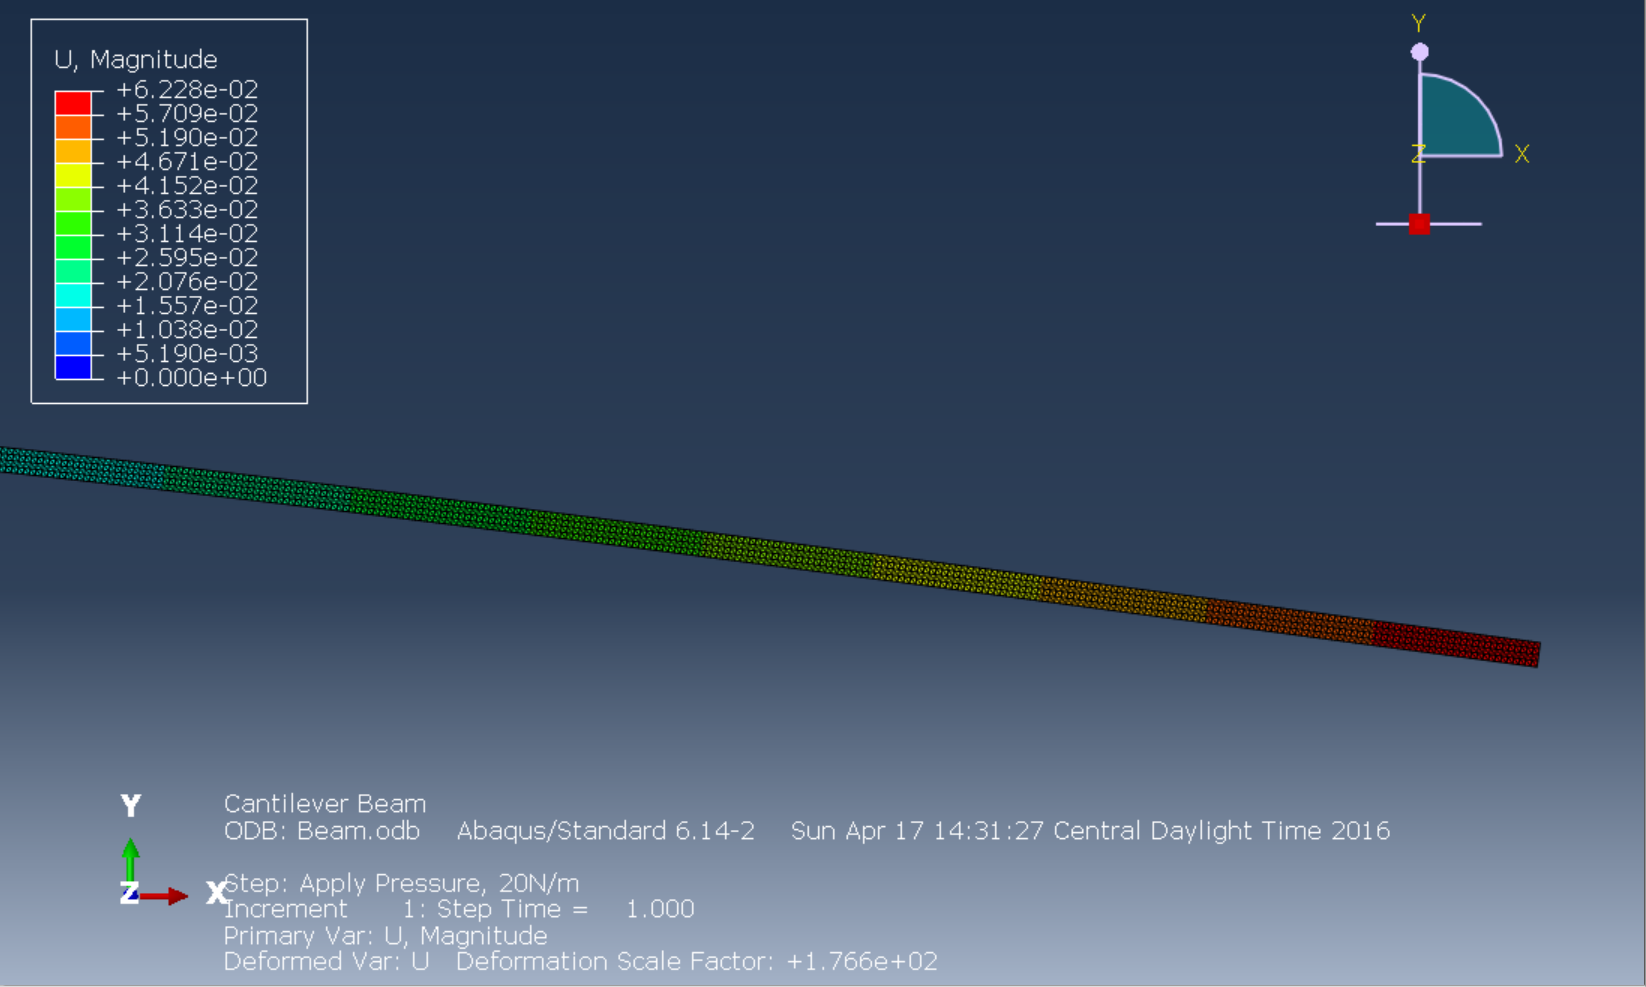
\includegraphics[scale=.5]{6Nsize0_25MDisplacement.PNG}
\caption{Deflection Contour, Element Size: 0.25, Number of Nodes: 7929, Number of Elements: 3520, Maximum Deflection: 6.228 cm}
\end{figure}

\begin{figure}[ht]
\centering
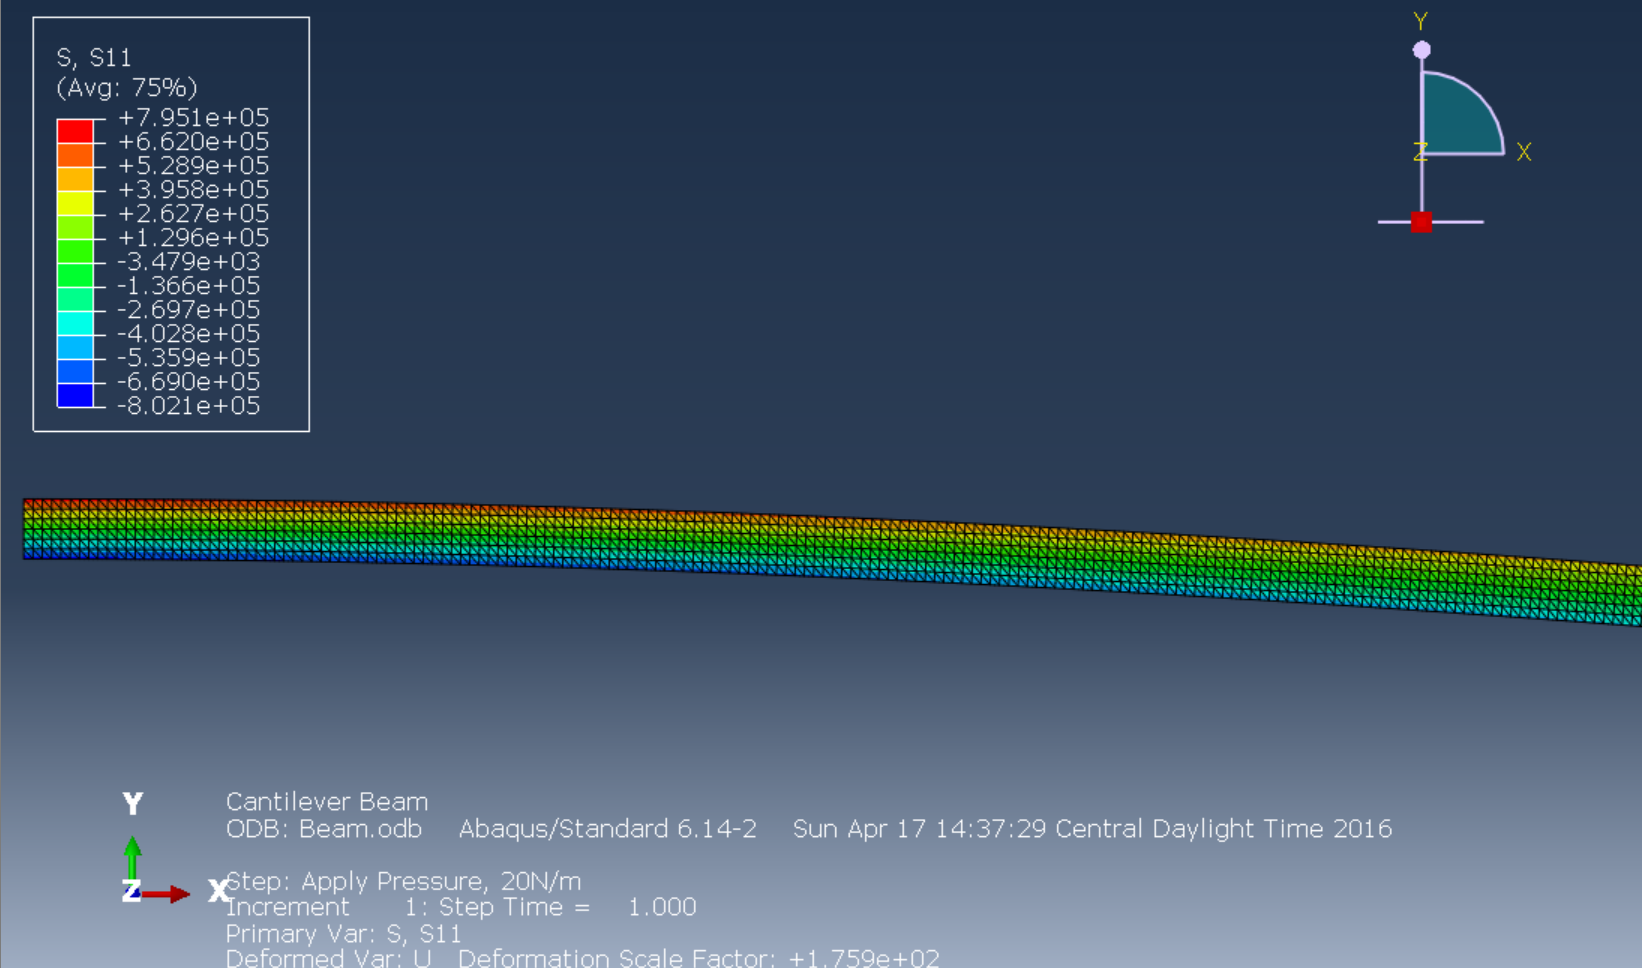
\includegraphics[scale=.5]{6Nsize0_155Stress.PNG}
\caption{Stress Contour, Element Size: 0.155, Number of Nodes: 18,473, Number of Elements: 8520}
\end{figure}
\begin{figure}[ht]
\centering
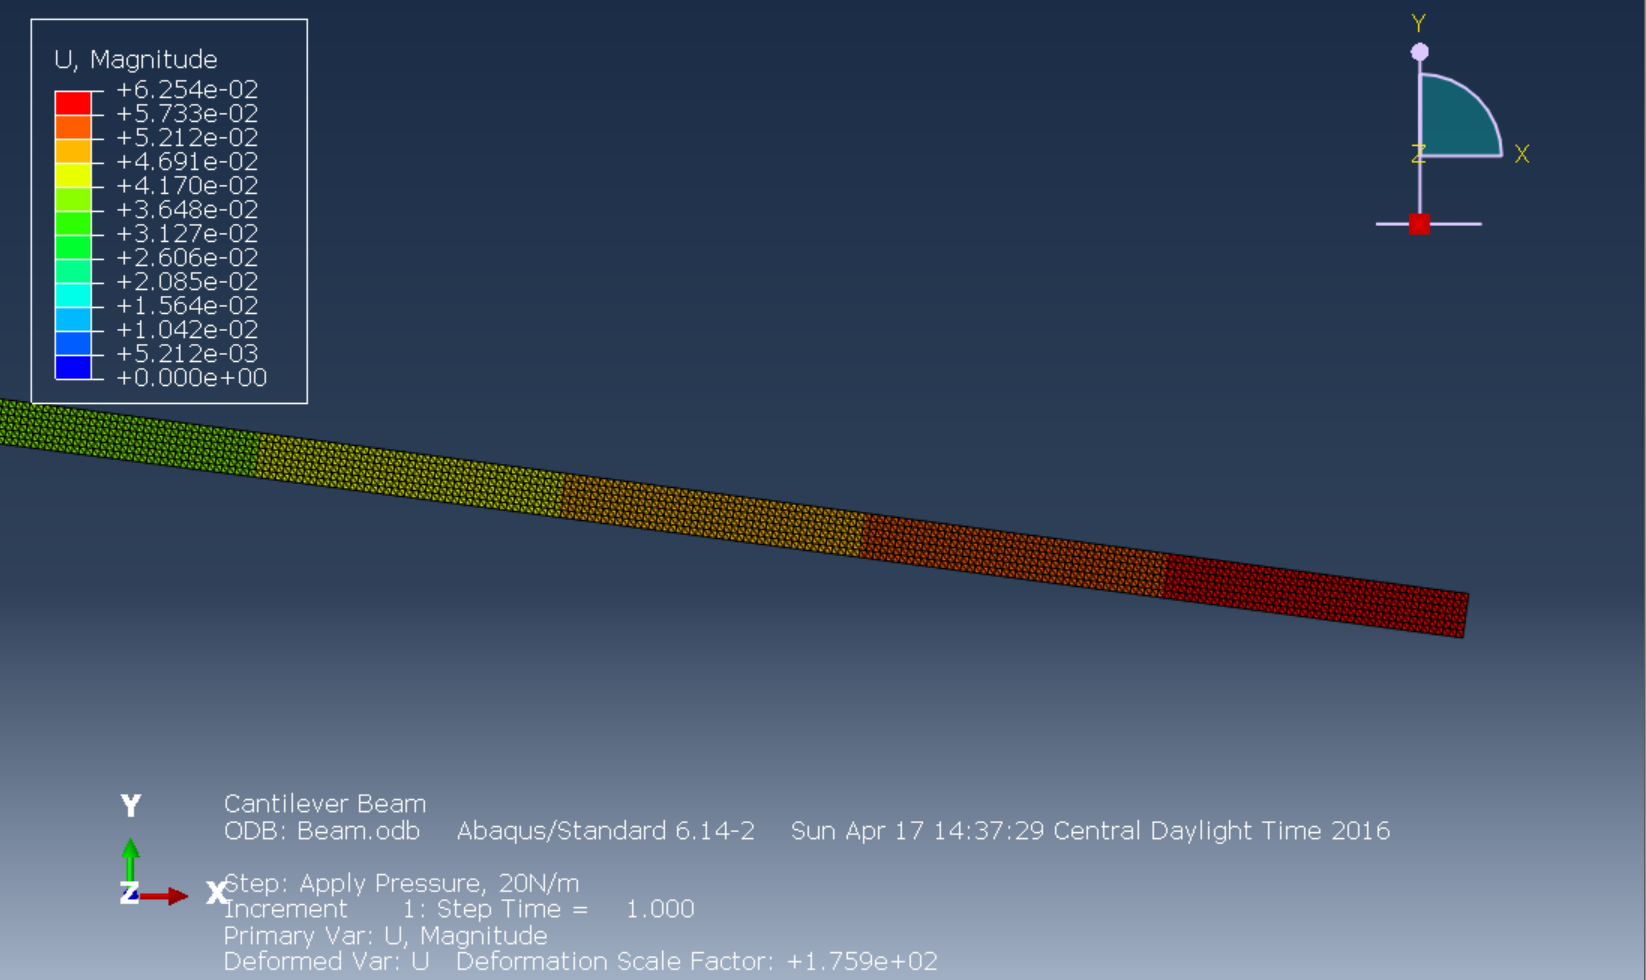
\includegraphics[scale=.5]{6Nsize0_155MDisplacement.PNG}
\caption{Deflection Contour, Element Size: 0.155, Number of Nodes: 18,473, Number of Elements: 8520, Maximum Deflection 6.254 cm}
\end{figure}

\clearpage

\begin{figure}[ht]
\centering
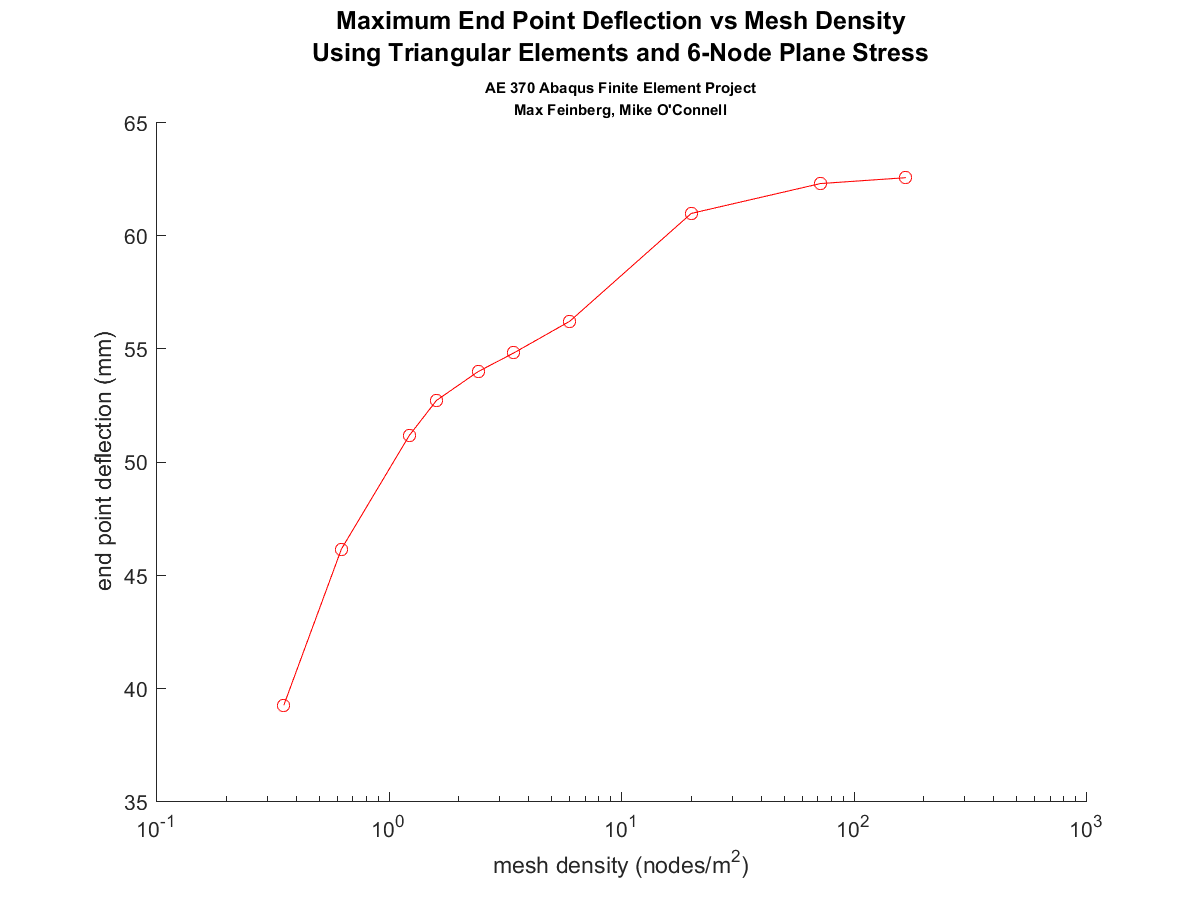
\includegraphics[scale=.65]{ae370abaqus_6node.png}
\caption{A Plot Showing the Convergence of the Maximum Deflection}
\end{figure}

Figure 43 above shows how the maximum deflection of the beam converges as the mesh density of the FEA model increases for the 6-node triangular elements. Similarly to the 3-node triangular element simulations, the 6-node simulations converge to a deflection of roughly 60 mm.  As it can be clearly seen in the plot, the change in end point deflections quickly decreases twice after the mesh density surpasses a value of roughly 1 $\frac{nodes}{m^{2}}$ and again when the mesh density surpasses a value of roughly 100 $\frac{nodes}{m^{2}}$.  Unlike the previous set of simulations, the 6-node simulations experience two periods of quick convergence.\\

To confirm that the solution had indeed converged, the convergence number was calculated as in the previous section.  Using 6-node plane stress triangular elements, a convergence number of .0294 was reached with only 7929 nodes(72.08 $\frac{nodes}{m^{2}}$).  

\clearpage

\textbf{c)}\\

\begin{figure}[ht]
\centering
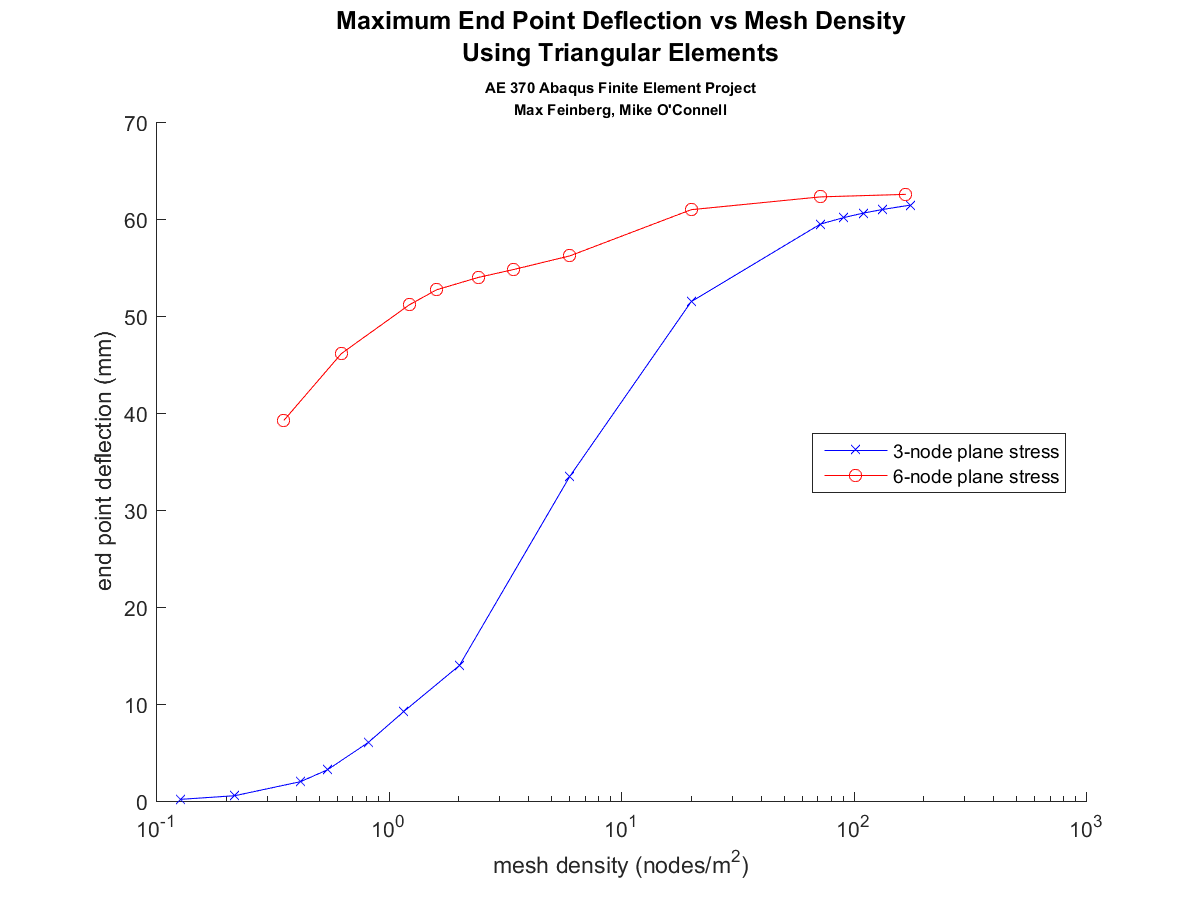
\includegraphics[scale=.65]{ae370abaqus_combined.png}
\caption{A Plot Showing the Convergence of the Maximum Deflection of the Two Sets of Simulations}
\end{figure}

Figure 44 above shows the convergence plots of both the 3-node and 6-node FEA simulations. When the simulations were being conducted, element size was used as the input parameter, using the values of 20, 10, 5, 3.75, 2.5, 1.75, 1, 0.5, 0.25, 0.155, and 0.125. The value of 0.155 was used in the 6-node simulation instead of 0.125 because of the 20,000 node restriction on the University Abaqus license. To more accurately show convergence, the 3-node simulations was also tested with size values of 0.11, 0.1, 0.09, and 0.08.  It can be clearly seen in the graph that the 6-node simulation converges significantly faster than the 3-node simulation.  From our convergence tests, we have also seen that the 6-node simulations achieve a convergence value of 0.0294 with a mesh density of only 72.08 $\frac{nodes}{m^{2}}$ while the 3-node simulations only achieve a convergence value of 0.0437 at a mesh density of 110.1 $\frac{nodes}{m^{2}}$. This indicates that using 6-node elements in FEA simulations generally lead to quicker convergence, and it therefore allows us to use lower mesh densities in our simulations to achieve roughly the same results when compared to simulations that use greater mesh densities of 3-node elements.

\clearpage

\section*{MATLAB Code}

\lstinputlisting[basicstyle=\ttfamily\scriptsize,language=Matlab]{ae370abaqus.m}
\end{document}